\documentclass[12pt,a4paper, oneside]{memoir}
\setsecnumdepth{subsubsection} % pour gérer la profondeur de la numérotation
\settocdepth{subsubsection}  % pour gérer la profondeur de la numérotation dans la table de matière
\usepackage[utf8]{inputenc}
\usepackage[T1]{fontenc}
\usepackage[french]{babel}
\usepackage{amsmath}
\usepackage{graphicx}
\usepackage[colorinlistoftodos]{todonotes}
\usepackage{lmodern} %police
\usepackage[a4paper,margin=1.5cm]{geometry} %marges
\usepackage[most]{tcolorbox}
\usepackage{xcolor} % pour la coloration syntaxique
\usepackage{titlesec}  % Pour styliser les titres si besoin
\usepackage{hyperref}  % Pour les liens cliquables
\usepackage{pgfgantt} % pour le diagramme de Gantt
\usepackage{float}
\usepackage{enumitem}
\usepackage[colorinlistoftodos]{todonotes}
\geometry{margin=2.5cm}
\usepackage[strings]{underscore}

\usepackage{caption}
\usepackage{subcaption}
\usepackage{fancyvrb}
\usepackage{array}
\usepackage{adjustbox}
\usepackage{tabularx} 
\usepackage[table]{xcolor}
\usepackage{multirow}
\usepackage{lscape} %pour un tableau en paysage
\usepackage{pdflscape} %pour un tableau en paysage 


\usepackage{tikz}
%\usepackage{tikz-uml}
\usetikzlibrary{shapes.multipart, arrows.meta, positioning, calc}

\tikzset{
	box/.style={
		draw,
		rounded corners,
		text width=5.5cm,
		minimum height=1.2cm,
		align=center,
		font=\small,
		fill=blue!5
	},
	arrow/.style={
		-{Latex[length=2mm]},
		thick
	}
}

\usetikzlibrary{positioning}
\usetikzlibrary{arrows.meta, shapes.multipart, positioning}
\usepackage{pgf-umlsd}

\usepackage{listings}
\lstdefinelanguage{autoconf}{
	morekeywords={AC_INIT,AC_PREREQ,AC_ARG_ENABLE,AS_HELP_STRING,PKG_CHECK_MODULES,
		AC_CANONICAL_HOST,AC_CANONICAL_TARGET},
	sensitive=true,
	morecomment=[l]\#,
	morestring=[b]"
}

\lstset{
	basicstyle=\ttfamily\small,
	keywordstyle=\color{blue},
	commentstyle=\color{gray},
	stringstyle=\color{red},
	showstringspaces=false,
	breaklines=true,
	frame=single,
	%breaklines=true,          % permet de couper les lignes trop longues
	%	breakatwhitespace=false,  % coupe même au milieu d’un mot si besoin
	%breakatwhitespace=true
	%postbreak=\mbox{\textcolor{red}{$\hookrightarrow$}\space}, % joli symbole de continuation
	%basicstyle=\ttfamily\small,
	%columns=fullflexible
}

%\usepackage[acronym]{glossaries}
%\makeglossaries
\usepackage{tabularx}
\usepackage{booktabs}

%---Entête et pieds de page ---
\usepackage{fancyhdr} % Personnalisation des en-têtes et pieds de page
\usepackage{lastpage}  % Pour connaître la dernère page (pour X/Y)
\pagestyle{fancy} %Active le style fancy
\fancyhf{}       %Vide en-têtes et pieds
\fancyfoot[C]{Page\thepage/\pageref{LastPage}} %Centré en bas : Page 1/2
\renewcommand{\headrulewidth}{0pt}  % Supprime le trait en haut
\renewcommand{\footrulewidth}{0pt}  % Pas de trait en bas (modifiable)

\pagestyle{fancy}
\fancyhf{} % Nettoyer les entêtes et pieds

% --- En-tête gauche : texte ---


% =========================
% En-tête personnalisé GitHub
% =========================

\fancyhead[L]{%
	\begin{minipage}{0.65\textwidth}
		\raggedright
		\textbf{\Large Architecture Réseau d’Entreprise Sécurisée}\\
		\small Urbanisation des Services Réseau -CNAM
	\end{minipage}
}

\fancyhead[R]{%
	% Optionnel : logo
	% \includegraphics[height=1.5cm]{logo.png}
}

\renewcommand{\headrulewidth}{0pt}

\begin{document}
	
	\vspace*{0.85cm}
	
	\begin{center}
		
		{\Huge \textbf{Architecture Réseau d’Entreprise Sécurisée}}\\[0.45cm]
		
		{\Large Conception d’une Infrastructure Multi-Sites}\\[0.9cm]
		
		{\large \textit{MPLS, L2VPN, L3VPN (GRE), OSPF et Sécurisation des Flux}}\\[1cm]
		
		\begin{tcolorbox}[colback=gray!5,colframe=black,width=1\textwidth,sharp corners,boxrule=1pt]
			\centering
			\large
			Ce projet présente la conception et la mise en œuvre d’une architecture réseau d’entreprise complète intégrant :
			
			\vspace{0.3cm}
			
			\begin{itemize}
				\item Une infrastructure multi-sites interconnectée
				\item Une segmentation logique via VLANs
				\item Un plan d’adressage IPv4 structuré et hiérarchisé
				\item Un backbone opérateur IP/MPLS
				\item Des tunnels VPN :
				\begin{itemize}
					\item L2VPN (VPWS) pour l’interconnexion des sites
					\item L3VPN (GRE) pour l’accès au Cloud
				\end{itemize}
				\item Une architecture orientée sécurité (ACL, isolation des flux)
				\item Une validation fonctionnelle (ping, traceroute, Wireshark)
			\end{itemize}
			
		\end{tcolorbox}

		\vspace{1cm}
		
		\textbf{Auteur}\\
		Nozha Safi Jlidat
		
		\vspace{0.5cm}
		
		\textbf{Contexte académique}\\
		Conservatoire National des Arts et Métiers (CNAM)\\
		Urbanisation des Services Réseau
		
		\vspace{0.5cm}
		
		\textbf{Année universitaire}\\
		2025 – 2026
		
		\vspace{1cm}
		
		\rule{\linewidth}{0.4mm}
		
		\vspace{0.5cm}
		
		\small
		Ce dépôt présente une documentation technique reconstruite d’une architecture
		réseau d’entreprise, dans un environnement simulé (GNS3), réalisée dans un cadre pédagogique.
		
	\end{center}
	%--- Fin page de garde ---
	\clearpage
	
	\pagestyle{fancy}
	\fancyhf{}
	
	\tableofcontents
	\newpage
	
	\listoffigures
	\newpage
	
	\listoftables
	\newpage


\chapter{Architecture Réseau de l’Entreprise}

\section{Contexte}

L’entreprise dispose de deux sites géographiquement distincts (\textbf{Site 1} et \textbf{Site 2}). 
Chaque site comprend :

\begin{itemize}
	\item deux réseaux utilisateurs (Administratif et Développeurs),
	\item un réseau de serveurs Intranet,
	\item un réseau de serveurs publics accessibles depuis Internet.
\end{itemize}

En complément, deux sous-réseaux sont hébergés chez un fournisseur \textbf{Cloud} afin :

\begin{itemize}
	\item d’externaliser certains services,
	\item d’absorber les pics de charge,
	\item d’améliorer la résilience globale de l’architecture.
\end{itemize}

Le réseau opérateur (\textit{WAN}) est traité séparément mais reste intégré dans la conception globale de l’architecture réseau.
\subsection{Topologie réseau globale}
La figure suivant en (fig.~\ref{fig:topologie_globale}) présente la topologie globale de l’infrastructure réseau de l’entreprise. 
Cette topologie met en évidence l’organisation physique du réseau
(routeurs, commutateurs et hôtes) ainsi que la segmentation logique
des différents services au moyen de VLAN. Cette approche permet de
séparer les flux utilisateurs, les services Intranet et les services
publics exposés sur Internet, tout en conservant une architecture
cohérente entre les deux sites et l’extension Cloud.

\begin{figure}[H]
	\centering
	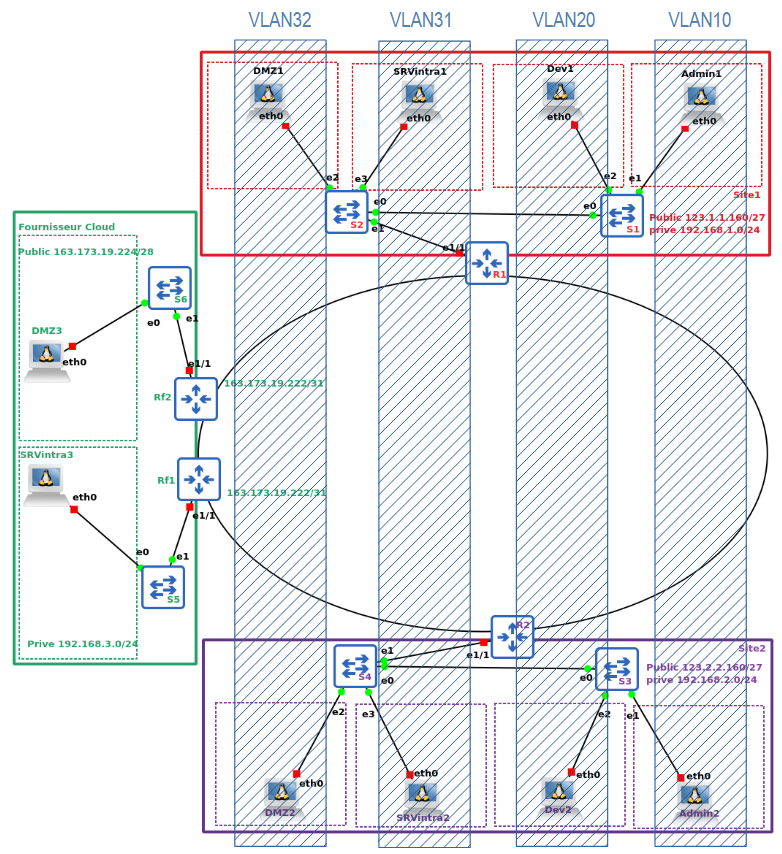
\includegraphics[width=\textwidth]{../captures/01_topologie_globale.png}
	\caption{Topologie globale de l’architecture réseau de l’entreprise incluant les deux sites,
		l’infrastructure Cloud et la segmentation logique des réseaux par VLAN}
	
	\label{fig:topologie_globale}
\end{figure}

Les différentes zones de l’architecture sont représentées par des
codes couleurs permettant d’identifier rapidement les périmètres
réseau : les sites internes de l’entreprise, les segments publics
exposés à Internet ainsi que l’extension de l’infrastructure
hébergée chez le fournisseur Cloud.


\subsection{Convention de nommage}

Les sous-réseaux suivent la notation suivante :

\[
\texttt{LAN\_x-y}
\]

où :

\begin{itemize}
	\item \textbf{x} représente le numéro du site :
	\begin{itemize}
		\item 1 : Site 1
		\item 2 : Site 2
		\item 3 : Infrastructure Cloud
	\end{itemize}
	
	\item \textbf{y} représente l'identifiant fonctionnel du sous-réseau.
\end{itemize}

Cette convention permet d’identifier rapidement l’origine et la fonction de chaque réseau dans l’architecture globale.

\subsection{Structure des LAN et VLAN}
	\begin{enumerate}
		\item \textbf{Organisation des LAN}

\begin{table}[H]
	\centering
	\renewcommand{\arraystretch}{1.3}
	\begin{tabular}{|l|l|}
		\hline
		\textbf{Fonction} & \textbf{Désignation} \\
		\hline
		Administratif & LAN\_1-1 / LAN\_2-1 \\
		Développeurs & LAN\_1-2 / LAN\_2-2 \\
		Serveurs Intranet & LAN\_1-31 / LAN\_2-31 \\
		Serveurs Publics & LAN\_1-32 / LAN\_2-32 \\
		Cloud Intranet & LAN\_3-31 \\
		Cloud Public & LAN\_3-32 \\
		\hline
	\end{tabular}
	\caption{Organisation des sous-réseaux LAN}
\end{table}

	\item \textbf{Segmentation VLAN}

\begin{table}[H]
	\centering
	\renewcommand{\arraystretch}{1.3}
	\begin{tabular}{|l|l|}
		\hline
		\textbf{VLAN} & \textbf{Usage} \\
		\hline
		VLAN\_10 & Département Administratif \\
		VLAN\_20 & Département Développeurs \\
		VLAN\_31 & Serveurs Intranet (privés) \\
		VLAN\_32 & Serveurs publics accessibles depuis Internet \\
		\hline
	\end{tabular}
	\caption{Segmentation VLAN}
\end{table}
\end{enumerate}

Cette segmentation permet :

\begin{itemize}
	\item une isolation logique des flux réseau,
	\item un contrôle précis des communications via des ACL,
	\item une amélioration de la sécurité globale du système,
	\item une meilleure évolutivité de l’infrastructure.
\end{itemize}

\subsection{Principes d’architecture}
Cette architecture a été conçue selon des principes d’ingénierie réseau visant à garantir robustesse, sécurité et évolutivité de l’infrastructure. Elle repose sur les principes suivants :

\begin{itemize}
	\item une séparation stricte des rôles entre utilisateurs, serveurs internes et services publics ;
	\item une distinction claire entre l’adressage privé interne et l’adressage public exposé à Internet ;
	\item une hiérarchisation du réseau facilitant l’application des politiques de sécurité ;
	\item une capacité d’évolution du réseau sans remise en cause du plan d’adressage initial.
\end{itemize}

\subsection{Recensement des sous-réseaux}

Chaque sous-réseau est défini selon les critères suivants :

\begin{itemize}
	\item le nom du sous-réseau,
	\item le type d’adressage (privé ou public),
	\item le nombre d’hôtes requis,
	\item le rôle fonctionnel dans l’architecture.
\end{itemize}

\begin{enumerate}
	\item \textbf{Site 1}

\begin{table}[H]
	\centering
	\renewcommand{\arraystretch}{1.3}
	\begin{tabular}{|l|l|c|l|}
		\hline
		\textbf{Sous-réseau} & \textbf{Adressage} & \textbf{Hôtes} & \textbf{Rôle} \\
		\hline
		LAN\_1-1 & Privé & 14 & Département Administratif \\
		LAN\_1-2 & Privé & 18 & Département Développeurs \\
		LAN\_1-31 & Privé & 6 & Serveurs Intranet locaux \\
		LAN\_1-32 & Public & 14 & Serveurs exposés à Internet \\
		\hline
	\end{tabular}
	\caption{Sous-réseaux du Site 1}
\end{table}

	\item \textbf{Site 2}

\begin{table}[H]
	\centering
	\renewcommand{\arraystretch}{1.3}
	\begin{tabular}{|l|l|c|l|}
		\hline
		\textbf{Sous-réseau} & \textbf{Adressage} & \textbf{Hôtes} & \textbf{Rôle} \\
		\hline
		LAN\_2-1 & Privé & 7 & Département Administratif \\
		LAN\_2-2 & Privé & 26 & Département Développeurs \\
		LAN\_2-31 & Privé & 2 & Serveurs Intranet locaux \\
		LAN\_2-32 & Public & 6 & Serveurs exposés à Internet \\
		\hline
	\end{tabular}
	\caption{Sous-réseaux du Site 2}
\end{table}

	\item \textbf{Infrastructure Cloud}

\begin{table}[H]
	\centering
	\renewcommand{\arraystretch}{1.3}
	\begin{tabular}{|l|l|c|l|}
		\hline
		\textbf{Sous-réseau} & \textbf{Adressage} & \textbf{Hôtes} & \textbf{Rôle} \\
		\hline
		LAN\_3-31 & Privé & 10 & Serveurs Intranet externalisés \\
		LAN\_3-32 & Public & 10 & Serveurs publics hébergés dans le Cloud \\
		\hline
	\end{tabular}
	\caption{Sous-réseaux Cloud}
\end{table}
\end{enumerate}
\subsection{Paramètres définis pour chaque sous-réseau}

Pour chaque sous-réseau, les éléments suivants sont formellement définis :

\begin{itemize}
	\item l’adresse réseau (\textit{Network Address}),
	\item le masque CIDR,
	\item l’adresse de diffusion (\textit{Broadcast Address}),
	\item la première adresse IP utilisable attribuée à la passerelle (\textit{Gateway}).
\end{itemize}

Cette normalisation garantit :

\begin{itemize}
	\item une cohérence d’implémentation du plan d’adressage,
	\item une meilleure lisibilité de la configuration réseau,
	\item une maintenance facilitée,
	\item une compatibilité avec les mécanismes de sécurité tels que les politiques \textbf{NAT} et les \textbf{ACL}.
\end{itemize}

%%%%%%%%%%%%%%%%%%%%%%%%%%%%%%%%%%%%%%%%%%%%%%%%%%%%

\section{Plan d’adressage IP}
Les détails complets du calcul des sous-réseaux et des plages d’adresses sont présentés dans la feuille de calcul associée.

\subsection{Stratégie Globale d’Adressage Privé}
Le plan d’adressage interne s’appuie sur le bloc IP privé \texttt{192.168.0.0/16}. 
Chaque site utilise un sous-réseau dédié en /24.\\
\begin{enumerate}
	\item Site 1 → 192.168.1.0/24	
	\item Site 2 → 192.168.2.0/24	
	\item Cloud → 192.168.3.0/24
\end{enumerate}


Les sous-réseaux sont dimensionnés en fonction des besoins réels en hôtes, tout en conservant une marge d’évolution et une cohérence d’ensemble.

\subsection{Plan d'adressage - Site 1}

\begin{enumerate}
	\item \textbf{Plage d’adressage privé}

\begin{table}[]
	\centering
	\begin{tabular}{|c|l|c|c|c|c|}
		\hline
		\textbf{LAN} &  \textbf{Réseau/Masque}  & \textbf{IP réseau} & \textbf{BroadCast} & \textbf{Plage IP hôtes} & \textbf{Passerelle} \\
		\hline
		LAN\_1-1   & 192.168.1.0/27 &  192.168.1.0 & 192.168.1.31 & 192.168.1. 1$\leftrightarrow$ .1.30 & 192.168.1.1 \\
		LAN\_1-2   & 192.168.1.32/27 & 192.168.1.32 & 192.168.1.63  & 192.168.1.33 $\leftrightarrow$ .1.62 & 192.168.1.33\\
		LAN\_1-31 & 192.168.1.64/29 &192.168.1.64 & 192.168.1.71 & 192.168.1.65 $\leftrightarrow$ .1.70 & 192.168.1.65 \\
		\hline
	\end{tabular}
	\caption{Sous-réseaux privés du Site 1}
\end{table}
	\vspace{0.5cm}
	
	\begin{enumerate}
		\item Les LAN utilisateurs sont en /27 afin d’assurer une capacité d’évolution et une homogénéité d’architecture.\\
		\item Le LAN serveurs Intranet utilise un /29, suffisant pour 6 hôtes.\\
		\item La première adresse IP utilisable est attribuée à la passerelle par défaut.	\\ 
	\end{enumerate}
 
	\item \textbf{Gestion de la plage publique}

Le Site 1 dispose du bloc public suivant : \texttt{123.1.1.160/27} (30 adresses IP utilisables).\\
Ce bloc est subdivisé afin de couvrir plusieurs besoins : 
\begin{itemize}[label*=$\rightarrow$]
	\item Hébergement des serveurs publics (LAN\_1-32)
	\item Liaison WAN opérateur
	\item Pool NAT pour les postes internes
\end{itemize}
%------------------------------------------

\begin{table}[H]
	\centering
	\renewcommand{\arraystretch}{1.3}
	\begin{tabular}{|l|l|}
		\hline
		\rowcolor{gray!10}
		\textbf{\textit{LAN\_1-32 (Serveurs publics)}} & \textbf{\textit{Adressage IPv4}}\\
		\hline
		\textbf{Plage d'adressage} & \textbf{\textit{123.1.1.160/28}} \\
		\hline
		Réseau & 123.1.1.160 \\
		\hline
		Adresse de broadcast & 123.1.1.175 \\
		\hline
		Plage d'adresses utilisables & 123.1.1.161 -- 123.1.1.174 \\
		\hline
		Passerelle  & 123.1.1.161 (ou .162)\\
		\hline
		Nombre d'adresses utilisables & 14 \\
		\hline	
		\hline
		\textbf{\textit{Liaison WAN point-à-point opérateur}} & \textbf{\textit{123.1.176/31}}\\
		\hline
		R1 $\leftrightarrow$ Op & 123.1.1.176 $\leftrightarrow$ 123.1.1.177\\
		\hline
		\hline
		\textbf{\textit{Pool NAT dynamique}} (postes internes) & \textbf{\textit{123.1.1.178 à 123.1.1.190}} \\
		\hline
		Nombre d'adresses IP NAT & 13\\
		\hline
	\end{tabular}
	\caption{Découpage de la plage publique du Site 1}
\end{table}

L’ensemble de ces sous-réseaux reste inclus dans la plage publique initiale 
\textbf{123.1.1.160/27}. Cette approche permet :

\begin{itemize}
	\item d’allouer des adresses publiques fixes aux serveurs exposés (NAT statique),
	\item de réserver un bloc pour la liaison WAN,
	\item d’implémenter un NAT dynamique pour les VLAN internes,
	\item tout en optimisant l’utilisation de l’espace d’adressage public tout en garantissant évolutivité et séparation des fonctions..
\end{itemize}

\vspace{0.5cm}
\item \textbf{Polique NAT }

\textit{NAT Statique (1:1)} : Les serveurs exposés utilisent un NAT statique (1:1) \textit{1 adresse IP privée $\leftrightarrow$ 1 adresse publique}.

\textit{Objectifs }:
\begin{itemize}[label*=$\star$]
	\item Adresse publique permanente
	\item Publication DNS possible
	\item Accessibilité continue depuis Internet
\end{itemize} 


\textit{NAT Dynamique avec surcharge (PAT)} : Les Vlan internes utilisent un pool d'adresses publiques, \textit{Nat avec surcharge (PAT)} et une traduction basée sur les ports. 

Cela permet à plusieurs machines privées de partager une ou plusieurs adresses publiques.
\end{enumerate}
%---------------------

\subsection{Plan d'adressage - Site 2}

\begin{enumerate}
	\item \textbf{Gestion de la plage privée}

\begin{table}[H]
	\centering
	\begin{tabular}{|c|l|c|c|c|c|}
		\hline
		\textbf{LAN} &  \textbf{Réseau/Masque}  & \textbf{IP réseau} & \textbf{BroadCast} & \textbf{Plage IP hôtes} & \textbf{Passerelle} \\
		\hline
		LAN\_2-1   & 192.168.2.0/27 &  192.168.2.0 & 192.168.2.31 & 192.168.2.1 $\leftrightarrow$ .2.30 & 192.168.2.1 \\
		LAN\_2-2   & 192.168.2.32/27 & 192.168.2.32 & 192.168.2.63 & 192.168.2.33 $\leftrightarrow$ .2.62 & 192.168.2.33 \\
		LAN\_2-31 & 192.168.2.64/29 &192.168.2.64 & 192.168.2.71 & 192.168.2.65 $\leftrightarrow$ .2.70& 192.168.2.65 \\
		\hline
	\end{tabular}
	\caption{Sous-réseaux privés du Site 2}
\end{table}
%\vspace{0.5cm}

L’uniformité des masques garantit une cohérence d’architecture entre les deux sites.

\vspace{0.5cm}

\item \textbf{Gestion de la plage publique}

Le Site 2 dispose du bloc public suivant : \texttt{123.2.2.160/27}

\begin{table}[H]
	\centering
	\renewcommand{\arraystretch}{1.3}
	\begin{tabular}{|l|l|}
		\hline
		\rowcolor{gray!10}
		\textbf{\textit{LAN\_2.32 (Serveurs publics)}} & \textbf{\textit{Adressage IPv4}} \\
		\hline
		\textbf{Plan d'adressage} & \textbf{\textit{123.2.2.160/29}} \\
		\hline
		Réseau & 123.2.2.160 \\
		\hline
		BroadCast & 123.2.2.167\\
		\hline
		Plage d'adresses utilisables & 123.2.2.161 -- 123.2.2.166 \\
		\hline
		Passerelle & 123.2.2.161 (ou .162)\\
		\hline
		Nombre d'adresses utilisables & 6 \\
		\hline
		\hline
		\textbf{\textit{Liaison WAN point-à-point opérateur}} & \textbf{\textit{123.2.2.168/31}}\\
		\hline
		R2 $\leftrightarrow$ Op & 123.2.2.168 $\leftrightarrow$ 123.2.2.169\\
		\hline
		\hline
		\textbf{\textit{Pool NAT dynamique}} (postes internes) & \textbf{\textit{123.2.2.170 à 123.2.2.190}} \\
		\hline
		Nombre d'adresses IP NAT & 21 \\
		\hline
	\end{tabular}
	\caption{Découpage de la plage publique du Site 2}
\end{table}
\end{enumerate}
\subsection{Plan d'adressage - Cloud}
\begin{enumerate}
	\item \textbf{Réseau privé Cloud (Intranet) (LAN\_3-31)}

	Le LAN\_3-31 dispose du bloc public suivant :	\texttt{192.168.3.0/28}

	\begin{itemize}[label*=*]
		\item  Ce sous-réseau privé héberge les \textit{serveurs Intranet externalisés} de l’entreprise au sein de l’infrastructure Cloud.  
		
		\item  Il permet d’augmenter la capacité de traitement des services internes tout en conservant une architecture cohérente avec les réseaux locaux des deux sites.
		
		\item  L’accès à ce réseau se fait via \textit{un routage inter-sites} assuré par le routeur \textbf{RF1}, permettant aux différents sites de l’entreprise d’accéder aux services Intranet hébergés dans le Cloud.
		
		\item  Ce réseau \textit{n’est pas exposé directement à Internet}. Les communications sont limitées aux flux internes autorisés, via des mécanismes de filtrage et de routage inter-sites.
	\end{itemize}
	

	%---------------------
	
	\item \textbf{Réseau publique Cloud (Internet) (Lan\_3-32)}
	
	Le sous-réseau LAN\_3-32 correspond à la zone publique hébergée chez le fournisseur Cloud.
	Il est destiné à accueillir des serveurs applicatifs accessibles depuis Internet. Contrairement aux réseaux internes de l’entreprise, ce sous-réseau utilise un adressage IP public (routable via le routeur Rf2), permettant l’accessibilité directe depuis l’extérieur.

	\vspace{0.5cm}

	Le fournisseur Cloud met à disposition la plage publique suivante : \texttt{163.173.19.224/28}

\begin{table}[H]
	\centering
	\renewcommand{\arraystretch}{1.3}
	\begin{tabular}{|l|l|}
		\hline
		\rowcolor{gray!20}
		 \textbf{\textit{LAN\_3-32 (Serveurs publics Cloud)}} & \textbf{\textit{Adressage IPv4}} \\
		\hline
		\textbf{Plage d'adressage} & \textbf{163.173.19.224/28} \\
		\hline
		Réseau & 163.173.19.224 \\
		\hline
		Plage d'adresses utilisables & 163.173.19.225 -- 163.173.19.238 \\
		\hline
		Nombre d'adresses utilisables & 14 \\
		\hline
		Passerelle (Routeur Rf2) & 163.173.19.225 \\
		\hline
		Adresse de broadcast & 163.173.19.239 \\
		\hline
		\hline
		\textbf{Liaison WAN point-à-point opérateur} & \textbf{163.173.19.222/31}\\
		\hline
		Rf2 $\leftrightarrow$ op &	163.173.19.222 $\leftrightarrow$ 163.173.19.223\\
		\hline
	\end{tabular}
	\caption{Paramètres du sous-réseau public Cloud LAN\_3-32}
\end{table}


	Le routeur Rf2 assure l’interconnexion entre le réseau public Cloud (LAN\_3-32) et le réseau de l’opérateur via une liaison point-à-point utilisant le sous-réseau 163.173.19.222/31.
\end{enumerate}
%----------------------

\subsection{Configuration des interfaces réseau des hôtes}

Afin de vérifier la connectivité de la topologie réseau mise en place dans l’environnement GNS3, les interfaces réseau des différentes machines ont été configurées manuellement avec des adresses IP statiques.

Dans un premier temps, cette configuration statique permet de valider le bon fonctionnement du plan d’adressage et des routes avant la mise en place de services automatisés tels que DHCP.

\begin{enumerate}
	\item \textbf{Méthodes de configuration}

Sous les systèmes Linux utilisés dans la topologie, la configuration des interfaces réseau peut être réalisée de deux manières :

\begin{itemize}
	\item en mode texte, en modifiant directement le fichier de configuration situé dans :
	\texttt{/etc/network/interfaces}
	\item en mode graphique, en effectuant un clic droit sur la machine concernée dans GNS3 puis en sélectionnant l’option \textit{Edit Configuration}.
\end{itemize}

Avant tout, il faut redémarrer le service réseau : 

\texttt{/etc/init.d/networking start ou restart}, 

ou bien redémarrer la machine.

Dans le cas de la configuration manuelle, il est nécessaire d’activer les lignes correspondantes à l’interface réseau en supprimant les caractères de commentaire (\#), puis de renseigner les paramètres réseau appropriés.

\item \textbf{Paramètres configurés}

Les paramètres suivants doivent être définis pour chaque interface :

\begin{itemize}
	\item l’adresse IP de l’interface ;
	\item le masque de sous-réseau (\textit{netmask}) ;
	\item l’adresse de la passerelle par défaut (\textit{gateway}).
\end{itemize}

\item \textbf{Exemple de configuration}

Un exemple de configuration statique d’une interface réseau dans le fichier
\texttt{/etc/network/interfaces} est présenté ci-dessous :

\begin{verbatim}
	auto eth0
	iface eth0 inet static
	address 192.168.1.34
	netmask 255.255.255.224
	gateway 192.168.1.33
\end{verbatim}


\begin{figure}[H]
\centering
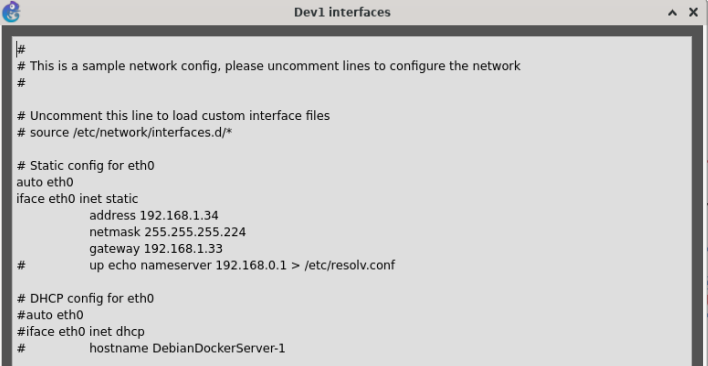
\includegraphics[width=\textwidth]{../captures/02_hote_config_stat.png}
\caption{Exemple de fichier de configuration IP d’une interface réseau en mode graphique}

\label{fig:config_stat}
\end{figure}

Après modification du fichier de configuration, il est nécessaire de redémarrer le service réseau afin d’appliquer les changements :

\begin{verbatim}
	/etc/init.d/networking restart
\end{verbatim}

ou bien de redémarrer la machine.

\item \textbf{Organisation de l'adressage}

Chaque sous-réseau est configuré avec un masque adapté aux besoins en nombre d’hôtes, conformément au plan d’adressage défini précédemment.

Les premières adresses IP utilisables de chaque sous-réseau sont attribuées aux interfaces des routeurs, qui jouent le rôle de passerelles par défaut pour les machines du réseau.

Cette organisation permet d’assurer :

\begin{itemize}
	\item une gestion cohérente de l’espace d’adressage IP ;
	\item une connectivité fiable entre les différents sous-réseaux ;
	\item une communication correcte entre les réseaux internes, le Cloud et l’accès Internet.
\end{itemize}
\end{enumerate}
\subsection{Politique d'adressage}
Pour chaque sous-réseau :
\begin{itemize}[label*=$\star$]
	\item La première adresse IP utilisable est attribuée à l’interface routeur.
	\item Les adresses réseau et broadcast sont exclues.
	\item Les masques sont dimensionnés selon les besoins réels avec marge contrôlée.
	\item Les plages d’adresses sont organisées de manière hiérarchique afin de faciliter l’agrégation des routes et la lisibilité du plan d’adressage.
	
\end{itemize}

%----------------------

\subsection{Considérations de sécurité}

L’exposition de certains services sur Internet impose la mise en œuvre
de mesures de sécurité adaptées afin de protéger l’infrastructure
interne de l’entreprise et de contrôler les flux réseau.

Les principaux mécanismes de sécurité mis en place dans cette architecture sont les suivants :

\begin{itemize}
	\item Filtrage des flux réseau à l’aide d’ACL configurées sur les routeurs d’accès et les équipements de bordure (R1, R2 et Rf2).
	\item Limitation des ports accessibles depuis Internet afin de réduire la surface d’attaque.
	\item Séparation stricte entre les réseaux internes (VLAN utilisateurs et intranet) et les réseaux publics exposés.
	\item Journalisation des connexions afin de permettre une traçabilité des accès et une analyse en cas d’incident de sécurité.
\end{itemize}

Cette approche permet de maintenir une isolation claire entre
l’infrastructure interne de l’entreprise et les services exposés au public,
tout en bénéficiant de la flexibilité offerte par l’extension de
l’infrastructure vers le Cloud.

\subsection{Principes d’architecture appliqués}

La conception du plan d’adressage et de l’architecture réseau repose sur plusieurs principes visant à garantir cohérence, évolutivité et sécurité :

\begin{itemize}
	\item \textbf{Optimisation CIDR} : utilisation de masques de sous-réseau adaptés aux besoins réels en nombre d’hôtes afin d’optimiser l’espace d’adressage.
	
	\item \textbf{Segmentation logique par VLAN} : séparation des différents départements et zones serveurs afin de limiter les communications inutiles et d'améliorer la sécurité.
	
	\item \textbf{NAT statique pour les services exposés} : les serveurs accessibles depuis Internet disposent d’adresses publiques dédiées, permettant leur publication tout en conservant une architecture interne structurée.
	
	\item \textbf{NAT dynamique avec surcharge (PAT)} : les postes utilisateurs des réseaux internes accèdent à Internet via une traduction d’adresse dynamique, permettant le partage d’un nombre limité d’adresses publiques.
	
	\item \textbf{Uniformité multi-sites} : les deux sites de l’entreprise utilisent une architecture réseau similaire, facilitant l’administration, le dépannage et l’évolutivité de l’infrastructure.
	
	\item \textbf{Utilisation efficace de l’espace d’adressage public} : la plage publique attribuée à chaque site est découpée afin d’accueillir les serveurs exposés, les liaisons WAN et les pools NAT, tout en évitant le gaspillage d’adresses IP.
\end{itemize}


%%%%%%%%%%%%%%%%%%%%%%%%%%%%%%%%%%%%%%%%%%%%%%%%%%%%%%%%%%%%%%%%%%%%%


\section{Segmentation réseau et mise en œuvre des VLAN}

\subsection{Principe de segmentation par VLAN}
Pour isoler le trafic des 4 sous-réseaux privés dans chaque site, on va mettre en place des réseaux virtuels (VLAN) de type 802.1q, qu'on les nommera comme ci-dessous : Administratif (VLAN_10), Développeurs (VLAN_20) et Serveurs (VLAN_31 et VLAN_32).

Dans cette configuration, aucune opération particulière n’est requise sur les hôtes, puisque l’appartenance aux VLANs est entièrement gérée au niveau des commutateurs d’accès. Chaque port de ces commutateurs est configuré pour appartenir à un VLAN spécifique. À chaque VLAN est associé un identifiant (ID) unique, ainsi qu’un sous-réseau privé correspondant. Tous les VLANs sont implémentés conformément à la norme IEEE 802.1Q, permettant ainsi la création de réseaux virtuels isolés au sein de l’infrastructure physique.
%---------------------

\subsection{Plan de répartition des VLAN dans l’architecture}
La répartition des VLAN suit la topologie vu sur la figure  \ref{fig:topologie_globale}
\begin{table}[H]
	\centering
	\caption{Affectation des VLANs, interfaces et sous-réseaux par site}
	\label{tab:vlans}
	\renewcommand{\arraystretch}{1.2}
	\begin{tabular}{|c|c|c|c|c|c|c|}
		\hline
		\textbf{VLAN} & \textbf{Département} & \textbf{Site} & \textbf{Switch} & \textbf{Interface} & \textbf{ID VLAN} & \textbf{Réseau} \\
		\hline
		VLAN\_10 & Admin    & 1 & S1 & e1 & 10 & 192.168.1.0/27 \\
		VLAN\_10 & Admin    & 2 & S3 & e1 & 10 & 192.168.2.0/27 \\
		\hline
		\hline
		VLAN\_20 & Dév     & 1 & S1 & e2 & 20 & 192.168.1.32/27 \\
		VLAN\_20 & Dév     & 2 & S3 & e2 & 20 & 192.168.2.32/27 \\
		\hline
		\hline
		VLAN\_31 & SRVintra     & 1 & S2 & e2 & 31 & 192.168.1.64/29 \\
		VLAN\_31 & SRVintra     & 2 & S4 & e2 & 31 & 192.168.2.64/29 \\
		\hline
		\hline
		VLAN\_32 & SRVinter     & 1 & S2 & e3 & 32 & 123.1.1.160/28 \\
		VLAN\_32 & SRVinter     & 2 & S4 & e3 & 32 & 123.2.2.160/29 \\
		\hline
	\end{tabular}
\end{table}
%----------------------

\subsection{Configuration des VLAN sur les commutateurs}

	\begin{enumerate}
		\item \textbf{Architecture des ports des commutateurs}
%Pour chaque site, les VLAN seront configurés sur les switches, et chaque port de switch sera assigné à un VLAN spécifique selon les utilisateurs ou les serveurs qu'il dessert. Les VLAN seront étiquetés avec le protocole IEEE 802.1q afin de permettre le transport simultané des trames appartenant à plusieurs VLANs entre les switches.

La configuration des interfaces se fera comme suit :
		\begin{itemize}
			\item \textbf{Sur les switches S1 et S3}

\textbf{Interface \texttt{e0}} : configurée en mode trunk (802.1q), ce port permet le transport des trames de plusieurs VLANs entre les switches.

\textbf{Interface \texttt{e1}} : configurée en mode access, ce port connecte les machines hôtes appartenant au VLAN\_10 (ID VLAN 10).

\textbf{Interface \texttt{e2}} : configurée en mode access, ce port connecte les machines hôtes appartenant au VLAN\_20 (ID VLAN 20).

		\item \textbf{Sur les switches S2 et S4}

\textbf{Interface \texttt{e0}} : configurée en mode trunk (802.1q), assurant la connexion entre les différents VLANs.

\textbf{Interface \texttt{e1}} : configurée également en mode trunk (802.1q), permettant le transport des trames multi-VLAN.

\textbf{Interface \texttt{e2}} : configurée en mode access, connectant les machines hôtes appartenant au VLAN\_31 (ID VLAN 31).

\textbf{Interface \texttt{e3}} : configurée en mode access, connectant les machines hôtes appartenant au VLAN\_32 (ID VLAN 32).
	\end{itemize}

	\item \textbf{Configuration des VLAN sur le switch S1}

		\begin{itemize}
			\item \textbf{Configuration en mode graphique \\}
		Voici les étapes de configuration des VLANs 10 et 20 sur le commutateur \textbf{S1}, ainsi que l’affectation des interfaces aux VLANs et la configuration du mode \texttt{trunk} pour l’interface connectée au routeur R1.
		\begin{figure}[H]
			\centering
			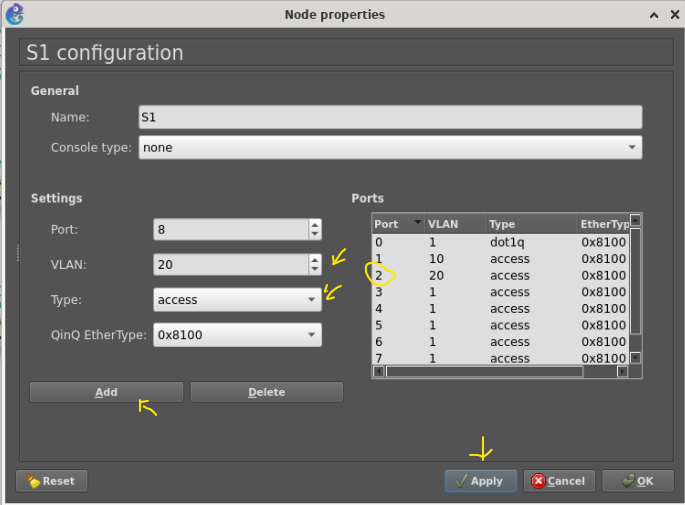
\includegraphics[width=0.6\textwidth]{../captures/03_vlan_graph_conf.png}
			\caption{Configuration des VLANs d'ID 10 et 20 sur le switch S1.}
			\label{fig:vlans-conf}
		\end{figure}
			\item \textbf{Configuration en ligne de commande \\}
				\begin{enumerate}
				\item \textbf{Définir le nom du switch et créer les VLANs :}
\begin{lstlisting}[language=bash]
	Switch> enable
	Switch# configure terminal
	Switch(config)# hostname S1
	S1(config)# vlan 10
	S1(config-vlan)# name VLAN_10
	S1(config-vlan)# exit
	S1(config)# vlan 20
	S1(config-vlan)# name VLAN_20
	S1(config-vlan)# exit	
\end{lstlisting}
	
	\item \textbf{Vérifier la création des VLAN :}
\begin{lstlisting}[language=bash]
	S1# show vlan brief
\end{lstlisting}	
	
	\item \textbf{Attribuer les interfaces aux VLAN 10 et 20 :}
\begin{lstlisting}[language=bash]
	S1(config)# interface e1
	S1(config-if)# switchport mode access
	S1(config-if)# switchport access vlan 10
	S1(config-if)# exit
	
	S1(config)# interface e2
	S1(config-if)# switchport mode access
	S1(config-if)# switchport access vlan 20
	S1(config-if)# exit
\end{lstlisting}		
	
	\item \textbf{Configurer l’interface \texttt{e0} en mode trunk pour la liaison avec le routeur R1 (et les autres switchs si nécessaire) :}
\begin{lstlisting}[language=bash]
	S1(config)# interface e0
	S1(config-if)# switchport trunk encapsulation dot1q  !ou bien : #switchport mode trunk
	S1(config-if)# switchport mode trunk
	S1(config-if)# switchport nonegotiate
	S1(config-if)# exit
\end{lstlisting}	
\end{enumerate}			
	\end{itemize}
\end{enumerate}
	
		
%------------------------------

\subsection{Routage inter-VLAN}

	\begin{enumerate}
		\item \textbf{Principe du Router-on-a-Stick}
	
Pour permettre la communication entre les différents VLANs sur chaque site, nous mettons en place une solution de type \textbf{router-on-a-stick}, qui consiste à utiliser un \textit{commutateur-routeur} configuré avec des \textbf{sous-interfaces VLAN} sur une interface physique unique.

Chaque routeur (R1 pour le site 1, R2 pour le site 2) utilise son interface \texttt{e1/1}, sur laquelle sont définies des sous-interfaces virtuelles associées à chaque VLAN. Chaque sous-interface est configurée avec :
\begin{itemize}
	\item une encapsulation VLAN via le protocole \texttt{dot1q} (IEEE 802.1Q),
	\item une adresse IP jouant le rôle de passerelle par défaut pour les hôtes du VLAN concerné,
	\item et une plage IP dédiée au réseau local du VLAN.
\end{itemize}

Cette solution est adaptée aux environnements de petite et 
moyenne taille. Dans une architecture à plus grande échelle, 
un commutateur de niveau 3 (Layer 3 switch) pourrait être 
préféré afin d’assurer le routage inter-VLAN directement au 
niveau du cœur de réseau.

Chaque sous-interface se voit attribuer une adresse IP qui joue le rôle de \textit{\textbf{passerelle par défaut}} pour les hôtes appartenant au VLAN correspondant.
%\bigskip

\begin{center}
	\resizebox{\textwidth}{!}{%
		\begin{tabular}{|c|c|c|c|c|c|}
			\hline
			\textbf{VLAN} & \textbf{Plage IP (Site 1)} & \textbf{Plage IP (Site 2)} & \textbf{Passerelle (Site 1)} & \textbf{Passerelle (Site 2)} & \textbf{Sous-interface} \\
			\hline
			VLAN\_10 & 192.168.1.0/27 & 192.168.2.0/27 & 192.168.1.1 & 192.168.2.1 & \texttt{e1/1.10} \\
			VLAN\_20 & 192.168.1.32/27 & 192.168.2.32/27 & 192.168.1.33 & 192.168.2.33 & \texttt{e1/1.20} \\
			VLAN\_31 & 192.168.1.64/29 & 192.168.2.64/29 & 192.168.1.65 & 192.168.2.65 & \texttt{e1/1.31} \\
			VLAN\_32 & 123.1.1.160/28 & 123.2.2.160/29 & 123.1.1.161 & 123.2.2.161 & \texttt{e1/1.32} \\
			\hline
		\end{tabular}
	}
\end{center}


	\item \textbf{Configuration des sous-interfaces sur le routeur R1}
\begin{enumerate}
	\item \textbf{Définition des sous-interfaces VLAN sur le routeur R1 \\} La configuration suivante permet de créer les différentes sous-interfaces sur le routeur R1 et d'associer chacune d'elles à un VLAN spécifique.
	
\begin{lstlisting}[language=bash,caption={Configuration des sous-interfaces sur R1}]
	enable
	configure terminal
	interface e1/1
	no shutdown
	
	interface e1/1.10
	encapsulation dot1Q 10
	ip address 192.168.1.1 255.255.255.224
	no shutdown
	exit
	
	interface e1/1.20
	encapsulation dot1Q 20
	ip address 192.168.1.33 255.255.255.224
	no shutdown
	exit
	
	interface e1/1.31
	encapsulation dot1Q 31
	ip address 192.168.1.65 255.255.255.248
	no shutdown
	exit
	
	interface e1/1.32
	encapsulation dot1Q 32
	ip address 123.1.1.161 255.255.255.240
	no shutdown
	exit
\end{lstlisting}
	
	\item \textbf{Vérification de la configuration }
	Une fois la configuration est appliquée, la commande suivante permet de vérifier les réseaux connus par le routeur :
\begin{lstlisting}[language=bash]
	R1# show ip route
	R1# show ip interface brief
\end{lstlisting}
	Cette commande affiche la table de routage et permet de confirmer que les différents sous-réseaux sont bien reconnus comme réseaux directement connectés
	\item \textbf{Sauvegarder la configuration du routeur \\}
	Afin de conserver la configuration après redémarrage du routeur, celle-ci est sauvegardée dans la mémoire non volatile:
	
\begin{lstlisting}[language=bash]
	R1# copy running-config startup-config
	ou bien une alternative : 
	R1#write memory
\end{lstlisting}	
	
\end{enumerate}

	\item \textbf{Configuration des sous-interfaces sur le routeur R2}
La configuration réalisée sur le routeur du site 2 suit la même logique que celle mise en place sur le site 1.  
Le routeur agit comme passerelle par défaut pour les différents VLAN du réseau local et assure le routage inter-VLAN grâce à l'utilisation de sous-interfaces associées à l'encapsulation \texttt{802.1Q}.

Chaque sous-interface est liée à un identifiant de VLAN spécifique et possède une adresse IP servant de passerelle pour les hôtes appartenant à ce réseau.

\begin{enumerate}
	
	\item \textbf{Définition des sous-interfaces VLAN sur le routeur R2}
\begin{lstlisting}[language=bash,caption={Configuration des sous-interfaces VLAN sur le routeur R2}]
	enable
	configure terminal
	
	interface e1/1
	no shutdown
	
	interface e1/1.10
	encapsulation dot1Q 10
	ip address 192.168.2.1 255.255.255.224
	no shutdown
	exit
	
	interface e1/1.20
	encapsulation dot1Q 20
	ip address 192.168.2.33 255.255.255.224
	no shutdown
	exit
	
	interface e1/1.31
	encapsulation dot1Q 31
	ip address 192.168.2.65 255.255.255.248
	no shutdown
	exit
	
	interface e1/1.32
	encapsulation dot1Q 32
	ip address 123.2.2.161 255.255.255.248
	no shutdown
	exit
\end{lstlisting}		
	
	\item \textbf{Vérification de la configuration}
	
	Une fois les sous-interfaces créées et les adresses IP attribuées, la table de routage du routeur peut être vérifiée afin de s'assurer que les différents réseaux VLAN sont correctement reconnus comme réseaux directement connectés.
	
\begin{lstlisting}[language=bash]
	R2# show ip route
	R2# show ip interface brief
\end{lstlisting}	
	
	\item \textbf{Sauvegarde de la configuration}
	
	Afin de conserver la configuration après redémarrage du routeur, celle-ci doit être enregistrée dans la mémoire non volatile :
	
\begin{lstlisting}[language=bash]
	R2# copy running-config startup-config
\end{lstlisting}	
	
	ou
	
\begin{lstlisting}[language=bash]
	R2# write memory
\end{lstlisting}	


\item La figure suivante illustre la configuration réalisée sur le routeur R1.
\medskip

\begin{figure}[H]
	\centering
	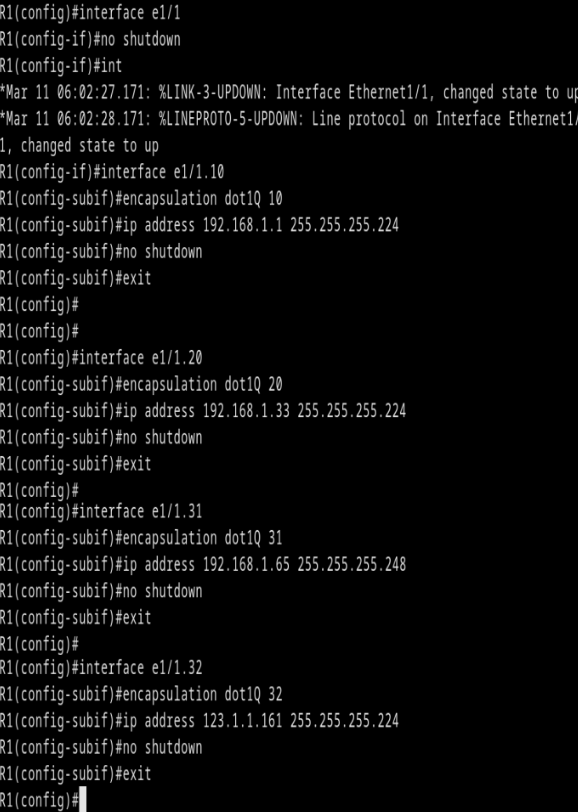
\includegraphics[width=0.9\linewidth]{../captures/04_vlan_ssInterfaceR1.png}
	\caption{Commandes de configuration des interfaces virtuelles sur le routeur R1 du site 1}
\end{figure}
\end{enumerate}
\end{enumerate}	
%-------------------------------

\subsection{Validation de la configuration}

	\begin{enumerate}
		\item \textbf{Vérification des interfaces et des VLAN}
	
	Les captures d’écran suivantes illustrent le résultat de la configuration des sous-interfaces : 

		\begin{enumerate}
			\item \textbf{Sur le routeur R1 (site 1) \\}
	
	\begin{figure}[H]
		\centering
		
		\begin{subfigure}{0.45\textwidth}
			\centering
			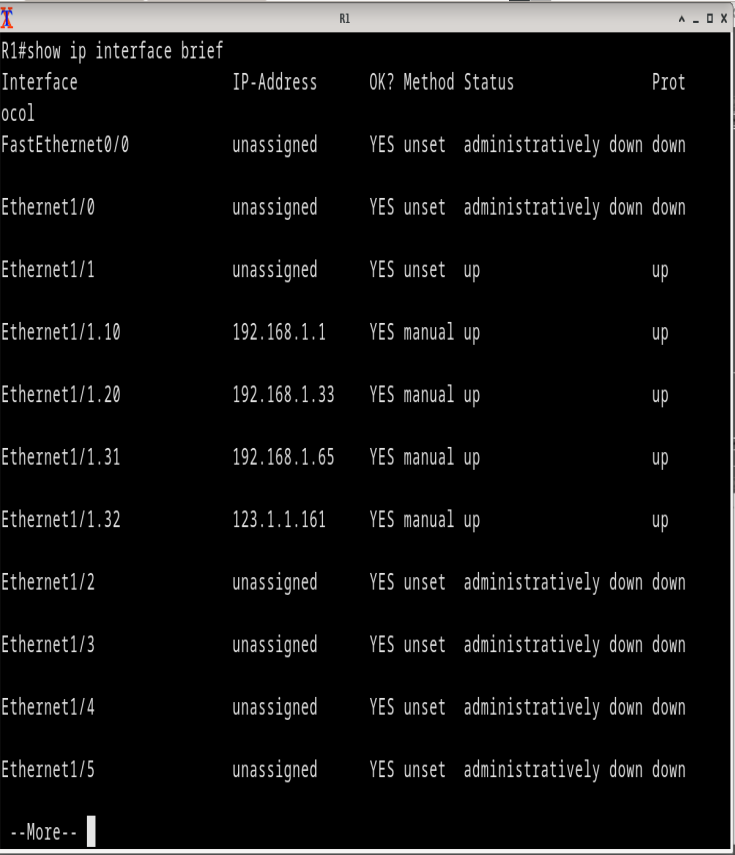
\includegraphics[width=\textwidth]{../captures/04_vlan_ssInterfaceR1_ShowInterfaceBrief.png}\\
			\caption{Etats des interfaces virtuelles sur le routeur R1 du site 1 }	
			\label{fig:etat-sous_interfaces_R1}
		\end{subfigure}
		\hfill
		\begin{subfigure}{0.45\textwidth}
			\centering
			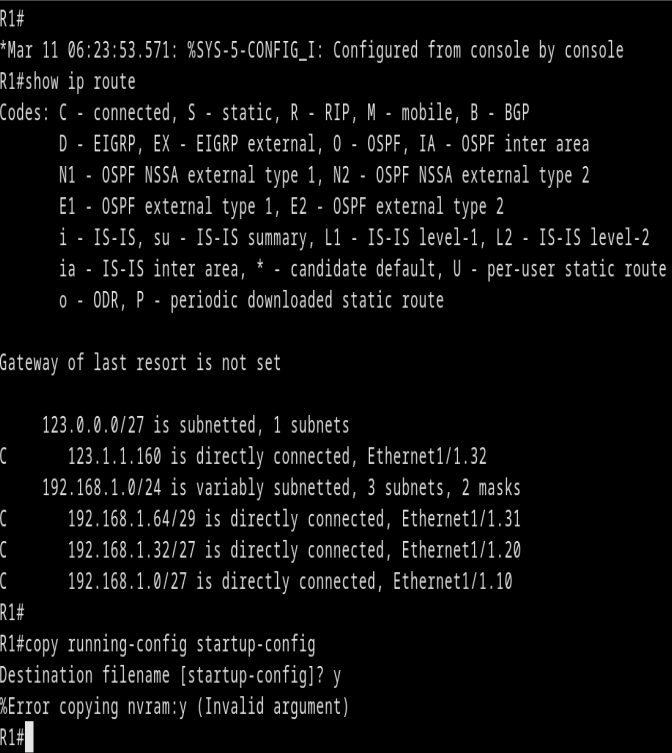
\includegraphics[width=\linewidth]{../captures/04_vlan_ssInterfaceR1_ShowIpRoute.png}
			\caption{Table de routage du routeur R1 après configuration des sous-interfaces VLAN}
			\label{fig:routing-r1}
		\end{subfigure}
		\caption{Configuration des sous_interfaces sur le routeur R1}
		\label{fig:reseau}
	\end{figure}

	\item \textbf{Sur le routeur R2 }

\begin{figure}[H]
	\centering
	
	\begin{subfigure}{0.45\textwidth}
		\centering
		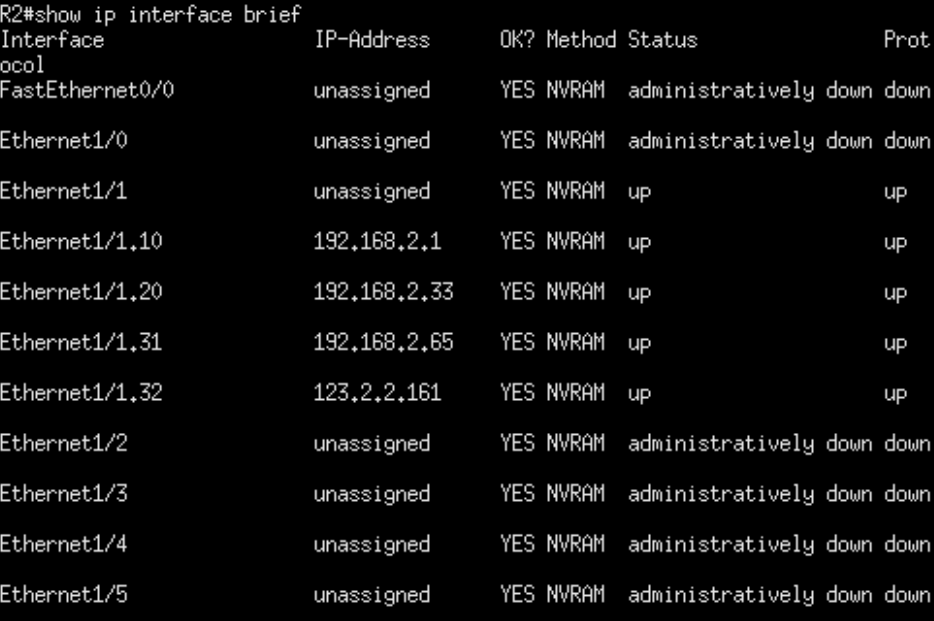
\includegraphics[width=\linewidth]{../captures/05_vlan_ssInterfaceR2_ShowInterfaceBrief.png}
		\caption{Etats des interfaces virtuelles sur le routeur R2 du site 2}
	\end{subfigure}
	\hfill
	\begin{subfigure}{0.45\textwidth}
		\centering
		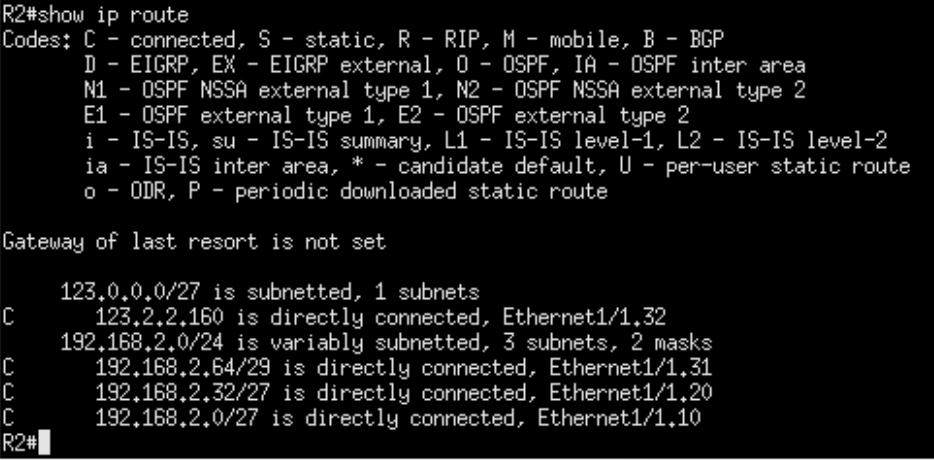
\includegraphics[width=\linewidth]{../captures/05_vlan_ssInterfaceR2_ShowIpRoute.png}
		\caption{Table de routage du routeur R2 après configuration}
	\end{subfigure}
	
	\caption{Configuration des sous-interfaces VLAN sur le routeur du site 2}
\end{figure}	
	
	Ces captures permettent d'observer plusieurs éléments importants :
	\begin{itemize}
		\item les sous-interfaces créées sur l'interface physique e1/1(e.g. \texttt{e1/1.10}, \texttt{e1/1.20}, etc.) ;
		\item les adresses IP attribuées à chacune d’elles, jouant le rôle de passerelle pour les VLANs ;
		\item l’état \texttt{up} des interfaces, indiquant leur bon fonctionnement ;
		\item les réseaux directement joignables à travers chaque sous-interface, permettant d’assurer le routage inter-VLAN.
	\end{itemize}
\end{enumerate}

	\item \textbf{Analyse des tables de routage}
		\begin{enumerate}
			\item \textbf{Site 1 :} 
	
	Dans la table de routage, les sous-réseaux 192.168.1.0/27, 192.168.1.32/27 et 192.168.1.64/29 apparaissent comme réseaux directement connectés (C). Chaque réseau est associé à une sous-interface spécifique du routeur (Ethernet1/1.10, Ethernet1/1.20 et Ethernet1/1.31).
	Le réseau 123.1.1.160/27, correspondant à l’infrastructure publique, est également directement connecté via l’interface Ethernet1/1.32.
	Cette configuration permet d'assurer la connectivité avec l'infrastructure publique du site.
	Enfin, l'absence de gateway of last resort indique qu’aucune route par défaut n’a encore été configurée à ce stade de l’implémentation.


		\item textbf{Site 2 :}

L'analyse de la table de routage montre que les réseaux suivants sont directement connectés au routeur :

\begin{itemize}
	\item \texttt{192.168.2.0/27} : VLAN administratif
	\item \texttt{192.168.2.32/27} : VLAN développeurs
	\item \texttt{192.168.2.64/29} : VLAN serveurs intranet
	\item \texttt{123.2.2.160/29} : réseau des serveurs publics
\end{itemize}

Chaque réseau est associé à une sous-interface spécifique du routeur (\texttt{Ethernet1/1.X}), permettant d'assurer le routage inter-VLAN au sein du site 2.
	\end{enumerate}
Comme pour le site 1, l'absence de \textit{gateway of last resort} indique qu'aucune route par défaut n'a encore été définie à ce stade de la configuration. Cette route sera ajoutée ultérieurement afin d'assurer l'accès aux réseaux externes et à Internet.

%--------------------------------------------

Afin de valider le fonctionnement du routage inter-VLAN au niveau des couches basses du modèle réseau, une analyse du trafic a été réalisée à l’aide de l’outil \textbf{Wireshark}.


\item \textbf{Tests de connectivité entre les différents équipements}

Afin de valider le bon fonctionnement de l’architecture réseau mise en place, des tests de connectivité ont été réalisés entre les différents équipements à l’aide de la commande \texttt{ping}. 

Ces tests reposent sur le protocole ICMP (\textit{Internet Control Message Protocol}), permettant de vérifier l’accessibilité entre des hôtes situés dans des VLANs distincts.

\medskip
\begin{enumerate}
	\item \textbf{Tests de connectivité ICMP (ping)}

Des requêtes ICMP ont été émises entre plusieurs VLANs d’un même site, notamment :
\begin{itemize}
	\item entre le VLAN\_10 (Administratif) et le VLAN\_20 (Développeurs),
	\item entre les VLANs utilisateurs (VLAN\_10, VLAN\_20) et les VLANs serveurs (VLAN\_31 et VLAN\_32).
\end{itemize}

\medskip

La figure suivante illustre un exemple de test de connectivité entre deux hôtes appartenant à des VLANs différents.

\begin{figure}[H]
	\centering
	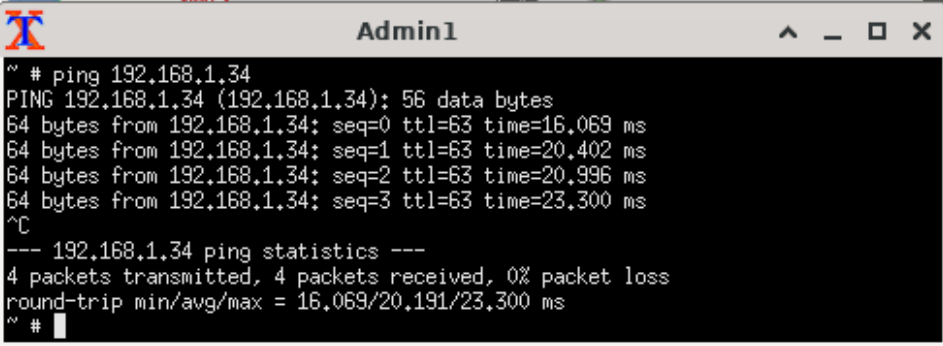
\includegraphics[width=0.9\textwidth]{../captures/06_ping_vlan10_vers_vlan20.png}
	\caption{Test de connectivité ICMP entre VLAN\_10 et VLAN\_20}
	\label{fig:ping_inter_vlan}
\end{figure}

Les résultats obtenus montrent que :
\begin{itemize}
	\item les paquets ICMP sont correctement transmis entre les différents VLANs ;
	\item aucune perte de paquets n’est observée ;
	\item les temps de réponse sont cohérents avec une communication locale.
\end{itemize}

Ces observations confirment le bon fonctionnement du routage inter-VLAN assuré par les sous-interfaces du routeur.

\medskip

	\item \textbf{Analyse du trafic avec Wireshark}

Afin d’approfondir la validation du fonctionnement réseau, une analyse du trafic a été réalisée à l’aide de l’outil \textbf{Wireshark}. Cette analyse permet d’observer les échanges au niveau des couches basses du modèle OSI.

\medskip

Une capture du trafic ICMP a été effectuée lors de l’émission d’un \texttt{ping} entre deux VLANs distincts. Cette capture a été réalisée sur le lien \textit{trunk} reliant le commutateur au routeur du site, transportant les trames des différents VLAN via le protocole \texttt{IEEE 802.1Q}.

Le filtre suivant a été utilisé dans Wireshark afin d’isoler les paquets ICMP :
\texttt{icmp}

Pour observer les VLAN :
\texttt{vlan.id == 10 || vlan.id == 20}

\begin{figure}[H]
	\centering
	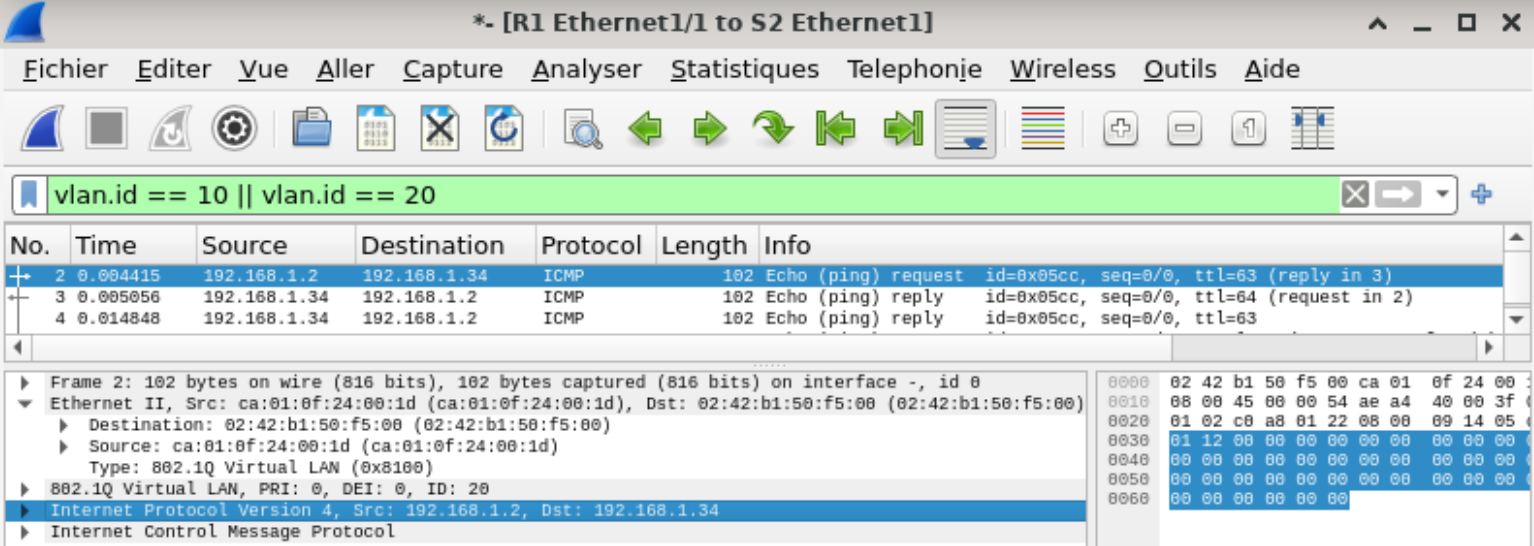
\includegraphics[width=0.98\textwidth]{../captures/06_wireshark_icmp_vlan.png}
	\caption{Capture Wireshark du trafic ICMP entre deux VLANs}
	\label{fig:wireshark_icmp}
\end{figure}

L’analyse des paquets capturés met en évidence les éléments suivants :

\begin{itemize}
	\item présence de requêtes ICMP de type \texttt{Echo Request} et réponses \texttt{Echo Reply} ;
	\item modification des adresses MAC à chaque saut (passage par le routeur) ;
	\item conservation des adresses IP source et destination, confirmant le routage de niveau 3 ;
	\item absence de marquage VLAN visible sur l’hôte, celui-ci étant géré au niveau du trunk entre le switch et le routeur.
\end{itemize}

\medskip

Ces observations confirment que :
\begin{itemize}
	\item le routage inter-VLAN est correctement assuré par le routeur (\textit{router-on-a-stick}) ;
	\item les communications respectent le modèle en couches (L2 pour la commutation, L3 pour le routage) ;
	\item l’infrastructure réseau est fonctionnelle et cohérente avec le plan d’adressage défini.
	\item des trames Ethernet encapsulant des balises VLAN (\texttt{802.1Q}) identifiant les réseaux logiques traversés.
\end{itemize}
\end{enumerate}

\item \textbf{Interprétation des résultats}

Les tests de connectivité ainsi que l’analyse des captures réseau permettent de valider plusieurs points essentiels de l’architecture :

\begin{itemize}
	\item le bon fonctionnement du routage inter-VLAN via le mécanisme de \textit{router-on-a-stick} ;
	\item la correcte segmentation logique des réseaux grâce aux VLANs ;
	\item la cohérence entre la configuration théorique (plan d’adressage) et le comportement réel du réseau ;
	\item la fiabilité des communications entre les différents équipements du site.
\end{itemize}
\end{enumerate}
Ces résultats confirment que l’infrastructure réseau est opérationnelle et conforme aux exigences de segmentation, de communication et de performance définies en phase de conception.

%%%%%%%%%%%%%%%%%%%%%%%%%%%%%%%%%%%%%%%%%%%%%%%%%%%%%%%%%%%%%%%%%%%%%

\section{Mise en place des services réseau : DHCP, NAT et ACL}
Ce chapitre présente la mise en oeuvre des principaux services réseau nécessaires au bon fonctionnement de l’architecture multi-sites : l’attribution des adresses IP (DHCP), la traduction d’adresses (NAT) et le contrôle des flux (ACL).  
L’objectif est d’assurer à la fois la connectivité, la sécurité et la maîtrise des échanges entre les différents VLANs et avec Internet.

%=================================================
	\subsection{Attribution dynamique des adresses IP : DHCP}
	
		\begin{enumerate}
			\item \textbf{Choix du mode d’adressage}
		Dans l’architecture proposée, chaque site est segmenté en plusieurs VLANs correspondant à différents usages (administratif, développement, serveurs).
		
		Le choix du mode d’attribution des adresses IP est le suivant :
		
			\begin{itemize}
				\item \textbf{DHCP} pour les postes utilisateurs (VLAN\_10, VLAN\_20)
				\item \textbf{Adresses statiques} pour les serveurs
			\end{itemize}
		
		Les serveurs internes (VLAN\_31) peuvent fonctionner en DHCP, mais une adresse statique est recommandée pour garantir la stabilité des services.  
		
		Les serveurs publics (VLAN\_32) doivent impérativement disposer d’adresses IP fixes afin d’être accessibles depuis Internet.
	
		\item \textbf{Implémentation du service DHCP}
	
	Le protocole DHCP a été mis en place afin d’automatiser l’attribution des adresses IP aux hôtes des différents VLANs.
	
	La mise en place du DHCP est implémentée sur les routeurs, en mode de configuration globale (configure terminal) et elle repose sur les étapes suivantes: 
	
		\begin{enumerate}
			\item  \textbf{Création des pools DHCP}
			
		Chaque VLAN utilisateur dispose d'un pool dédié. CI-dessous l'implémentation du pool poolVLAN\_10 pour le VLAN\_10 administratif (idem pour le VLAN\_20) : 
		\begin{verbatim}
			ip dhcp pool poolVLAN_10             ! Active le service DHCP
			network 192.168.1.0 255.255.255.224  ! Associe un sous-réseau au pool
			default-router 192.168.1.1   ! Définit l’adresse de la passerelle pour le VLAN
			lease 7   ! Durée du bail : 7 jours (ou lease 12 pour 12h)
		\end{verbatim}

		\item \textbf{Exclusion d’adresses}
		
		Certaines adresses sont exclues pour des équipements critiques : 
		\begin{verbatim}
			ip dhcp excluded-address 192.168.1.1 192.168.1.5 
		\end{verbatim}
		
		\item \textbf{Relais DHCP}
		
		\begin{itemize}
			\item Le service DHCP est directement implémenté sur les routeurs de chaque site. Ainsi, aucun mécanisme de relai DHCP n’est nécessaire, les requêtes étant traitées localement.
			
			\item  Dans le cas où le serveur DHCP était centralisé, les requêtes sont relayées via :
			\begin{verbatim}
				ip helper-address @ip\_serveur\_DHCP
			\end{verbatim}
		\end{itemize}
	
	\item \textbf{Mise en pratique}
	
	La figure~\ref{fig:dhcp_impl} présente les différentes configurations réalisées pour activer le service DHCP :
	
	\begin{itemize}
		\item sur le routeur R1 du site 1 ;
		\item sur le routeur R2 du site 2 ;
		\item sur un hôte du VLAN Administratif configuré pour obtenir automatiquement une adresse IP.
	\end{itemize}
	
	\begin{figure}[H]
		\centering
		\begin{subfigure}[b]{0.75\textwidth}
			\centering
			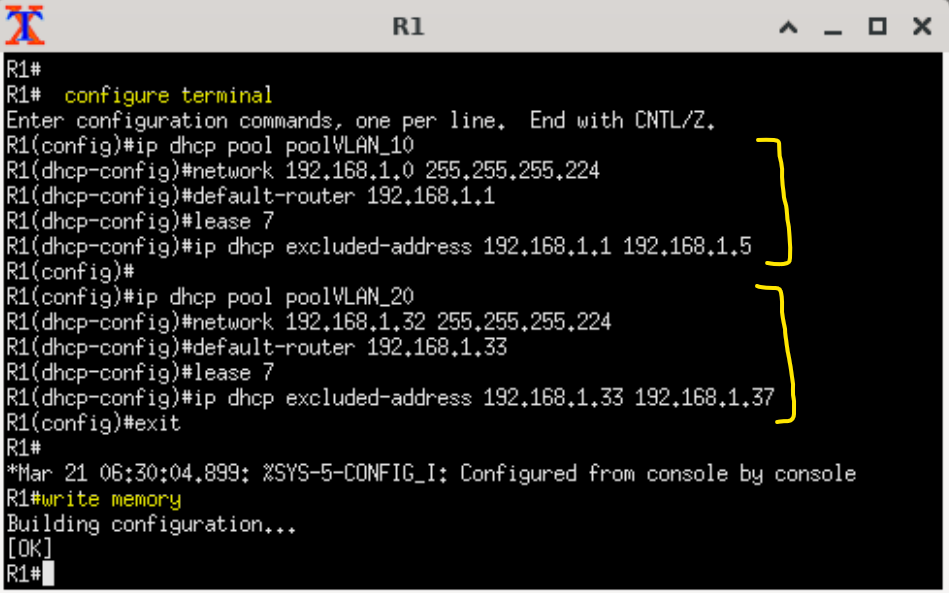
\includegraphics[width=\textwidth]{../captures/07_dhcp_R1_impl.png}
			\caption{Configuration DHCP sur R1}
		\end{subfigure}
		\hfill
		\begin{subfigure}[b]{0.75\textwidth}
			\centering
			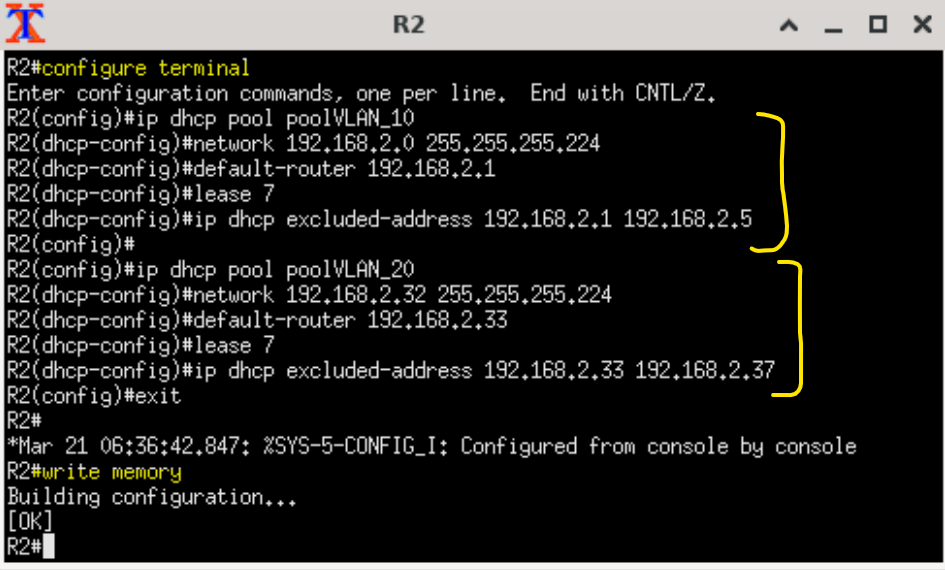
\includegraphics[width=\textwidth]{../captures/07_dhcp_R2_impl.png}
			\caption{Configuration DHCP sur R2}
		\end{subfigure}
		\hfill
		\begin{subfigure}[b]{0.75\textwidth}
			\centering
			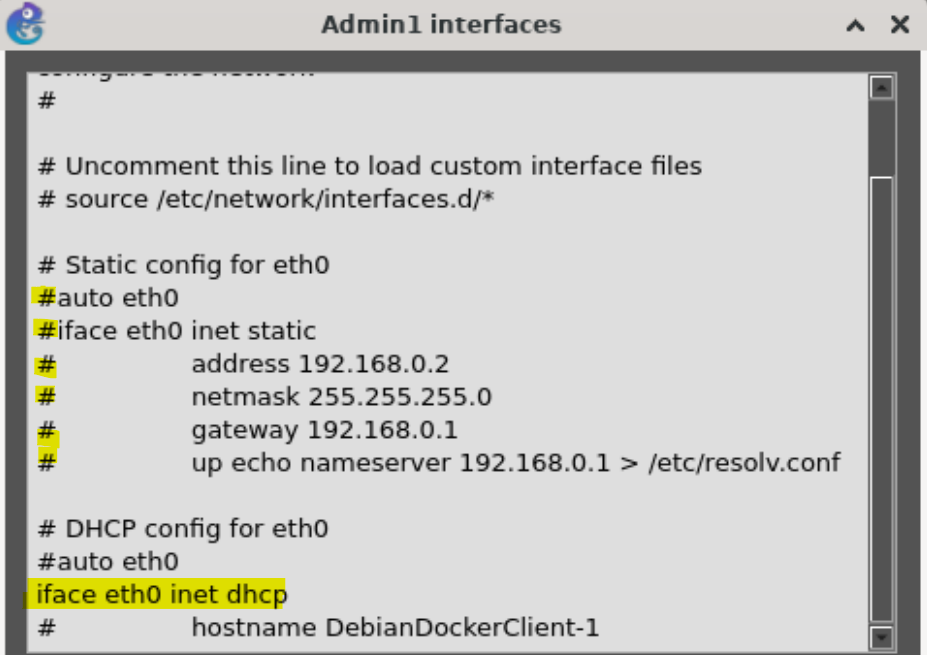
\includegraphics[width=\textwidth]{../captures/07_dhcp_sur_hotes.png}
			\caption{Configuration DHCP sur un hôte}
		\end{subfigure}
		\caption{Implémentation du service DHCP sur les routeurs et un hôte client}
		\label{fig:dhcp_impl}
	\end{figure}	
\end{enumerate}	
\end{enumerate}	
%	\subsection{Problèmes rencontrés}
%	Les requêtes DHCP seront initialement bloquées par les ACL.  
%	La solution a consisté à autoriser explicitement les flux UDP (ports 67 et 68)(voir \label{DHCP_ACL}).

	
	\subsection{Validation du DHCP}	
	Une fois le service configuré, les commandes de supervision permettent de vérifier son bon fonctionnement sont les suivantes.
	
	\begin{itemize}
		\item \texttt{show ip dhcp pool} : affiche les pools configurés ainsi que le nombre d’adresses disponibles et utilisées ;
		\item \texttt{show ip dhcp binding} : liste les adresses IP attribuées aux clients (baux actifs).
	\end{itemize}
		La figure~\ref{fig:dhcp_show} illustre les résultats de ces commandes :	
	\begin{figure}[H]
		\centering
		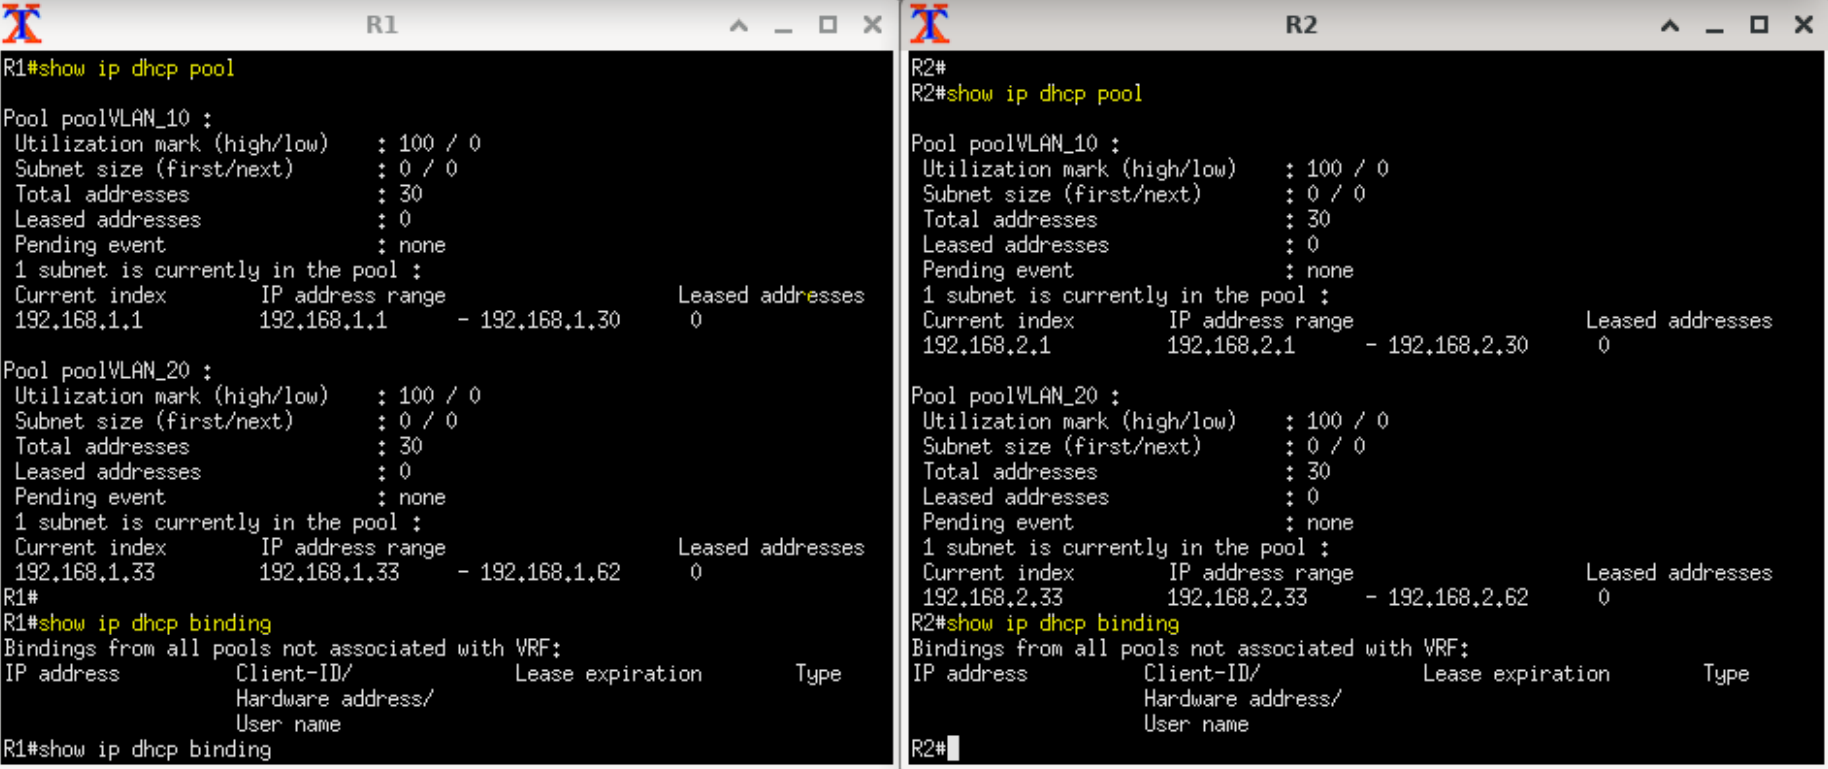
\includegraphics[width=1\textwidth]{../captures/07_dhcp_show.png}
		\caption{Affichage des pools DHCP et des baux actifs}
		\label{fig:dhcp_show}
	\end{figure}
	
	\subsection{Analyse du fonctionnement du DHCP}
	
	Enfin, la figure~\ref{fig:dhcp_resultats} présente les résultats expérimentaux confirmant le bon fonctionnement du service DHCP :
	
	\begin{figure}[H]
		\centering
		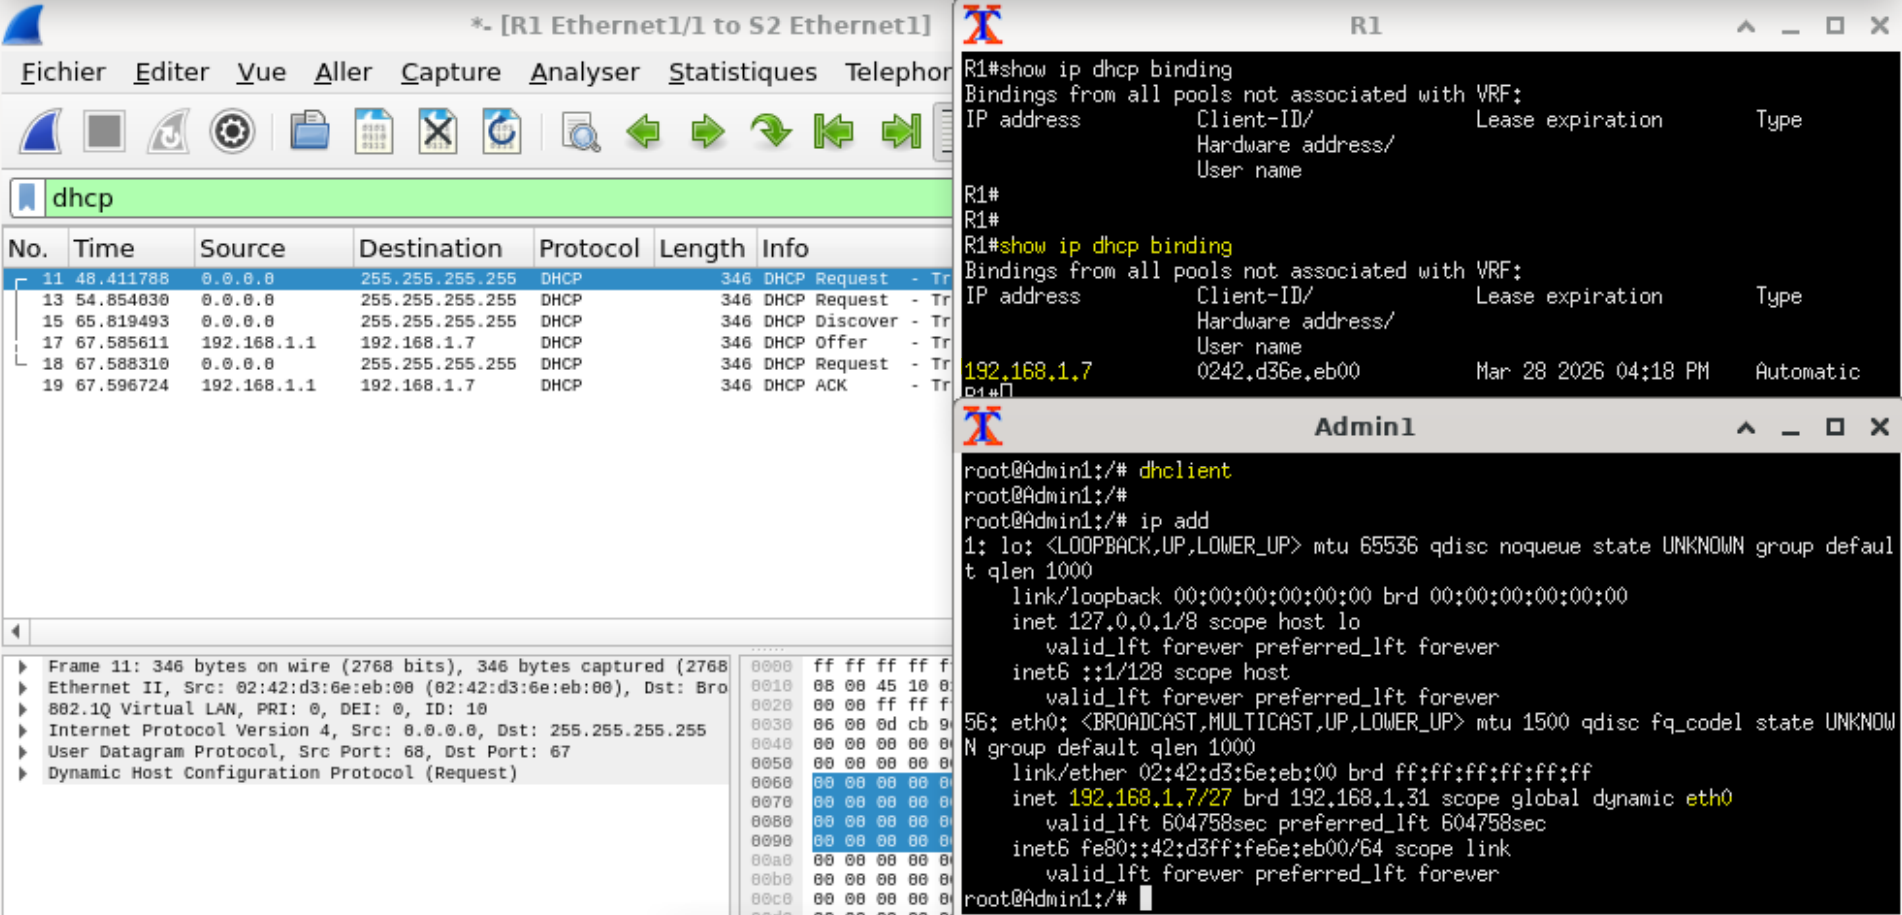
\includegraphics[width=1\textwidth]{../captures/07_dhcp_resultats.png}
		\caption{Résultats de l’attribution DHCP : capture réseau, baux et configuration côté client}
		\label{fig:dhcp_resultats}
	\end{figure}
	
	\medskip
	Les captures réalisées à l’aide de Wireshark mettent en évidence la séquence complète d’attribution d’une adresse IP via le protocole DHCP, connue sous l’acronyme DORA (Discover, Offer, Request, Acknowledgment).
	
	\begin{itemize}
		\item \textbf{DHCP Discover} : 
		Le client, ne disposant d’aucune configuration IP initiale, envoie une requête de découverte en broadcast (adresse de destination 255.255.255.255). 
		Ce message permet de localiser les serveurs DHCP disponibles sur le réseau. 
		À ce stade, le client utilise l’adresse IP source 0.0.0.0, car il ne possède pas encore d’adresse valide.
		
		\item \textbf{DHCP Offer} : 
		Le serveur DHCP répond par un message DHCPOFFER, contenant une proposition d’adresse IP ainsi que les paramètres réseau associés (masque de sous-réseau, passerelle par défaut, durée du bail, etc.). 
		Cette réponse est généralement envoyée en broadcast, car le client n’a pas encore configuré son interface réseau.
		
		\item \textbf{DHCP Request} : 
		Le client sélectionne l’une des offres reçues et envoie un message DHCPREQUEST pour indiquer son acceptation. 
		Ce message est également diffusé en broadcast afin d’informer les autres serveurs DHCP que leurs offres ne sont pas retenues.
		
		\item \textbf{DHCP ACK (Acknowledgment)} : 
		Le serveur confirme l’attribution de l’adresse IP à l’aide d’un message DHCPACK. 
		Ce message final contient l’ensemble des paramètres réseau nécessaires à la configuration du client, qui peut alors initialiser son interface avec l’adresse IP attribuée.
	\end{itemize}
	
	\medskip
	
	\noindent
	L’observation de cette séquence complète dans les captures Wireshark confirme le bon fonctionnement du service DHCP. Elle montre que les requêtes des clients sont correctement relayées et traitées, et que les adresses IP sont attribuées de manière dynamique conformément à la configuration des pools DHCP définis sur les routeurs.
%\end{enumerate}

%%%%%%%%%%%%%%%%%%%%%%%%%%%%%%%%%%%%%%%%%%%%%%%%%%%%%%%%%%%%%%%%%%%%%

\subsection{Traduction d’adresses : NAT}

\subsubsection{Besoins et contraintes}

Les VLANs privés doivent accéder à Internet, tandis que les serveurs publics doivent être directement accessibles.

Les besoins sont :
\begin{itemize}
	\item NAT pour les VLAN privés (10, 20, 31)
	\item Accès direct pour VLAN\_32 (IP publiques)
\end{itemize}

\subsubsection{Découpage des plages publiques}

Chaque site dispose d’un bloc d’adresses IPv4 publiques en /27, subdivisé selon les besoins en sous-réseaux dédiés aux serveurs publics, à la liaison WAN avec l’opérateur et au pool NAT, voir le tableau~\ref{tab:decoupage_plages_publiques}.


\subsubsection{Configuration NAT}

Les configurations NAT mises en place sur les routeurs R1 (Site 1) et R2 (Site 2) reposent sur le principe du NAT dynamique avec surcharge (PAT). Le tableau~\ref{tab:nat_configuration} présente les différentes étapes de configuration.
\begin{landscape}
	\begin{table}[H]
		\centering
		\caption{Découpage des plages d’adresses publiques pour les deux sites}
		\renewcommand{\arraystretch}{1.2}
		\begin{tabular}{|c|c|c|c|p{10cm}|}
			\hline
			\textbf{Site} & \textbf{Usage} & \textbf{Sous-réseau} & \textbf{Plage IP} & \textbf{Description} \\
			\hline
			
			\multirow{3}{*}{Site 1} 
			& VLAN\_32 & 123.1.1.160/28 & 123.1.1.161 -- 123.1.1.174 & Serveurs publics (14 IP utilisables) \\
			\cline{2-5}
			& WAN & 123.1.1.176/31 & 123.1.1.176 -- 123.1.1.177 & Liaison point-à-point avec l’opérateur \\
			\cline{2-5}
			& NAT & 123.1.1.178/27 & 123.1.1.178 -- 123.1.1.190 & Pool d’adresses publiques pour le NAT dynamique \\
			
			\hline
			\hline
			
			\multirow{3}{*}{Site 2} 
			& VLAN\_32 & 123.2.2.160/29 & 123.2.2.161 -- 123.2.2.166 & Serveurs publics (6 IP utilisables) \\
			\cline{2-5}
			& WAN & 123.2.2.168/31 & 123.2.2.168 -- 123.2.2.169 & Liaison point-à-point avec l’opérateur \\
			\cline{2-5}
			& NAT & 123.2.2.170/27 & 123.2.2.170 -- 123.2.2.190 & Pool d’adresses publiques pour le NAT dynamique \\
			
			\hline
		\end{tabular}
		\label{tab:decoupage_plages_publiques}
	\end{table}
	
\begin{table}[H]
	\centering
	\caption{Configuration du NAT dynamique (PAT) sur les routeurs -en mode config-}
	\renewcommand{\arraystretch}{1.3}
	\begin{tabular}{|p{3cm}|p{10.3cm}|p{10.3cm}|}
		\hline
		\textbf{Étape} & \textbf{R1 (Site 1)} & \textbf{R2 (Site 2)} \\
		\hline
		
		Définition des réseaux internes (ACL) 
		& 
		\texttt{access-list 1 permit 192.168.1.0 0.0.0.31} \newline 
		\texttt{access-list 1 permit 192.168.1.32 0.0.0.31} \newline 
		\texttt{access-list 1 permit 192.168.1.64 0.0.0.7}
		&
		\texttt{access-list 2 permit 192.168.2.0 0.0.0.31} \newline
		\texttt{access-list 2 permit 192.168.2.32 0.0.0.31} \newline 
		\texttt{access-list 2 permit 192.168.2.64 0.0.0.7}
		\\
		\hline
		
		Création du pool NAT 
		&
		\small{\texttt{ip nat pool NAT\_POOL\_SITE1} %\newline
		\texttt{123.1.1.178 123.1.1.190} %\newline
		\texttt{netmask 255.255.255.224}}
		&
		\small{\texttt{ip nat pool NAT\_POOL\_SITE2} %\newline
		\texttt{123.2.2.170 123.2.2.190} %\newline
		\texttt{netmask 255.255.255.224}}
		\\
		\hline
		
		Activation du NAT (PAT)
		&
		\texttt{ip nat inside source list 1} %\newline
		\texttt{pool NAT\_POOL\_SITE1 overload}
		&
		\texttt{ip nat inside source list 2} %\newline
		\texttt{pool NAT\_POOL\_SITE2 overload}
		\\
		\hline
		
		Interfaces internes (inside)
		&
		\texttt{e1/1.10, e1/1.20, e1/1.31}
		&
		\texttt{e1/1.10, e1/1.20, e1/1.31}
		\\
		& Ex. : \newline
		interface e1/1.10 \newline
		ip nat inside & (idem)\\
		\hline
		
		Interface externe (outside)
		&
		\texttt{f0/0} (idem)
		&
		\texttt{f0/0} (idem)
		\\
		\hline
		
	\end{tabular}
	\label{tab:nat_configuration}
\end{table}
\end{landscape}
\medskip

\noindent
Les serveurs du VLAN\_32 ne nécessitent pas de traduction d’adresses (NAT), car ils disposent déjà d’adresses IP publiques. Ils sont donc directement accessibles depuis Internet, sous réserve de règles de routage et de filtrage appropriées.

\textbf{Remarque :} Il est important de noter que les listes de contrôle d’accès (ACL) utilisées dans la configuration du NAT ne remplissent pas un rôle de filtrage du trafic. Elles servent uniquement à identifier les réseaux internes dont les adresses doivent être traduites. Contrairement aux ACL de sécurité, ces règles ne sont pas appliquées directement sur les interfaces du routeur, mais sont utilisées comme critère de sélection dans le processus de traduction d’adresses.

\subsubsection{Topologie nécessaire pour réaliser un test de validation du NAT}
Afin de valider le bon fonctionnement du mécanisme de traduction d’adresses (NAT), une simulation d’accès à Internet a été mise en place dans l’environnement GNS3. Pour cela, un routeur a été ajouté dans la zone opérateur afin de représenter une sortie vers l’extérieur, figure~\ref{fig:nat_topologie}. Ce routeur est interconnecté avec les routeurs des deux sites via des liaisons point-à-point, permettant d’assurer la connectivité entre les réseaux internes et l’environnement simulé.
	
\begin{figure}[H]
	\centering
	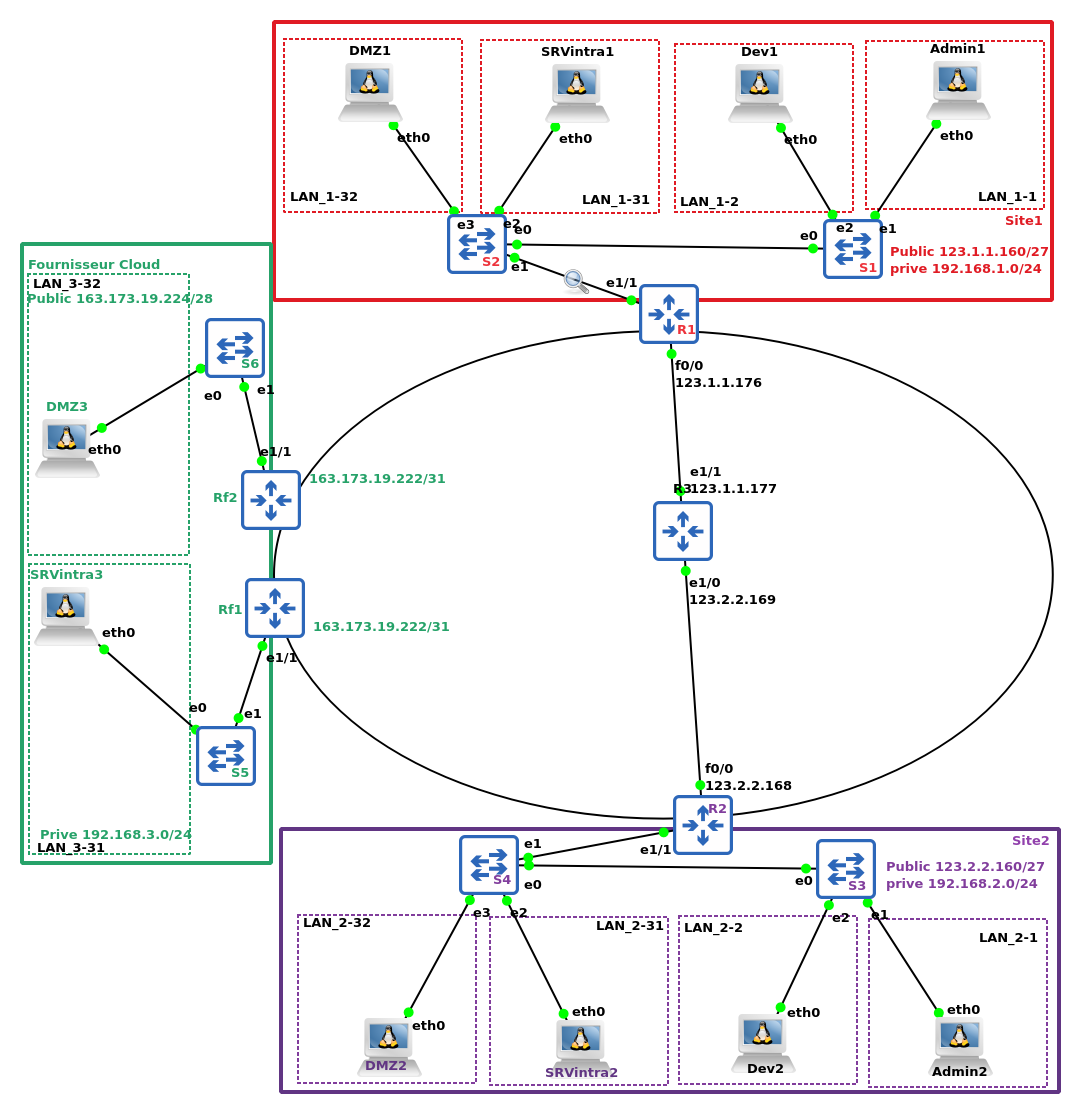
\includegraphics[width=0.8\textwidth]{../captures/08_nat_topologie.png}
	\caption{Topologie de test avec simulation d’Internet via le routeur opérateur}
	\label{fig:nat_topologie}
\end{figure}

Les caractéristiques des interconnexions entre les routeurs sont résumées dans le tableau~\ref{tab:liaisons_operateur}.

\begin{table}[H]
	\centering
	\renewcommand{\arraystretch}{1.3}
	\begin{tabular}{|c|c|c|c|c|}
		\hline
		\textbf{Site} & \textbf{Interface R1/2} & \textbf{Interface R3 Op} & \textbf{Réseau} & \textbf{Adresses IP} \\
		\hline
		Site 1 & f0/0 (R1) & e1/1 (Opérateur) & 123.1.1.176/31 & 123.1.1.176 / 123.1.1.177 \\
		\hline
		Site 2 & f0/0 (R2) & e0/1 (Opérateur) & 123.2.2.168/31 & 123.2.2.168 / 123.2.2.169 \\
		\hline
	\end{tabular}
	\caption{Liaisons point-à-point entre les routeurs des sites et le routeur opérateur}
	\label{tab:liaisons_operateur}
\end{table}
	
\subsubsection{Validation du fonctionnement du NAT}

La validation a été réalisée à partir d’un hôte du réseau interne (poste administrateur), en initiant un ping vers l’adresse \texttt{8.8.8.8}. Lors de cette opération, l’activation du mode debug sur le routeur R1 (\texttt{debug ip nat}) a permis d’observer en temps réel la traduction d’adresse, avec le message indiquant le passage de l’adresse source privée \texttt{192.168.1.6} vers une adresse publique du pool NAT, par exemple \texttt{123.1.1.179}. Cette correspondance confirme que le trafic issu du réseau interne est correctement traduit avant d’être transmis vers l’extérieur. Ainsi, la combinaison des tests de connectivité et des traces de débogage atteste du bon fonctionnement du NAT dynamique avec surcharge (PAT), validant la configuration mise en place dans cette architecture réseau. Le tableau~\ref{tab:validation_nat} résume les étapes mises en œuvre et la figure~\ref{tab:validation_nat} illustre les résultats obtenus.

\begin{table}[H]
	\centering
	\renewcommand{\arraystretch}{1.3}
	\begin{tabular}{|p{3.5cm}|c|l|}
		\hline
		\textbf{Étape} & Commande & \textbf{Description} \\
		\hline
		Simulation & R1-R3-R2 & Ajout d’un routeur dans la zone \\
		 d’Internet & & opérateur afin de simuler une \\
		  & & connectivité externe. \\
		\hline
		
		Configuration  & interface loopback0 & Création d’une interface loopback\\
		d’une destination & ip address 8.8.8.8 255.255.255.255 & sur le routeur opérateur avec \\
		distante (sur R3)&  & l’adresse \texttt{8.8.8.8/32}.\\
		\hline
		
		Routage sortant & ip route 0.0.0.0 0.0.0.0 123.1.1.177 & Configuration d’une route par  \\
		(R1) & & défaut sur R1 (.177 est l'adresse\\
		& &  du prochain saut).\\
		\hline
		
		Routage retour& \texttt{ip route 123.1.1.160 } & Ajout d’une route  \\
		 (sur R3) & \texttt{255.255.255.224 123.1.1.176} & vers le réseau interne. \\
		\hline
		Test de connecti- & \texttt{ping 8.8.8.8} & Envoi d’un ping depuis un hôte \\
		 vité& &  interne (192.168.1.6) vers \texttt{8.8.8.8}. \\
		\hline
		
		Activation du  & debug ip nat & Pour observer la traduction \\
		 debug NAT sur R1 & &  d’adresse en temps réel. \\
		\hline
		
		Résultat & show ip nat translations & \texttt{NAT:s=192.168.1.6→123.1.1.179} \\
		& & Traduction observée confirmant \\
		 & & le bon fonctionnement du NAT. \\
		\hline
		
	\end{tabular}
	\caption{Étapes de validation du NAT dans l’architecture réseau}
	\label{tab:validation_nat}
\end{table}
	
	\textbf{Remarque :}Les entrées de la table NAT étant dynamiques et temporaires, leur observation nécessite la génération d’un trafic continu. Par ailleurs, le routage côté opérateur doit être configuré vers les adresses publiques traduites et non vers les adresses privées internes.
	\begin{figure}[H]
		\centering
		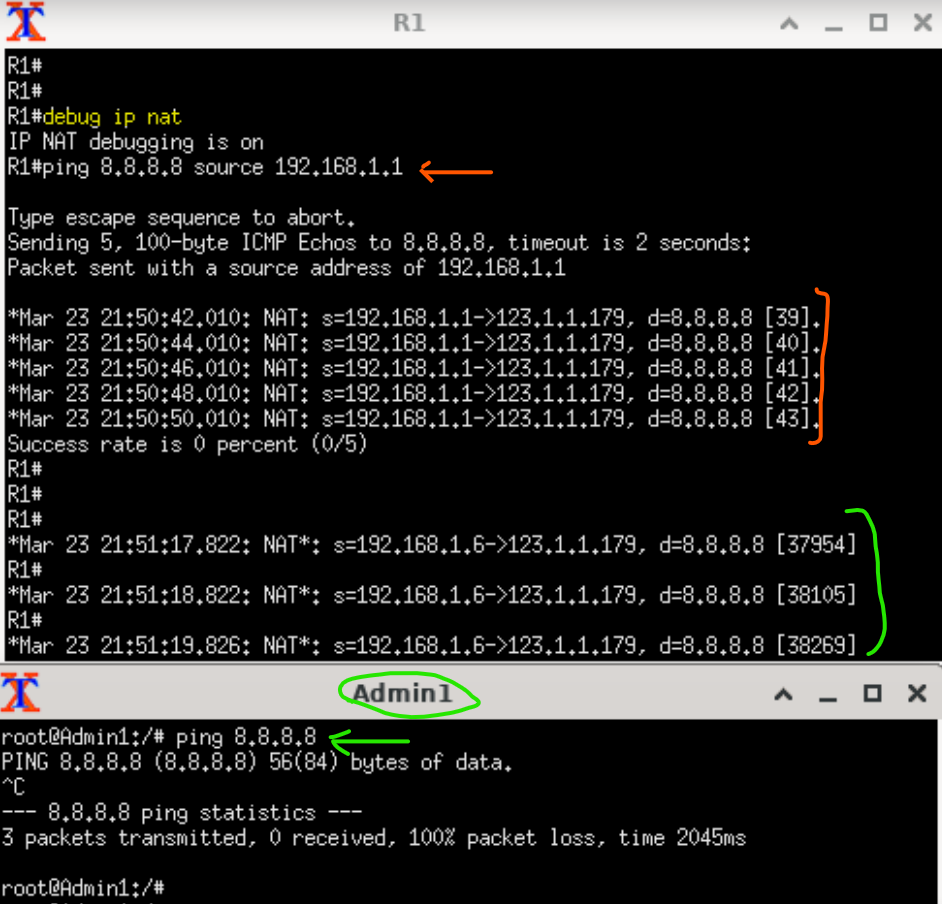
\includegraphics[width=0.9\textwidth]{../captures/08_nat_debug.png}
		\caption{Observation de la traduction d’adresse via la commande \texttt{debug ip nat} sur R1 -à droite- et le test de connectivité depuis un hôte interne vers l’adresse externe simulée (8.8.8.8) -à gauche-.}
		\label{fig:nat_debug}
	\end{figure}
\newpage
%%%%%%%%%%%%%%%%%%%%%%%%%%%%%%%%%%%%%%%%%%%%%%%%%%%%%%%%%%%%%%%%%%%%%
\subsection{Contrôle d’accès : ACL}

%\subsection{Analyse des contraintes}
\subsubsection{Expression des besoins en matière d’ACL de sécurité}

Les contraintes de sécurité définies pour l’architecture réseau sont traduites en règles de filtrage (ACL). Le tableau~\ref{tab:besoins_acl} synthétise les besoins en termes de contrôle des flux entre les différents VLANs et vers Internet.

\begin{table}[H]
	\centering
	\renewcommand{\arraystretch}{1.3}
	\begin{tabular}{|c|c|c|p{6cm}|}
		\hline
		\textbf{Source} & \textbf{Destination} & \textbf{Action} & \textbf{Justification} \\
		\hline
		VLAN\_10 (Admin) & VLAN\_20 (Dev) & Refuser & Isolation entre départements pour des raisons de sécurité \\
		\hline
		VLAN\_20 (Dev) & VLAN\_10 (Admin) & Refuser & Isolation bidirectionnelle des flux \\
		\hline
		
		VLAN\_31  & VLAN\_32  & Refuser & Séparation des environnements \\
		(Serveurs internes) & (Serveurs publics) &  & interne et exposé  \\
		\hline
		
		VLAN\_32  & VLAN\_31  & Refuser & Protection des serveurs internes \\
		(Serveurs publics) & (Serveurs internes) &  & Protection des serveurs internes \\
		\hline
		
		VLAN\_10 & VLAN\_31 & Autoriser & Accès des administratifs aux services internes \\
		\hline
		VLAN\_20 & VLAN\_31 & Autoriser & Accès des développeurs aux services internes \\
		\hline
		Internet & VLAN\_10 & Refuser & Protection des postes administratifs (réseau privé) \\
		\hline
		Internet & VLAN\_20 & Refuser & Protection des postes développeurs (réseau privé) \\
		\hline
		Internet & VLAN\_31 & Refuser & Protection des serveurs internes \\
		\hline
		Internet & VLAN\_32 & Autoriser & Accès public aux services exposés \\
		\hline
		VLAN\_10 & VLAN\_32 & Autoriser & Accès des administratifs aux services exposés \\
		\hline
		VLAN\_20 & VLAN\_32 & Autoriser & Accès des développeurs aux services exposés \\
		\hline
		\hline
		VLAN\_10 & Internet & Autoriser & Accès sortant autorisé (navigation, services) \\
		\hline
		VLAN\_20 & Internet & Autoriser & Accès sortant autorisé \\
		\hline
		VLAN\_31 & Internet & Autoriser & Accès sortant autorisé \\
		\hline
		VLAN\_32 & Internet & Autoriser & Accès sortant autorisé \\
		\hline
	\end{tabular}
	\caption{Expression des besoins en règles ACL}
	\label{tab:besoins_acl}
\end{table}

Cette modélisation met en évidence une politique de sécurité de type « zéro confiance partielle », où les flux internes sont strictement contrôlés et les accès depuis Internet sont limités aux seuls services explicitement exposés. Les communications sortantes restent autorisées afin de garantir le bon fonctionnement des usages utilisateurs.

\subsubsection{Schéma des flux autorisés et interdits}

La politique de sécurité repose sur une séparation stricte des flux internes et un contrôle des accès depuis Internet. Les règles peuvent être résumées comme suit :

\begin{itemize}
	\item \textbf{Flux interdits :}
	\begin{itemize}
		\item VLAN\_10 $\leftrightarrow$ VLAN\_20 (isolation des départements)
		\item VLAN\_31 $\leftrightarrow$ VLAN\_32 (séparation interne / public)
		\item Internet $\rightarrow$ VLAN\_10, VLAN\_20, VLAN\_31
	\end{itemize}
	
	\item \textbf{Flux autorisés :}
	\begin{itemize}
		\item VLAN\_10 $\rightarrow$ VLAN\_31 \& VLAN\_32
		\item VLAN\_20 $\rightarrow$ VLAN\_31 \& VLAN\_32
		\item VLAN\_32 $\leftrightarrow$ VLAN utilisateurs \& Internet)
		\item Tous les VLANs $\rightarrow$ Internet
	\end{itemize}
\end{itemize}
\subsubsection{Structuration des ACL}

Les règles de filtrage sont regroupées selon leur rôle :

\begin{itemize}
	\item \textbf{ACL 100 :} Isolation VLAN\_10 / VLAN\_20
	\item \textbf{ACL 101 :} Protection VLAN\_31
	\item \textbf{ACL 102 :} Filtrage Internet → réseaux privés
\end{itemize}

\subsubsection{Configuration des ACL de sécurité}

Les règles de filtrage ont été implémentées sur les routeurs sous forme d’ACL étendues. Les tableaux~\ref{tab:acl_interfaces},\ref{tab:config_acl} présentent les principales configurations mises en place ainsi que leur rôle dans l’architecture.

La configuration des ACL a été réalisée en respectant le principe du filtrage au plus proche de la source du trafic. Chaque ACL est appliquée sur une interface spécifique et dans un sens approprié afin de contrôler efficacement les flux tout en limitant l’impact sur les performances du routeur. Cette approche modulaire facilite également la maintenance et l’évolution de la politique de sécurité.

\begin{table}[H]
	\centering
	\renewcommand{\arraystretch}{1.3}
	\begin{tabular}{|c|c|c|c|}
		\hline
		\textbf{Interface} & \textbf{ACL appliquée} & \textbf{Sens} & \textbf{commande}\\
		\hline
		interface e1/1.10 & ACL 100 & in & ip access-group 100 in\\
		\hline
		interface e1/1.20 & ACL 100 & in & ip access-group 100 in\\
		\hline
		interface e1/1.31 & ACL 101 & in & ip access-group 101 in\\
		\hline
		interface e1/1.32 & ACL 101 & in & ip access-group 101 in\\
		\hline
		interface f0/0 (WAN) & ACL 102 & out & ip access-group 102 out\\
		\hline
	\end{tabular}
	\caption{Application des ACL sur les interfaces des routeurs R1 et R2}
	\label{tab:acl_interfaces}
\end{table}

\begin{landscape}
\begin{table}[]
	\centering
	\renewcommand{\arraystretch}{1.3}
	\begin{tabular}{|c|p{8cm}|p{8cm}|p{5cm}|}
		\hline
		\textbf{ACL} & \textbf{Configuration sur R1} & \textbf{Configuration sur R2} & \textbf{Rôle} \\
		\hline
		
		ACL 100 &
		\texttt{access-list 100 deny ip 192.168.1.0 0.0.0.31 192.168.1.32 0.0.0.31} \newline \newline
		\texttt{access-list 100 deny ip 192.168.1.0 0.0.0.31 192.168.2.32 0.0.0.31} \newline \newline		
		\texttt{access-list 100 deny ip 192.168.1.32 0.0.0.31 192.168.1.0 0.0.0.31} \newline \newline
		\texttt{access-list 100 deny ip 192.168.1.32 0.0.0.31 192.168.2.0 0.0.0.31} \newline \newline		
		\texttt{access-list 100 permit ip any any}
		&
		\texttt{access-list 100 deny ip 192.168.2.0 0.0.0.31 192.168.2.32 0.0.0.31} \newline \newline
		\texttt{access-list 100 deny ip 192.168.2.0 0.0.0.31 192.168.1.32 0.0.0.31} \newline \newline
		\texttt{access-list 100 deny ip 192.168.2.32 0.0.0.31 192.168.2.0 0.0.0.31} \newline \newline
		\texttt{access-list 100 deny ip 192.168.2.32 0.0.0.31 192.168.1.0 0.0.0.31} \newline \newline
		\texttt{access-list 100 permit ip any any}
		&
		Isolation entre VLAN\_10 (Administratif) et VLAN\_20 (Développeurs)
		\\
		\hline
		
		ACL 101 &
		\texttt{access-list 101 deny ip 192.168.1.64 0.0.0.7 123.1.1.160 0.0.0.15} \newline\newline
		\texttt{access-list 101 deny ip 192.168.1.64 0.0.0.7 123.2.2.160 0.0.0.7} \newline\newline
		\texttt{access-list 101 deny ip 123.1.1.160 0.0.0.15 192.168.1.64 0.0.0.7} \newline\newline
		\texttt{access-list 101 deny ip 123.1.1.160 0.0.0.15 192.168.2.64 0.0.0.7} \newline\newline
		\texttt{access-list 101 permit ip any any}
		&
		\texttt{access-list 101 deny ip 192.168.2.64 0.0.0.7 123.2.2.160 0.0.0.7} \newline\newline
		\texttt{access-list 101 deny ip 192.168.2.64 0.0.0.7 123.1.1.160 0.0.0.15} \newline\newline
		\texttt{access-list 101 deny ip 123.2.2.160 0.0.0.7 192.168.2.64 0.0.0.7} \newline\newline
		\texttt{access-list 101 deny ip 123.2.2.160 0.0.0.7 192.168.1.64 0.0.0.7} \newline\newline
		\texttt{access-list 101 permit ip any any}
		&
		Protection des serveurs internes (VLAN\_31) contre le VLAN public (VLAN\_32)
		\\
		\hline
		
		ACL 102 &
		\texttt{access-list 102 deny ip any 192.168.1.0 0.0.0.255} \newline\newline
		\texttt{access-list 102 permit ip any any}
		&
		\texttt{access-list 102 deny ip any 192.168.2.0 0.0.0.255} \newline\newline
		\texttt{access-list 102 permit ip any any}
		&
		Blocage des accès depuis Internet vers les réseaux privés (VLAN\_10, VLAN\_20, VLAN\_31)
		\\
		\hline
	\end{tabular}
	\caption{Configuration des ACL sur les routeurs de chacun des sites}
	\label{tab:config_acl}
\end{table}
\end{landscape}

\subsubsection{Validation des ACL}

Afin de vérifier le bon fonctionnement des règles de filtrage mises en place, une série de tests de connectivité a été réalisée à l’aide de requêtes ICMP (\texttt{ping}) entre les différents VLANs.

\subsubsection{Résultats des tests de connectivité}

Les tests effectués mettent en évidence les comportements suivants :

\begin{itemize}
	\item \textbf{VLAN\_10 $\leftrightarrow$ VLAN\_20 :} communication bloquée
	\item \textbf{VLAN\_31 $\leftrightarrow$ VLAN\_32 :} communication bloquée
	\item \textbf{VLAN\_10, VLAN\_20 $\leftrightarrow$ VLAN\_31 :} communication autorisée
	\item \textbf{VLAN\_32 :} accessible depuis tous les VLANs et depuis Internet sauf VLAN\_31
\end{itemize}

La figure~\ref{fig:acl_blocage_vlan10_20} illustre les tests ICMP réalisés depuis des hôtes des VLAN\_10 et VLAN\_20. On y observe que les communications entre ces deux VLANs sont bloquées, comme l’indique le message \textit{"Packet filtered"} ainsi qu’un taux de perte de paquets de 100\%. En revanche, les accès vers le VLAN\_31 ainsi que vers une adresse publique sont fonctionnels.

\begin{figure}[H]
	\centering
	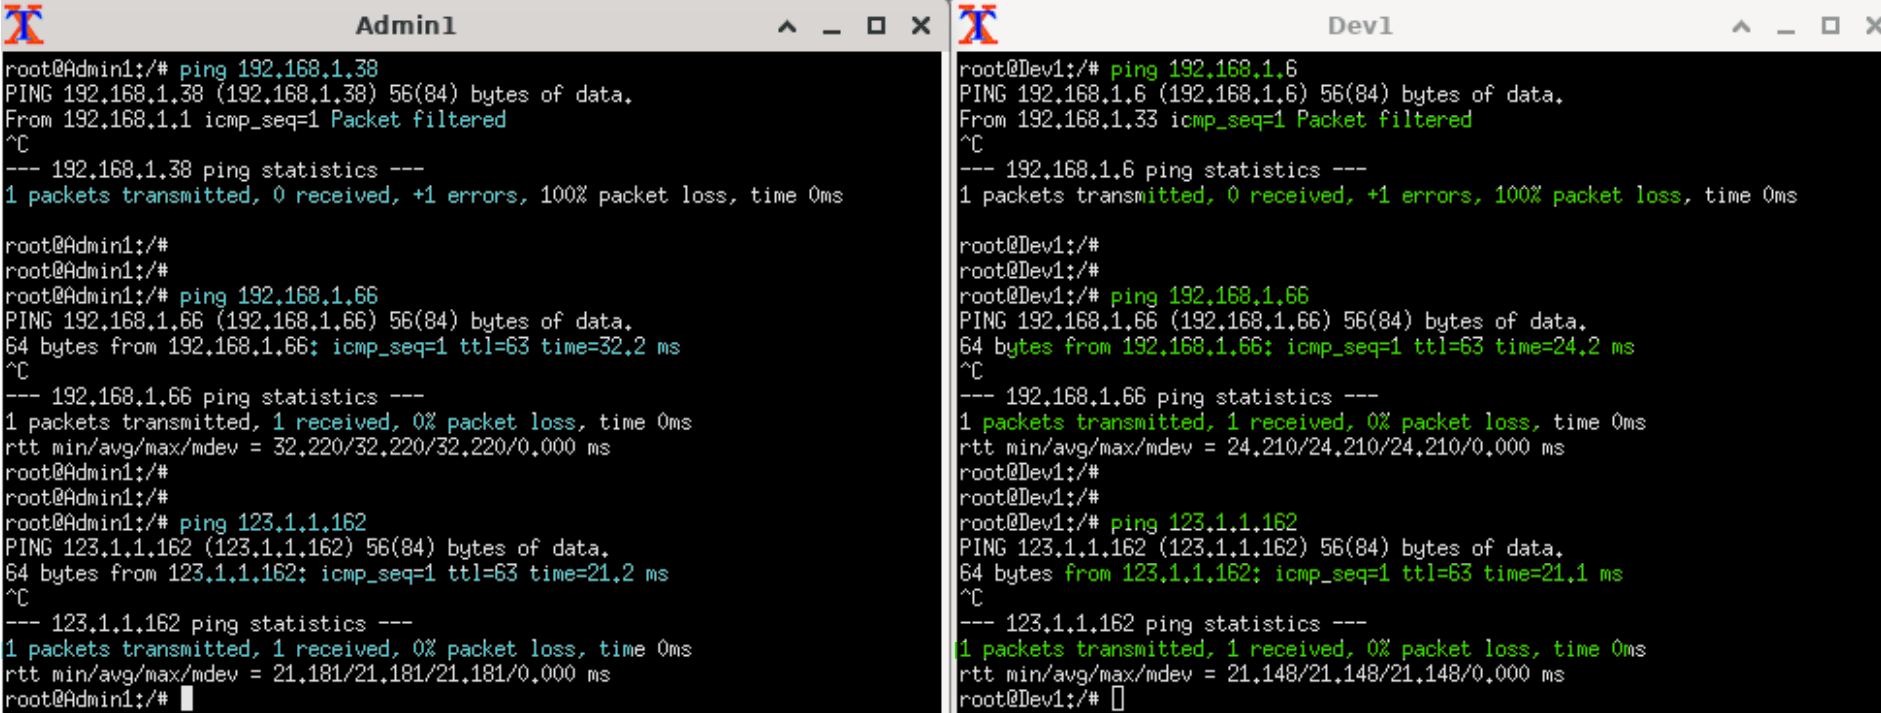
\includegraphics[width=1\textwidth]{../captures/09_ACL_ping_filtre_VLAN1020.png}
	\caption{Tests de connectivité ICMP entre VLAN\_10 et VLAN\_20}
	\label{fig:acl_blocage_vlan10_20}
\end{figure}

La figure~\ref{fig:acl_blocage_vlan31_32} présente des tests similaires entre les VLAN\_31 et VLAN\_32. Les communications entre ces deux réseaux sont également bloquées, tandis que les échanges avec les VLAN utilisateurs restent autorisés.

\begin{figure}[H]
	\centering
	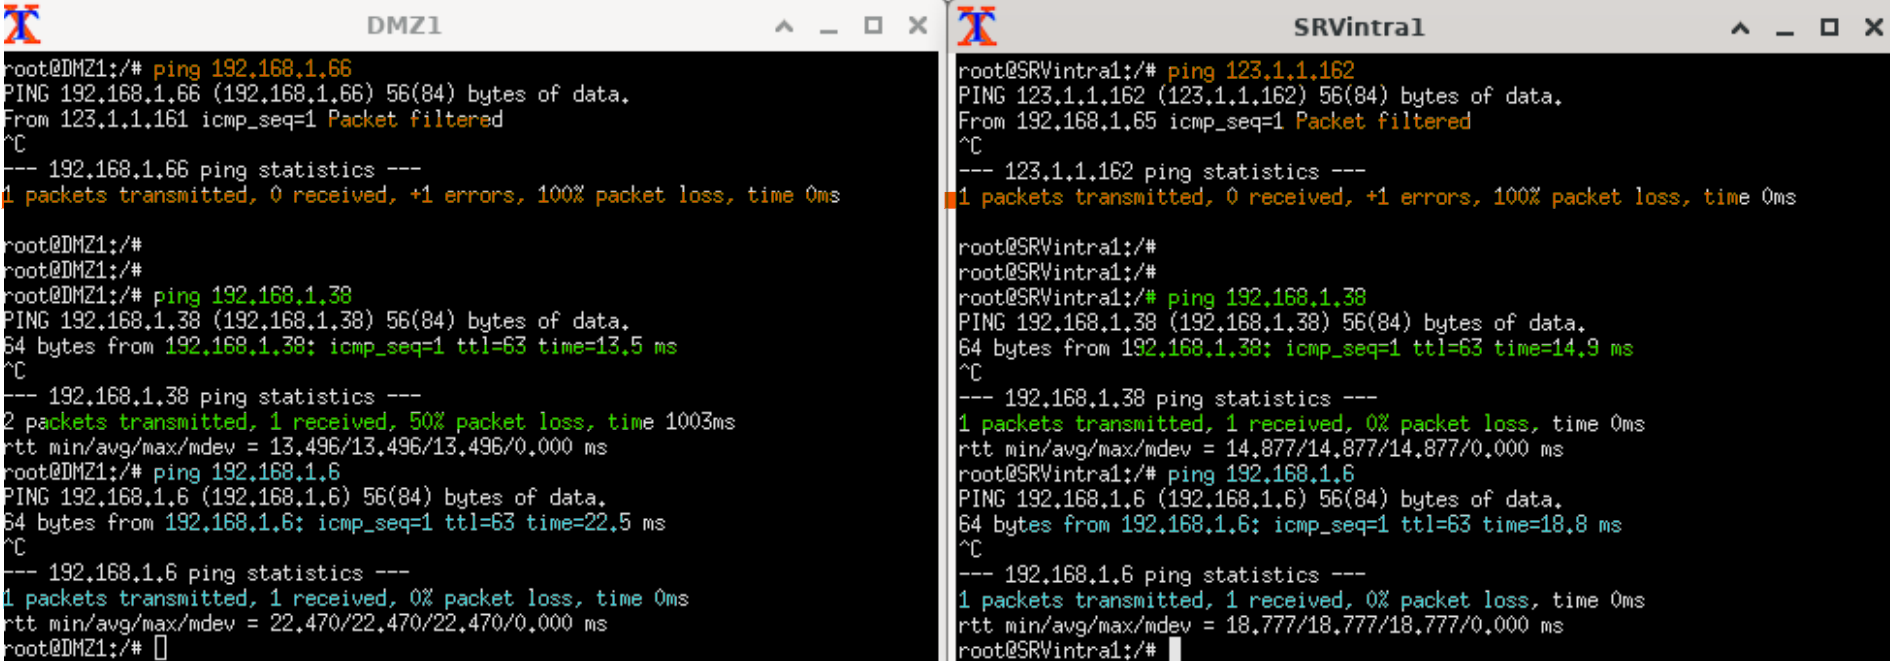
\includegraphics[width=1\textwidth]{../captures/09_ACL_ping_filtre_VLAN3132.png}
	\caption{Tests de connectivité ICMP entre VLAN\_31 et VLAN\_32}
	\label{fig:acl_blocage_vlan31_32}
\end{figure}

La figure~\ref{fig:acl_wireshark} illustre ces comportements à travers des captures de paquets mettant en évidence les flux autorisés et refusés.

\begin{figure}[H]
	\centering
	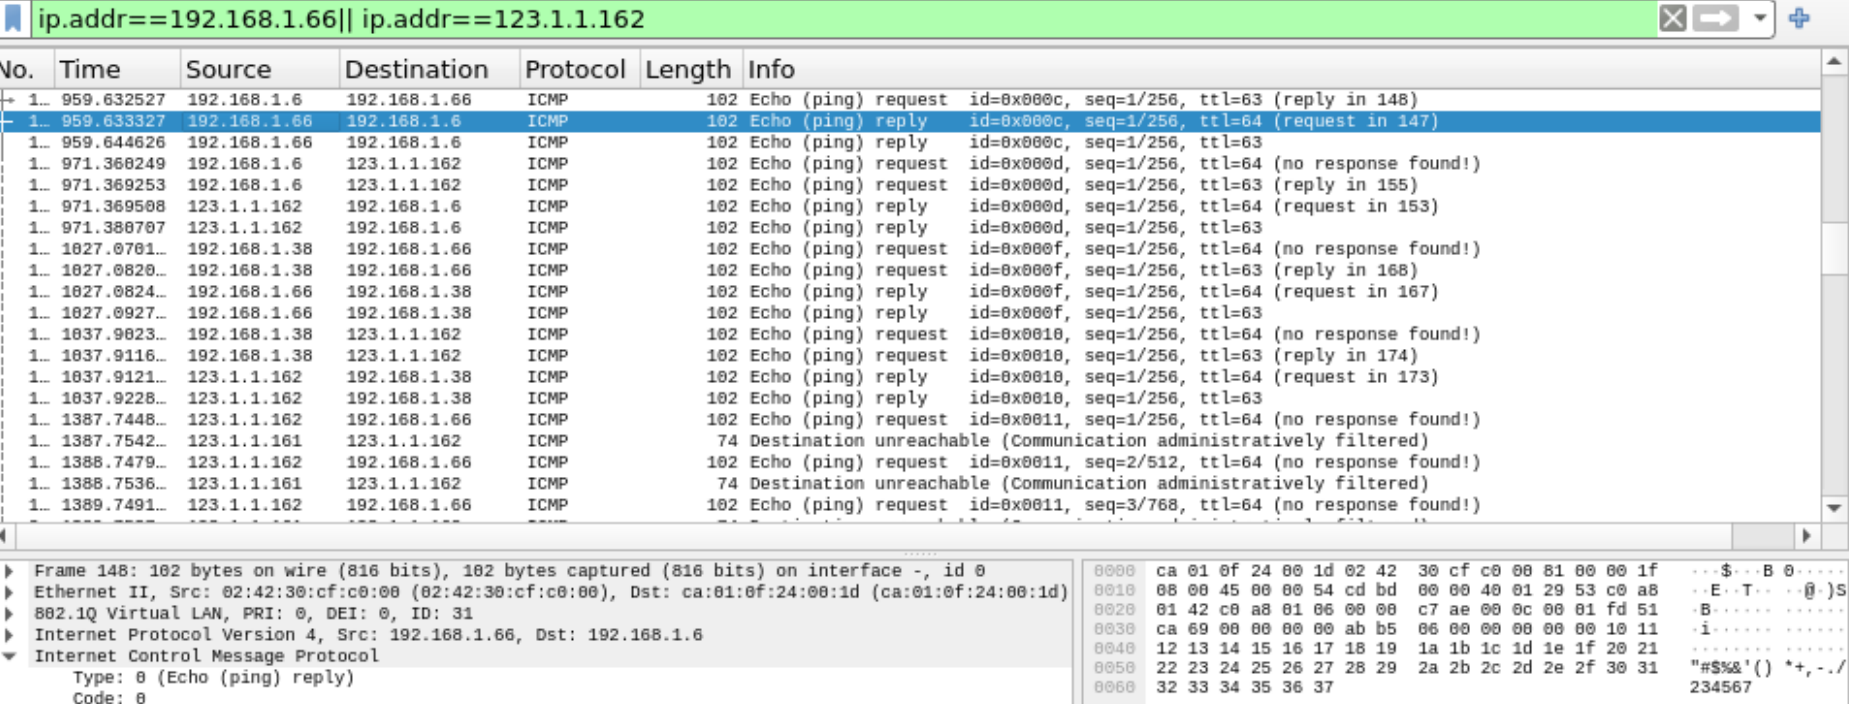
\includegraphics[width=1.1\textwidth]{../captures/09_ACL_wireshark_VLAN3132.png}
	\caption{Analyse Wireshark des flux ICMP (autorisé vs bloqué)}
	\label{fig:acl_wireshark}
\end{figure}
L’analyse des captures réseau réalisées avec Wireshark montre que les paquets ICMP bloqués génèrent un message \textit{"Destination unreachable"} ou \textit{"Packet filtered"}, tandis que les flux autorisés donnent lieu à un échange complet \textit{Echo Request / Echo Reply} avec un taux de réussite de 100\%.

Ces observations confirment que les ACL appliquées filtrent correctement les flux dès leur arrivée sur le routeur, en respectant la politique de sécurité définie. L’isolation des VLANs sensibles est assurée, tout en maintenant les communications nécessaires vers les services internes et externes.

%=================================================
%=================================================
%=================================================

\chapter{Mise en œuvre du réseau opérateur}

\section{Contexte}

La mise en place du réseau opérateur répond à deux objectifs principaux :

\begin{itemize}
	\item disposer d’un réseau IP pleinement opérationnel, reposant sur un routage dynamique au sein du backbone (protocole OSPF), complété par du routage statique entre les routeurs de périphérie et les réseaux clients ;
	
	\item mettre en œuvre des circuits virtuels à l’aide du protocole MPLS, afin d’optimiser l’acheminement des flux et de permettre une isolation logique des trafics.
\end{itemize}

Ainsi, le backbone opérateur repose sur une architecture de type \textbf{IP/MPLS}, dans laquelle le routage IP assure la connectivité globale tandis que MPLS permet une commutation efficace des paquets basée sur des labels.

\section{Présentation de la topologie}

Dans cette seconde partie du projet, l’objectif est de mettre en place un réseau opérateur simulé permettant d’interconnecter les différents sites de l’entreprise ainsi que les infrastructures du fournisseur de cloud (figure~\ref{fig:Topo_op}).

\begin{figure}[H]
	\centering
	\includegraphics[width=0.9\textwidth]{../captures/img3.png}
	\caption{Topologie du réseau opérateur}
	\label{fig:Topo_op}
\end{figure}

Afin de simplifier l’architecture, un unique réseau opérateur est considéré. Celui-ci est structuré autour de deux types de routeurs :

\begin{itemize}
	\item \textbf{Routeurs de cœur (P -- Provider)} : quatre routeurs (RO1 à RO4) interconnectés selon une topologie maillée. Cette organisation permet d’assurer la redondance des chemins et d’améliorer la résilience du réseau en cas de défaillance.
	
	\item \textbf{Routeurs de périphérie (PE -- Provider Edge)} : trois routeurs (RO11, RO21 et RO31) assurant l’interface entre le réseau opérateur et les réseaux externes.
\end{itemize}

Les routeurs de périphérie permettent l’interconnexion avec les différentes entités suivantes :

\begin{itemize}
	\item le réseau du \textbf{Site 1} de l’entreprise via le routeur R1 ;
	\item le réseau du \textbf{Site 2} de l’entreprise via le routeur R2 ;
	\item le réseau \textbf{Intranet} du fournisseur de cloud via le routeur RF1 ;
	\item le réseau \textbf{Public} du fournisseur de cloud via le routeur RF2.
\end{itemize}

Les routeurs RE1, RE2 et RF1 sont considérés comme des routeurs \textbf{CE (Customer Edge)}, situés du côté client et ne participant pas directement au fonctionnement du protocole MPLS.

Chaque interconnexion est réalisée à l’aide de liens d’accès identifiés (A1, A2, B1, B2, C et D), permettant de relier les réseaux externes aux routeurs de périphérie.

Cette architecture met en évidence une séparation claire entre :

\begin{itemize}
	\item le \textbf{cœur de réseau}, chargé du transport des données ;
	\item la \textbf{périphérie}, assurant l’accès aux réseaux clients et aux services.
\end{itemize}

Le choix d’une topologie maillée pour le cœur du réseau constitue un élément clé des infrastructures opérateurs, garantissant la continuité de service grâce à la multiplicité des chemins possibles.

\vspace{0.5cm}
\textbf{Remarque :}

Dans le cadre de cette implémentation, une image spécifique de routeur a été utilisée pour l’ensemble des équipements du réseau opérateur : \texttt{c7200-adventerprisek9-mz.124-24.T5}, importée dans l’environnement GNS3 via le fichier \texttt{cisco-7200-edge.gns3a}.

Cette image permet d’accéder à des fonctionnalités avancées indispensables à la mise en œuvre d’un réseau opérateur, notamment pour le routage dynamique (OSPF) et le support du protocole MPLS.


\section{Plan d’adressage}
Le plan d’adressage du réseau opérateur couvre l’ensemble des liaisons du backbone reliant les routeurs de cœur (RO1 à RO4) ainsi que les routeurs de périphérie (RO11, RO21, RO31).

Pour les interconnexions du backbone, un masque de sous-réseau /30 est retenu, offrant quatre adresses IPv4 par liaison, dont deux utilisables, une pour chaque extrémité.

En ce qui concerne les liaisons point-à-point entre les routeurs de périphérie et les routeurs des clients (sites de l’entreprise et fournisseur cloud), un masque /31 est utilisé. Ce choix permet d’optimiser l’utilisation des adresses IPv4 en supprimant l’adresse de diffusion et en rendant exploitables les deux adresses disponibles sur la liaison.

Le tableau suivant présente le découpage d’adressage retenu pour le backbone et les liaisons d’extrémité du réseau opérateur (hors liens A2 et B2), en indiquant pour chaque liaison :

l’adresse du sous-réseau et le masque associé,

l’adresse de diffusion lorsque applicable,

les adresses attribuées aux ports des routeurs,

et les interfaces correspondantes.
	\begin{center}
		\resizebox{\textwidth}{!}{%
			%		\centering
			%		\caption{Plan d'adressage réseau opérateur}
			%		\renewcommand{\arraystretch}{1.2}
			\begin{tabular}{|l|l|l|l|l|l|}
				\hline
				\textbf{Lien} & \textbf{Sous-réseau /31} & \textbf{IP réseau} & \textbf{IP1 -- IP2} & \textbf{Interfaces} & \textbf{IP boradcast}\\
				\hline
				R1 -- RO11 (A1) & 123.1.1.176/31 & no & 123.1.1.176 -- 123.1.1.177 & f0/0 -- f0/0 & no\\
				R2 -- RO21 (B1) & 123.2.2.168/31 & no & 123.2.2.168 -- 123.2.2.169 & f0/0 -- f0/0 & no\\
				&	&	&	&	&\\		
				RO11 -- RO2 & 12.0.0.0/30 & 12.0.0.0 & 12.0.0.1 -- 12.0.0.2 & e1/0 -- e1/0 & 12.0.0.3\\
				RO21 -- RO3 & 12.0.0.4/30 & 12.0.0.4 & 12.0.0.5 -- 12.0.0.6 & e1/0 -- e1/0 & 12.0.0.7\\
				RO31 -- RO4 & 12.0.0.8/30 & 12.0.0.8 & 12.0.0.9 -- 12.0.0.10 & e1/0 -- e1/0 & 12.0.0.11\\
				&	&	&	&	&\\		
				RO2 -- RO4 & 12.0.0.12/30 & 12.0.0.12 & 12.0.0.13 -- 12.0.0.14 & e1/3 -- e1/3 & 12.0.0.15\\
				RO3 -- RO4 & 12.0.0.16/30 & 12.0.0.16 & 12.0.0.17 -- 12.0.0.18 & e1/1 -- e1/1 & 12.0.0.19\\
				RO2 -- RO1 & 12.0.0.20/30 & 12.0.0.20 & 12.0.0.21 -- 12.0.0.22 & e1/1 -- e1/1 & 12.0.0.23\\
				RO3 -- RO1 & 12.0.0.24/30 & 12.0.0.24 & 12.0.0.25 -- 12.0.O.26 & e1/3 -- e1/3 & 12.0.0.27\\
				RO4 -- RO1 & 12.0.0.28/30 & 12.0.0.28 & 12.0.0.29 -- 12.0.0.30 & e1/2 -- e1/2 & 12.0.0.31\\
				&	&	&	&	&\\		
				RF1 -- RO31 (Intranet) & 163.173.18.254/31 & no & 163.173.18.254 -- 163.173.18.255 & e1/0 -- e1/1 & no \\
				RF2 -- RO31  (Public) & 163.173.19.222/31 & no & 163.173.19.222 --163.173.19.223 & f0/0 -- f0/0 & no\\
				\hline
			\end{tabular}
		}
		%\end{table}
	\end{center}
	
La configuration des interfaces des routeurs s’effectue en mode \textit{configuration terminal}. À titre d’exemple, la configuration de l’interface \texttt{f0/0} du routeur \textbf{R1} est présentée ci-dessous :

\begin{verbatim}
	interface f0/0 
	ip address 123.1.1.176 255.255.255.254 
	no shutdown
\end{verbatim}

Cette procédure est appliquée de manière similaire pour l’ensemble des interfaces des différents routeurs du réseau opérateur.

Le détail complet de la configuration des interfaces pour tous les équipements est fourni dans le document Excel en annexe.
\paragraph{Justification du choix des masques /30 et /31}

Le plan d’adressage du réseau opérateur repose sur l’utilisation de sous-réseaux de petite taille, notamment avec des masques \textbf{/30} et \textbf{/31}, adaptés aux liaisons point-à-point entre routeurs.

\textbf{Utilisation du masque /30}

Le masque \textbf{/30} (255.255.255.252) permet de disposer de 4 adresses IP par sous-réseau :
\begin{itemize}
	\item 1 adresse réseau,
	\item 2 adresses utilisables pour les équipements,
	\item 1 adresse de broadcast.
\end{itemize}

Ce type de masque est historiquement utilisé pour les liaisons point-à-point, car il permet de connecter exactement deux équipements (par exemple deux routeurs) tout en respectant le fonctionnement classique d’IPv4.

\textbf{Utilisation du masque /31}

Le masque \textbf{/31} (255.255.255.254) permet quant à lui de disposer de seulement 2 adresses IP, toutes deux utilisables.

Contrairement aux sous-réseaux classiques, les adresses réseau et broadcast ne sont pas nécessaires dans le cas des liaisons point-à-point. Cette utilisation est définie par la RFC 3021, qui autorise l’emploi du /31 pour ce type de liaison.

Ainsi, le /31 présente plusieurs avantages :
\begin{itemize}
	\item \textbf{Optimisation de l’espace d’adressage IPv4}, en évitant le gaspillage d’adresses ;
	\item \textbf{Adaptation parfaite aux liaisons point-à-point}, qui ne nécessitent que deux adresses ;
	\item \textbf{Réduction de la complexité du plan d’adressage}.
\end{itemize}

\textbf{Choix retenu dans l’architecture}

Dans cette architecture, les deux masques sont utilisés de manière complémentaire :
\begin{itemize}
	\item le \textbf{/31} est privilégié pour les liaisons directes entre routeurs (ex : liaison avec l’opérateur), afin d’optimiser l’utilisation des adresses publiques ;
	\item le \textbf{/30} est utilisé pour les interconnexions internes du réseau opérateur, garantissant une compatibilité maximale avec les équipements et protocoles.
\end{itemize}

Ce choix permet de concilier \textbf{efficacité d’adressage}, \textbf{simplicité de gestion} et \textbf{compatibilité technique}.

%\section{Création d'un réseau opérationnel via les protocoles OSPF et MPLS, LDP}

\section{Mise en œuvre du routage IP}
\subsection{Mise en œuvre du routage IP (OSPF) (routeurs du backbone)}
L’utilisation du routage dynamique, ici avec le protocole \textbf{OSPF} (\textit{Open Shortest Path First}), permet une mise à jour automatique des tables de routage et assure la tolérance aux pannes, ce qui représente un avantage considérable par rapport au routage statique qui nécessite une reconfiguration manuelle en cas de changement de topologie. Par exemple, si le lien RO1–RO2 est défaillant, OSPF recalculera automatiquement un chemin alternatif via RO3 et RO4 sans intervention humaine. 

Le routage dynamique n’est cependant nécessaire que sur les routeurs du backbone de l’opérateur (RO1, RO2, RO3, RO4, RO11, RO21, RO31) afin d’assurer la connectivité interne et la diffusion des routes. Les routeurs clients (R1, R2, RF1, RF2) peuvent se contenter de routes statiques car ils ne possèdent qu’un point d’entrée vers le réseau opérateur.

La configuration du protocole OSPF est réalisée de manière similaire sur l’ensemble des routeurs du backbone, incluant à la fois les routeurs de cœur et les routeurs de périphérie. Tous les routeurs sont intégrés dans une même zone OSPF (area 0), correspondant à l’aire backbone.

À titre d’exemple, la configuration du routage dynamique sur le routeur \textbf{RO1} est présentée ci-dessous :

\begin{verbatim}
	RO1# configure terminal
	RO1(config)# router ospf 1     ! activer le processus OSPF.
	RO1(config-router)# router-id 1.1.1.1    ! identifiant unique du routeur.
	RO1(config-router)# network 12.0.0.20 0.0.0.3 area 0  ! annoncer les sous-
	RO1(config-router)# network 12.0.0.28 0.0.0.3 area 0  ! réseaux directement 
	RO1(config-router)# network 12.0.0.24 0.0.0.3 area 0  ! connectés au routeur
	RO1(config-router)# end                               ! dans l’aire 0.
\end{verbatim}

Le détail complet de la configuration OSPF pour l’ensemble des routeurs est fourni dans le document Excel en annexe.

%-------------------------

\subsection{Routage statique (routeurs clients) et interfaces passives}

Les routeurs clients, à savoir \textbf{R1}, \textbf{R2}, \textbf{RF1} et \textbf{RF2}, ne participent pas au protocole de routage OSPF. En effet, ces équipements n’appartiennent pas au domaine de routage du réseau opérateur.

L’échange de routes entre les routeurs clients et les routeurs de périphérie du réseau opérateur (routeurs PE) est assuré à l’aide de routes statiques. Cette approche permet de simplifier la configuration et de limiter la propagation des informations de routage en dehors du backbone opérateur.

Par conséquent, des routes statiques sont configurées sur ces routeurs afin d’assurer la connectivité avec les réseaux distants.

\medskip

Par ailleurs, afin d’éviter l’établissement de voisinages OSPF avec les routeurs clients, tout en continuant à annoncer leurs réseaux au sein du backbone, les interfaces connectées aux clients (par exemple \texttt{f0/0} sur \textbf{RO11}, \textbf{RO21} et \textbf{RO31}) sont configurées en mode \textit{passive} dans OSPF.

Cette configuration permet :
\begin{itemize}
	\item de \textbf{désactiver l’envoi et la réception des messages OSPF} (Hello) sur ces interfaces ;
	\item de \textbf{prévenir toute tentative de formation d’adjacence OSPF} avec les routeurs clients ;
	\item tout en \textbf{continuant à annoncer les préfixes correspondants} dans le domaine OSPF.
\end{itemize}

Ainsi, les réseaux des sites clients (notamment les adresses IP publiques) restent accessibles depuis l’ensemble du backbone, sans nécessiter l’exécution du protocole OSPF sur les routeurs clients.

\medskip

Un exemple de configuration sur le routeur \textbf{RO11} est donné ci-dessous :

%\textbf{Route statique et interfaces passives sur RO11}
\begin{verbatim}
RO11# configure terminal
	! Route vers le VLAN_32 publique du site 1			
RO11(config)#ip route 123.1.1.160 255.255.255.240 123.1.1.176  
RO11(config)# router ospf 1
	! Redistribuer ces statique le réseau opérateur 		
RO11(config-router)# redistribute static subnets 
	! Définir une interface passive dans l'ospf  
RO11(config-router)# passive-interface f0/0   
RO11(config-router)# network 123.1.1.176 0.0.0.1 area 0
RO11(config-router)# end
\end{verbatim}

 \textbf{ Route par défaut vers l’opérateur}
\begin{verbatim}
	RE1(config)# ip route 0.0.0.0 0.0.0.0 123.1.1.177		
	RE2(config)# ip route 0.0.0.0 0.0.0.0 123.2.2.169		
	RF2(config)# ip route 0.0.0.0 0.0.0.0 163.173.19.223			
\end{verbatim}

\subsection{Validation du fonctionnement du protocole OSPF}

Afin de vérifier le bon fonctionnement du protocole de routage dynamique OSPF au sein du réseau opérateur, une analyse du trafic ainsi que des états de voisinage a été réalisée.


\subsubsection{Wiresharque (Hello \& LS Update \& voisinage)}
L’observation des captures réseau met en évidence la présence de messages OSPF de type \textit{Hello}, échangés périodiquement entre les routeurs adjacents (fig.~\ref{fig:ospf_lsupdate}). Ces messages permettent :
\begin{itemize}
	\item la découverte des routeurs voisins ;
	\item le maintien des relations de voisinage ;
	\item la détection d’éventuelles pertes de connectivité.
\end{itemize}

\begin{figure}[H]
	\centering
	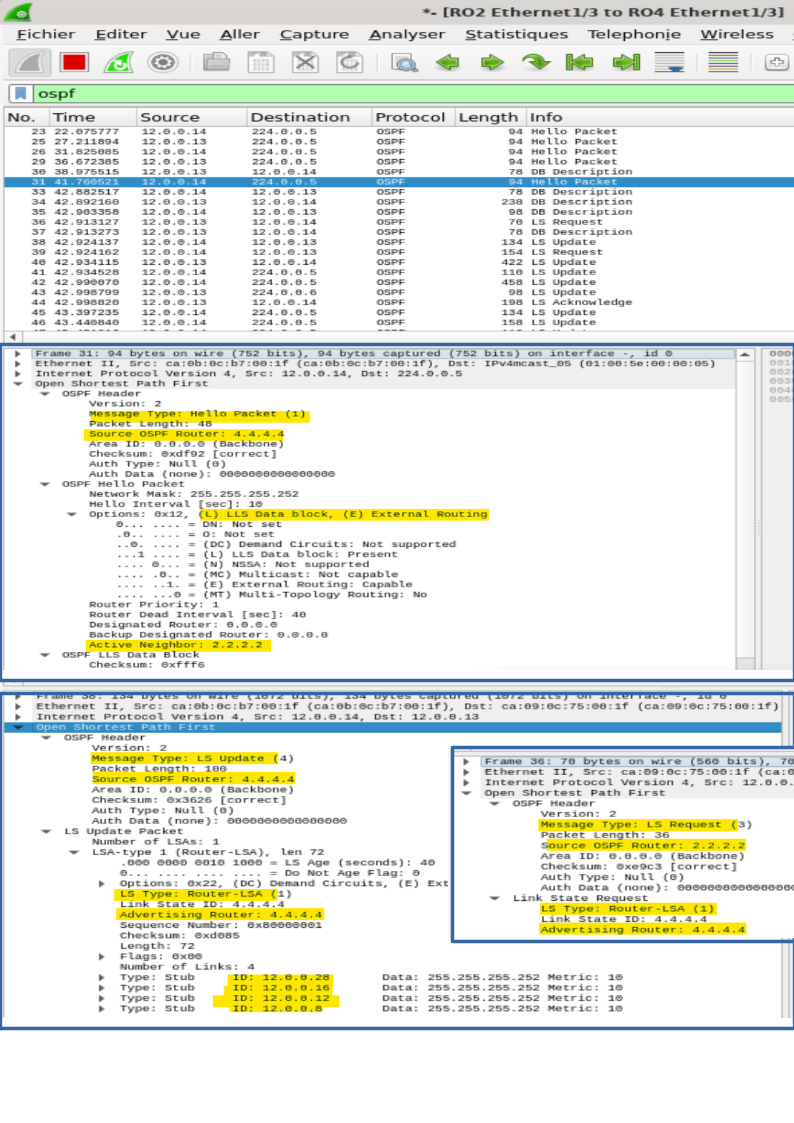
\includegraphics[width=0.81\textwidth]{../captures/10_ospf_lsupdate.png}
	\caption{Capture Wireshark des échanges OSPF après modification de topologie : observation des messages Hello et des paquets LS Update diffusant les informations de routage}
	\label{fig:ospf_lsupdate}
\end{figure}

Par ailleurs, la formation des adjacences OSPF a été vérifiée à l’aide des commandes de diagnostic (par exemple \texttt{show ip ospf neighbor}), confirmant que les routeurs du backbone ont bien établi des relations de voisinage complètes.
\begin{figure}[H]
	\centering
	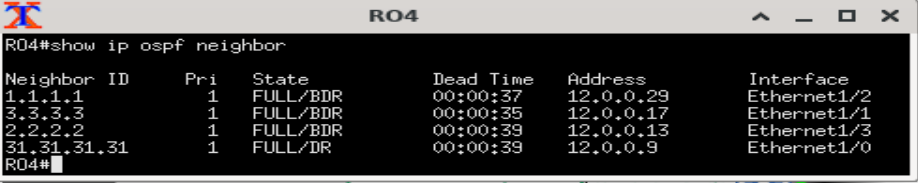
\includegraphics[width=0.8\textwidth]{../captures/10_ospf_neighbors.png}
	\caption{Table des voisins OSPF sur le routeur RO4 : adjacences établies avec les routeurs du backbone (état \textit{FULL})}
	\label{fig:ospf_neighbors_ro4}
\end{figure}
Une fois ces adjacences établies, les routeurs échangent leur base de données de topologie, permettant la construction d’une vision cohérente du réseau. 

\textbf{Remarque : \\} L’absence de messages de type \textit{LS Update} dans les captures s’explique par le fait que le réseau est dans un état stable, sans modification de topologie. 

Pour visualiser un \textit{LS Update}, on peut le provoquer ainsi : 
\begin{verbatim}
	RO11(config)#shutdown interface e1/0
	RO11(config)#no shutdown
\end{verbatim}

\subsubsection{Tests de la connectivité du réseau opérateur}
Enfin, pour valider le bon fonctionnement du routage dynamique OSPF au sein du réseau opérateur, des tests de connectivité peuvent être réaliser entre différents équipements dans les situations suivantes :
\begin{enumerate}
	\item  entre toutes paires de routeurs des réseaux extrémités : R1, R2 et RF2,
	\item entre chaque sous-réseau privé du Site x vers un serveur accessible par Internet du Site y,
	\item entre chaque sous-réseau privé ou public du Site x de l’entreprise et le routeur RF2,
	\item entre chaque sous-réseau privé du Site x vers un serveur accessible par Internet hébergé chez le Fournisseur de Cloud.
\end{enumerate}



\textbf{Exemple de tests de connectivité entre les routeurs clients \textbf{R1}, \textbf{R2} et le réseau distant \textbf{RF2}}\\
La figure~\ref{fig:connectivite_operateur} présente des tests de connectivité réalisés depuis les routeurs \textbf{R1} et \textbf{R2}, incluant des commandes \texttt{ping} et \texttt{traceroute} vers différents réseaux distants.

\begin{figure}[H]
	\centering
	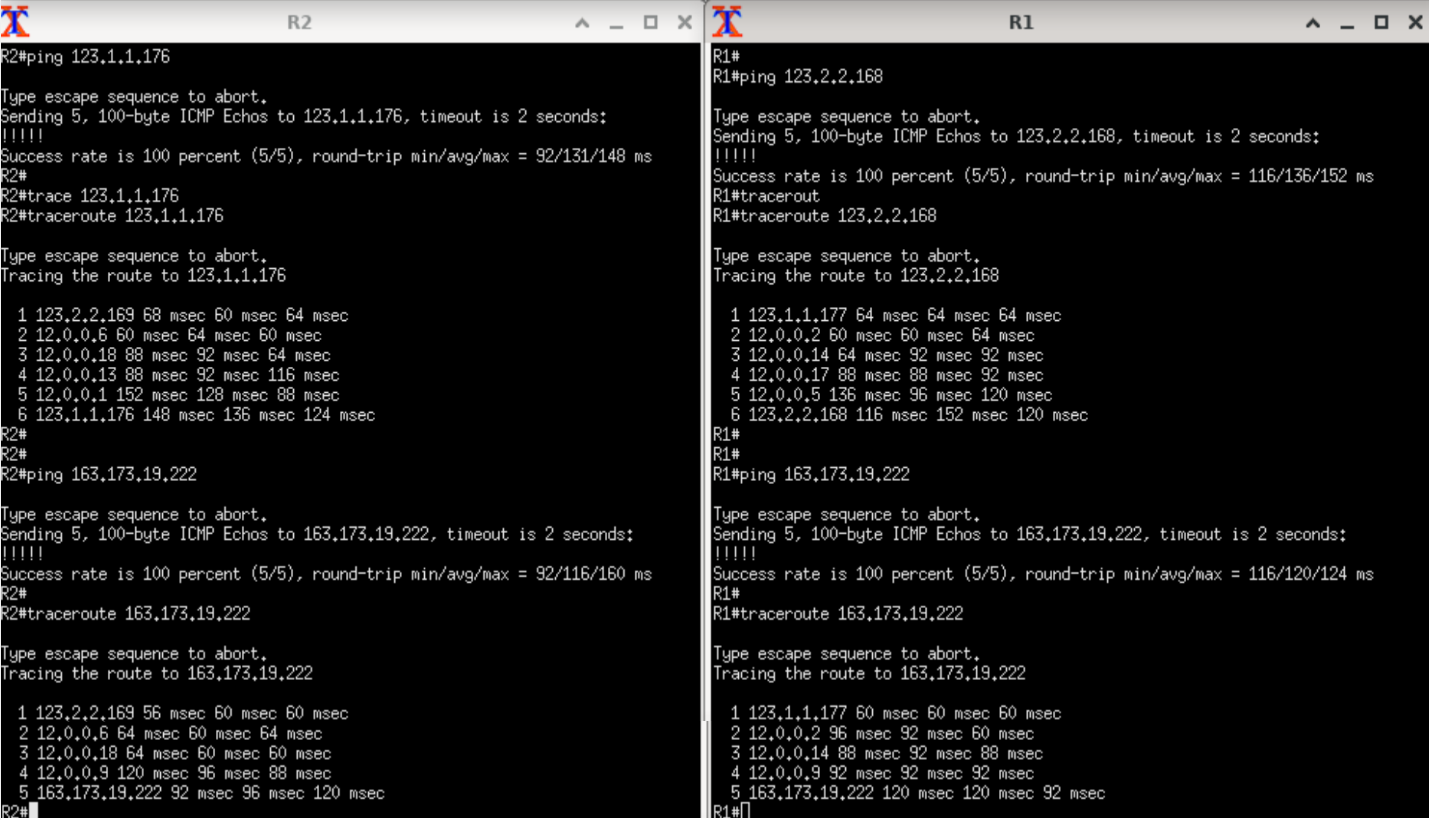
\includegraphics[width=\textwidth]{../captures/10_ospf_connexion_routeurs.png}
	\caption{Tests de connectivité depuis R1 et R2 : validation du routage avec \texttt{ping} (100\% de réussite) et visualisation des chemins avec \texttt{traceroute} à travers le backbone opérateur}
	\label{fig:connectivite_operateur}
\end{figure}



\begin{enumerate}
	\item \textbf{Tests ICMP (ping)} : 
	
	Les tests de type ICMP (\texttt{ping}) montrent un taux de réussite de \textbf{100\%} entre les différents points testés :
	
	\begin{itemize}
		\item Depuis \textbf{R2} vers \texttt{123.1.1.176} (site 1)
		\item Depuis \textbf{R1} vers \texttt{123.2.2.168} (site 2)
		\item Depuis \textbf{R1} et \textbf{R2} vers \texttt{163.173.19.222} (réseau distant)
	\end{itemize}
	
	Ces résultats confirment que :
	\begin{itemize}
		\item les routes sont correctement propagées via OSPF dans le backbone ;
		\item les routes statiques côté clients sont correctement configurées ;
		\item la connectivité inter-sites et vers les réseaux externes est fonctionnelle.
	\end{itemize}
	
	\item \textbf{Analyse des chemins (traceroute)}
	
	Les commandes \texttt{traceroute} permettent d’observer le chemin emprunté par les paquets à travers le réseau opérateur.
	
	Les résultats montrent que :
	\begin{itemize}
		\item les paquets traversent successivement les routeurs de périphérie (RO11, RO21) puis les routeurs du cœur (RO1 à RO4) ;
		\item plusieurs sauts intermédiaires correspondent aux adresses du réseau backbone (\texttt{12.0.0.x}) ;
		\item le chemin est cohérent avec la topologie maillée du réseau opérateur.
	\end{itemize}
	
	Cela confirme que :
	\begin{itemize}
		\item le protocole OSPF calcule correctement les routes ;
		\item les chemins sélectionnés respectent la connectivité du backbone ;
		\item la convergence du réseau est effective.
	\end{itemize}
	
	\item \textbf{Observation du trafic réseau}
	
	Une capture de trafic réalisée entre les routeurs \textbf{RO11} et \textbf{RO2} met en évidence la circulation des paquets ICMP ainsi que les échanges liés au protocole OSPF.
	
	\begin{figure}[H]
		\centering
		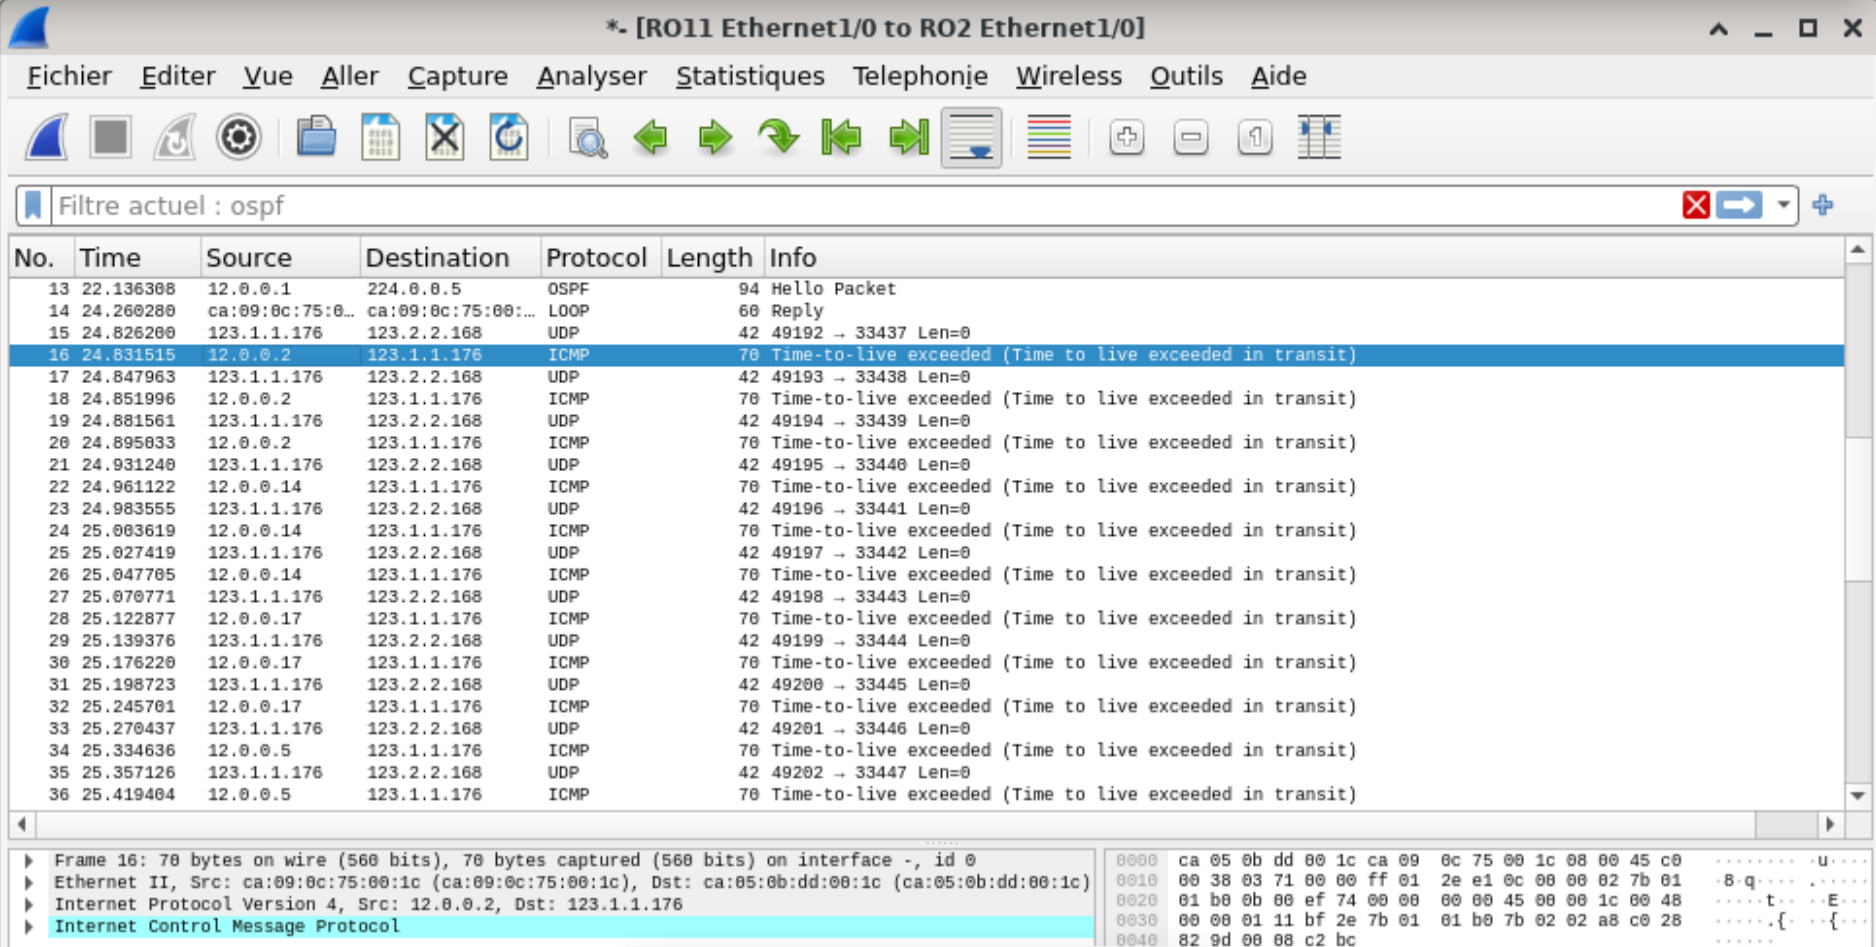
\includegraphics[width=\textwidth]{../captures/10_ospf_connexion_routeurs_wireshark.png}
		\caption{Capture de trafic entre RO11 et RO2 : observation des échanges ICMP et OSPF}
		\label{fig:wireshark_operateur}
	\end{figure}
	
	L’analyse de cette capture montre les éléments suivants :
	\begin{itemize}
		\item le passage des requêtes ICMP (Echo Request) et des réponses (Echo Reply) entre les routeurs ;
		\item la présence de paquets OSPF (Hello, LS Update), confirmant l’établissement des voisinages ;
		\item une transmission correcte des paquets sans perte ni anomalie.
	\end{itemize}

%\end{enumerate}
	
%\subsubsection{Validation de la diffusion des routes externes}
	\item \textbf{{Validation de la diffusion des routes externes}}
	
Afin de vérifier la propagation des routes externes dans le domaine OSPF, la commande suivante a été utilisée sur les routeurs de périphérie RO11, RO21 et RO31:

\begin{verbatim}
	RO11# show ip ospf database external
\end{verbatim}

La commande \texttt{show ip ospf database external} permet de visualiser les routes externes injectées dans le processus OSPF. Ces routes correspondent à des réseaux non appris nativement via OSPF, mais introduits par redistribution ou via des routes statiques.

Les entrées observées dans cette base correspondent à des \textbf{LSA de type 5} (\textit{External LSA}), identifiées par leur préfixe réseau et le routeur annonceur (ASBR). Chaque LSA contient notamment :
\begin{itemize}
	\item le réseau de destination ;
	\item la métrique associée ;
	\item le type de métrique (1 ou 2) ;
	\item l’identifiant du routeur ayant injecté la route.
\end{itemize}

La présence de ces LSA sur l’ensemble des routeurs analysés confirme que les routes externes sont correctement propagées dans le backbone OSPF. Cela permet aux routeurs internes d’avoir une visibilité complète des réseaux situés en dehors du domaine OSPF, notamment les réseaux publics et les infrastructures du fournisseur de cloud.

\paragraph{Observations sur les routeurs}

La figure~\ref{fig:ospf_ext_example} illustre un exemple de routes externes (LSA de type 5) observées sur un routeur du backbone (RO11).

Des résultats similaires ont été obtenus sur les routeurs RO21 et RO31, confirmant que les routes externes sont correctement propagées à l’ensemble du domaine OSPF.

Cette cohérence entre les différents équipements valide le bon fonctionnement de la diffusion des routes externes dans le réseau opérateur.

\textbf{Routeur RO11}

\begin{figure}[H]
	\centering
	\includegraphics[width=0.9\textwidth]{../captures/11_ospf_database_external.png}
	\caption{Exemple de LSA externes (type 5) observés sur un routeur du backbone}
	\label{fig:ospf_ext_example}
\end{figure}

\end{enumerate}
Les observations sont identiques sur l’ensemble des routeurs du backbone, ce qui confirme la cohérence de la base de données OSPF (LSDB).


\textbf{Conclusion :}

Les tests de connectivité (ping et traceroute ainsi le database external) confirment que les routes calculées par OSPF sont correctement utilisées pour acheminer les paquets à travers le réseau opérateur.

Ainsi, l’ensemble de ces observations (messages Hello, formation des adjacences, stabilité du réseau et connectivité effective) permet de valider le bon fonctionnement du protocole OSPF dans l’architecture mise en place.

\subsection{Mise en œuvre du protocole MPLS}
\subsubsection{Activation de MPLS et du protocole LDP}

Sur l’ensemble des routeurs du réseau opérateur (RO1 à RO4, RO11, RO21, RO31), le mécanisme CEF (\textit{Cisco Express Forwarding}) est activé. Cette fonctionnalité est indispensable au bon fonctionnement de MPLS, car elle permet une commutation rapide des paquets basée sur des tables de transfert optimisées.

Le protocole MPLS ainsi que le protocole de distribution de labels LDP (\textit{Label Distribution Protocol}) sont ensuite activés uniquement sur les interfaces du backbone du réseau opérateur.

En revanche, aucune configuration MPLS/LDP n’est appliquée sur les liaisons d’accès reliant les routeurs clients (R1, R2) aux routeurs de périphérie (RO11, RO21). Ces interfaces restent en routage IP classique, conformément au modèle CE/PE, où seuls les routeurs du cœur et de périphérie participent au transport MPLS.

Un exemple de configuration est présenté ci-dessous, le détail complet étant fourni en annexe dans le fichier Excel.

\begin{verbatim}
	! Activer CEF (obligatoire pour MPLS)
	RO11(config)# ip cef
	
	! Activer MPLS globalement
	RO11(config)# mpls ip
	
	! Définir le protocole de distribution de labels (LDP)
	RO11(config)# mpls label protocol ldp
	
	! Activer MPLS sur une interface du backbone
	RO11(config)# interface e1/0
	RO11(config-if)# mpls ip
\end{verbatim}

Ainsi, les routeurs PE assurent l’insertion et la suppression des labels MPLS, tandis que les routeurs P réalisent uniquement la commutation basée sur ces labels.

\subsubsection{Vérification des voisins LDP}

La commande \texttt{show mpls ldp neighbor} permet de vérifier l’établissement des sessions LDP entre les routeurs du backbone.

Les résultats obtenus montrent que chaque routeur MPLS établit correctement des relations de voisinage avec ses routeurs adjacents. Ces échanges permettent la distribution des labels nécessaires à la mise en place des chemins MPLS.

La présence de voisins LDP actifs confirme que le plan de contrôle MPLS est opérationnel (fig.~\ref{fig:mpls_example}).
\begin{figure}[H]
	\centering
	\includegraphics[width=0.9\textwidth]{../captures/12_mpls_results.png}
	\caption{Exemple d'établissement des sessions LDP entre le routeur RO11 et le reste des routeurs de backbone}
	\label{fig:mpls_example}
\end{figure}
\subsubsection{Analyse de la table de commutation MPLS}

La commande \texttt{show mpls forwarding-table} permet de visualiser les labels associés aux différents préfixes réseau.

Cette table indique (fig.~\ref{fig:mpls_example}), pour chaque destination :
\begin{itemize}
	\item le label local attribué ;
	\item le label de sortie ;
	\item l’interface de sortie ;
	\item le prochain saut.
\end{itemize}

L’analyse de cette table met en évidence que les paquets ne sont plus routés uniquement sur la base de l’adresse IP, mais commutés en fonction des labels MPLS.

Cela confirme le bon fonctionnement du plan de données MPLS.

\subsubsection{Tests de connectivité}

Des tests de connectivité ont été réalisés à l’aide des commandes \texttt{ping} et \texttt{traceroute} entre les différents routeurs et réseaux (fig.~\ref{fig:mpls_ping}).

\begin{figure}[H]
	\centering
	\includegraphics[width=0.9\textwidth]{../captures/12_mpls_ping_RO11.png}
	\caption{Exemple de test de connectivité entre les routeurs RO11 et R2}
	\label{fig:mpls_ping}
\end{figure}

Les résultats montrent que les communications sont correctement établies à travers le backbone MPLS. Les chemins empruntés sont cohérents avec la topologie du réseau.

Ces tests confirment que MPLS fonctionne correctement et assure le transport des paquets entre les différents sites.


\subsubsection{Perte d'adjacence}
Si un routeur du backbone tombe, OSPF détecte la perte d’adjacence, reconstruit la topologie et recalculera les routes (ré-installation des routes et ré-distribution de labels MPLS) (fig.~\ref{ospf_panne1}). Pendant la reconvergence on observera pertes/transitoires, TTL expired dans traceroute ou hop manquant ; une fois OSPF/MPLS reconvergés, le trafic emprunte le chemin alterné disponible.
Techniquement voici les étapes de ce qui se passe :
\begin{itemize}
	\item Lien ou routeur tombe → adjacences OSPF se brisent
	\item Les voisins détectent la disparition (Hello timeouts).
	\item show ip ospf neighbor passe du statut FULL à DOWN/INIT/2-way.
	\item OSPF reconstruit la LSDB et recalcule SPF
	\item Chaque routeur recalcule les routes (nouvelle RIB).
	\item Les routes affectées peuvent être supprimées ou changées de next-hop.
	\item MPLS/LDP : mise à jour des labels
	\item LDP détecte la perte de session LDP avec le voisin → les labels associés sont supprimés.
	\item Les routeurs recalculent LFIB (forwarding-table). Si un chemin alternatif via d’autres PE/P est disponible, de nouveaux labels sont assignés et distribués.
	\item Conséquences visibles côté utilisateur
	ping échoue temporairement, traceroute montre TTL exceeded / * / sauts changeants / alternance
	Possibles paquets perdus ou sessions TCP reset avant que la nouvelle route soit utilisée.
\end{itemize}


\begin{figure}[H]
	\centering
	\includegraphics[width=\textwidth]{../captures/12_mpls_ping_RO11.png}
	\caption{Disparition des routes utilisées par RO11 ou changement de next-hop}
	\label{ospf_panne1}
\end{figure}

\subsubsection{Joignabilité des réseaux privés depuis l'extérieur}
 Les paquets arrivant depuis RF1/RF2 ne pourront pas atteindre les hôtes privés ou les réponses ne reviendront pas. 
 
 Dans notre topologie, les hôtes privés (192.168.x.x) sortent vers Internet en étant traduits (NAT) sur R1/R2.
 
 Par défaut, NAT overload (ip nat inside source list X interface FastEthernet0/0 overload) n’accepte pas les connexions entrantes non sollicitées : il traduit les flux sortants mais ne mappe pas une connexion entrante vers un hôte interne

Donc un ping/connexion initiée depuis RF1 ou RF2 vers une IP privée des deux sites ne peut pas traverser R1 ni R2 pour atteindre l’hôte privé, à moins qu'on fasse de la redirection (fig.~\ref{ospf_RF1-prive}).

\begin{figure}[H]
	\centering
	\includegraphics[width=\textwidth]{../captures/13_connectivite_RF1_prive.png}
	\caption{Injoignabilité des réseaux privés depuis le routeur RF1}
	\label{ospf_RF1-prive}
\end{figure}


\chapter{Tunnel d'interconnexion}
\section{Objectif}
Cette troisième partie du projet a pour objectif d’étendre les capacités du réseau opérateur en mettant en place des mécanismes d’interconnexion avancés entre les différents sites de l’entreprise et les infrastructures du fournisseur de cloud. Dans un premier temps, un tunnel de type \textbf{L2VPN basé sur MPLS} est déployé afin d’assurer une continuité des réseaux locaux entre les Sites 1 et 2. Ce mécanisme permet de transporter les trames Ethernet de manière transparente à travers le backbone opérateur, offrant ainsi l’illusion d’un réseau local unique, tout en conservant l’encapsulation VLAN existante. Dans un second temps, un tunnel de type \textbf{L3VPN basé sur GRE} est mis en œuvre pour interconnecter les sous-réseaux applicatifs avec le réseau Intranet du fournisseur de cloud. Contrairement au L2VPN, ce tunnel fonctionne au niveau IP et permet l’échange de datagrammes entre des réseaux distincts. L’objectif global est donc de combiner ces deux approches afin d’assurer à la fois une extension des réseaux locaux entre sites et une interconnexion sécurisée et structurée avec les services externes, tout en s’appuyant sur l’infrastructure IP/MPLS mise en place précédemment.

%----------------------------------------------
\section{Interconnexion des sites via MPLS (L2VPN)}

\subsection{Schéma Général des Tunnel L2VPN}
\begin{figure}[H]
	\centering
	\begin{tikzpicture}[>=latex, node distance=3cm, every node/.style={draw, rounded corners, minimum width=2.5cm, minimum height=1cm, align=center}]
		
		% Sites
		\node (R1) {R1 \\ Site 1};
		\node (R2) [right=5cm of R1] {R2 \\ Site 2};
		%		\node (RE2) [right=8cm of RE1] {RE2 \\ Site 2};
		
		% Opérateur
		\node (RO11) [above=3cm of R1] {RO11 \\ Opérateur};
		\node (RO21) [above=3cm of R2] {RO21 \\ Opérateur};
		
		% Liaisons CE->PE
		\draw[->, thick] (R1) -- node[left] {e1/2.10, e1/2.20, e1/2.31} (RO11);
		\draw[->, thick] (R2) -- node[right] {e1/2.10, e1/2.20, e1/2.31} (RO21);
		
		% Tunnel MPLS
		\draw[<->, dashed, thick, red] (RO11) -- (RO21);
		
		% Texte sur le tunnel
		\node[draw=none, above=0.4cm] at ($(RO11)!0.5!(RO21)$) {MPLS: LSP label + VPN label};
		\node[draw=none, below=0.2cm] at ($(RO11)!0.5!(RO21)$) {Tunnel L2VPN MPLS};
		
		
		% VLANs LAN_x-1, LAN_x-2, LAN_x-31
		\node[draw, below=1cm of R1] (LAN1) {LAN\_1-1, LAN\_1-2, LAN\_1-31};
		\node[draw, below=1cm of R2] (LAN2) {LAN\_2-1, LAN\_2-2, LAN\_2-31};
		
		\draw[->, thick] (LAN1.north) -- (R1.south);
		\draw[->, thick] (LAN2.north) -- (R2.south);
		
	\end{tikzpicture}
	\caption{Schéma logique MPLS L2VPN pour l’interconnexion des sites de l’entreprise}
\end{figure}
\begin{itemize}
	\item Les routeurs d’extrémité client (Customer Edge – CE), R1 et R2 se connectent respectivement aux VLAN_10, VLAN_20 et VLAN_31. 
	
	\item Les routeurs opérateurs (Provider Edge – PE), RO11 et RO21,  leur rôle est de terminer les sessions MPLS et de créer les tunnels L2VPN VPWS (Virtual Private Wire Service). Ils sont reliés aux CE (R1 et R2) via des sous-interfaces Ethernet (interface physique e1/2) taguées (VLAN 10, 20, 31).
	
	\item La liaisons R1 → RO11 (R2 → RO21) est représentée par une flèche où chaque sous-interface, e1/2.10, e1/2.20 ou e1/2.31, transporte le trafic de son VLAN spécifique.
	
	Ce trafic est encapsulé par les PE (RO11/RO21) via le protocole MPLS.
	
	\item Tunnel MPLS entre RO11 et RO21, représenté par une liaison pointillée ({\color{red}<$\dot{---}$>}). Le texte associé précise la double hiérarchie d’étiquettes MPLS :\\
	LSP label : utilisé pour acheminer les paquets dans le cœur MPLS.\\
	VPN label : utilisé pour identifier le pseudowire correspondant à un VLAN (10, 20, 31).
	
	C’est ce mécanisme qui permet d’offrir un service L2VPN (VPWS).
	
	\item Les blocs (LAN_1-1, LAN_1-2, LAN_1-31) et (LAN_2-1, LAN_2-2, LAN_2-3), représentent les réseaux locaux des deux sites. Chaque VLAN (10, 20, 31) correspond à un sous-réseau spécifique. Grâce au tunnel MPLS, les VLANs sont étendus d’un site à l’autre comme si les deux LANs étaient sur le même switch étendu.
\end{itemize}

Avec cette configuration, chaque VLAN des sites 1 et 2 est prolongé sur le tunnel L2VPN MPLS. Les employés de VLAN identiques sur les deux sites peuvent communiquer comme s’ils étaient sur le même LAN.

\subsection{Plan d'adressage}
	\begin{center}
		\resizebox{\textwidth}{!}{%
			%	\caption{Tableau d’adressage pour la première évolution (Tunnel L2VPN MPLS)}
			\begin{tabular}{|c|c|c|c|c|c|c|c|}
				\hline
				Site & VLAN & Sous-réseau & Interface CE/RE & IP RE & IP PE & Masque & Tunnel MPLS ID \\
				\hline
				1 & 10 & LAN\_1-1 &  R1 e1/2.10 & 192.168.0.0 & -- & /31 & 101 \\
				& 20 & LAN\_1-2 & R1 e1/2.20 & 192.168.0.2 & -- & /31 & 101 \\
				& 31 & LAN\_1-31 & R1 e1/2.31 & 192.168.0.4 & -- & /31 & 101 \\
				\hline		
				2 & 10 & LAN\_2-1 & R2 e1/2.10 & 192.168.0.1 & -- & /31 & 101 \\
				& 20 & LAN\_2-2 & R2 e1/2.20 & 192.168.0.3 & -- & /31 & 101 \\
				& 31 & LAN\_2-31 & R2 e1/2.31 & 192.168.0.5 & -- & /31 & 101 \\
				\hline
				RO11 &-- & Loopback PE & Loopback0 & -- & 192.168.0.11 & /32 & -- \\
				RO21 &-- & Loopback PE & Loopback0 & -- & 192.168.0.21 & /32 & -- \\
				\hline
			\end{tabular}
		}
	\end{center}

	\subsection{Implémentations nécessaires sur les routeurs clients }
	Le schéma ci-dessous représente le flue des trames à travers le tunnel L2VPN via le protocole MPLS où on ne voit que les routeurs (CE) R1 et R2.
	
	\vline 
	
	\begin{tikzpicture}[node distance=6.5cm, thick, >=latex]
		%	xshift=-3cm
		% Style des boîtes
		\tikzstyle{router}=[draw, rounded corners=2pt, minimum width=1.5cm, minimum height=3.5cm, align=center]
		
		% Les deux box
		\node[router] (R1) {R1};
		\node[router, right=4.5cm of R1] (R2) {R2};
		
		%--- Définition des "ports" (coordonnées) ---
		% RE1 : ports LAN (gauche)
		\path (R1.west) ++(0, 1.0) coordinate (R1L10);
		\path (R1.west) ++(0, 0.0) coordinate (R1L20);
		\path (R1.west) ++(0,-1.0) coordinate (R1L31);
		
		% R1 : ports inter-site (droite)
		\path (R1.east) ++(0, 1.0) coordinate (R1X10);
		\path (R1.east) ++(0, 0.0) coordinate (R1X20);
		\path (R1.east) ++(0,-1.0) coordinate (R1X31);
		
		% R2 : ports inter-site (gauche)
		\path (R2.west) ++(0, 1.0) coordinate (R2X10);
		\path (R2.west) ++(0, 0.0) coordinate (R2X20);
		\path (R2.west) ++(0,-1.0) coordinate (R2X31);
		
		% R2 : ports LAN (droite)
		\path (R2.east) ++(0, 1.0) coordinate (R2R10);
		\path (R2.east) ++(0, 0.0) coordinate (R2R20);
		\path (R2.east) ++(0,-1.0) coordinate (R2R31);
		
		%--- Dessin des petits carrés (ports visuels) ---
		% Ports R1 côté gauche (vers l'extérieur à gauche)
		\filldraw[fill=white] (R1L10) ++(-0.18, 0.12) rectangle ++(0.18,-0.24);
		\filldraw[fill=white] (R1L20) ++(-0.18, 0.12) rectangle ++(0.18,-0.24);
		\filldraw[fill=white] (R1L31) ++(-0.18, 0.12) rectangle ++(0.18,-0.24);
		
		% Ports R1 côté droit (vers l'extérieur à droite)
		\filldraw[fill=white] (R1X10) ++( 0.00, 0.12) rectangle ++(0.18,-0.24);
		\filldraw[fill=white] (R1X20) ++( 0.00, 0.12) rectangle ++(0.18,-0.24);
		\filldraw[fill=white] (R1X31) ++( 0.00, 0.12) rectangle ++(0.18,-0.24);
		
		% Ports R2 côté gauche (vers l'extérieur à gauche)
		\filldraw[fill=white] (R2X10) ++(-0.18, 0.12) rectangle ++(0.18,-0.24);
		\filldraw[fill=white] (R2X20) ++(-0.18, 0.12) rectangle ++(0.18,-0.24);
		\filldraw[fill=white] (R2X31) ++(-0.18, 0.12) rectangle ++(0.18,-0.24);
		
		% Ports R2 côté droit (vers l'extérieur à droite)
		\filldraw[fill=white] (R2R10) ++( 0.00, 0.12) rectangle ++(0.18,-0.24);
		\filldraw[fill=white] (R2R20) ++( 0.00, 0.12) rectangle ++(0.18,-0.24);
		\filldraw[fill=white] (R2R31) ++( 0.00, 0.12) rectangle ++(0.18,-0.24);
		
		%--- Liaisons LAN vers R1 (gauche) ---
		\draw (R1L10) ++(-0.20,0) -- ++(-2.2,0) node[left, above]{192.168.1.0/27 :\color{blue}e1/1.10};
		\draw (R1L20) ++(-0.20,0) -- ++(-2.2,0) node[left, above]{192.168.1.32/27 :\color{blue}e1/1.20};
		\draw (R1L31) ++(-0.20,0) -- ++(-2.2,0) node[left, above]{192.168.1.64/29 :\color{blue}e1/1.31};
		
		%--- Liaisons LAN depuis R2 (droite) ---
		\draw (R2R10) ++(0.20,0) -- ++(2.2,0) node[right, above]{{\color{blue}e1/1.10}: 192.168.2.0/27};
		\draw (R2R20) ++(0.20,0) -- ++(2.2,0) node[right, above]{{\color{blue}e1/1.20}: 192.168.2.32/27};
		\draw (R2R31) ++(0.20,0) -- ++(2.2,0) node[right, above]{{\color{blue}e1/1.31}: 192.168.2.64/29};
		
		%--- Liaisons inter-sites (chaque lien vers un port distinct) ---
		\draw (R1X10) ++(0.18,0) -- node[midway, above]{{\color{blue}e1/2.10} : .0 {\color{gray}$\dot{...}$} .1 : {\color{blue}e1/2.10}} (R2X10) ++(-0.18,0);
		\draw (R1X20) ++(0.18,0) -- node[midway, above]{{\color{blue}e1/2.20} : .2 {\color{gray}$\dot{...}$} .3 : {\color{blue}e1/2.20}} (R2X20) ++(-0.18,0);
		\draw (R1X31) ++(0.18,0) -- node[midway, above]{{\color{blue}e1/2.31} : .4 {\color{gray}$\dot{...}$} .5 : {\color{blue}e1/2.31}} (R2X31) ++(-0.18,0);
		\draw (R1X31) ++(0.18,0) -- node[midway, below]{192.168.0.0/24} (R2X31) ++(-0.18,0);
	\end{tikzpicture}
		\subsubsection{Création des sous-interfaces sur les R1 et R2}
\begin{enumerate}
	\item {\textbf{Sur R1}}
\begin{verbatim}
	! VLAN10 : LAN_1-1
	interface Ethernet1/0.10
	encapsulation dot1Q 10
	ip address 192.168.0.0 255.255.255.254
	
	! VLAN20 : LAN_1-2
	interface Ethernet1/0.20
	encapsulation dot1Q 20
	ip address 192.168.0.2 255.255.255.254
	
	! VLAN20 : LAN_1-31
	interface Ethernet1/0.31
	encapsulation dot1Q 31
	ip address 192.168.0.4 255.255.255.254	
\end{verbatim}
	\item {\textbf{Sur R2}}
\begin{verbatim}
	! VLAN10 : LAN_2-1
	interface Ethernet1/0.10
	encapsulation dot1Q 10
	ip address 192.168.0.1 255.255.255.254
	
	! VLAN20 : LAN_1-2
	interface Ethernet1/0.20
	encapsulation dot1Q 20
	ip address 192.168.0.3 255.255.255.254
	
	! VLAN31 : LAN_1-31
	interface Ethernet1/0.31
	encapsulation dot1Q 31
	ip address 192.168.0.5 255.255.255.254	
\end{verbatim}
\end{enumerate}
		\subsubsection{Routage statique (R1/R2)}

Une fois les VLANs des deux sites sont définis (VLAN 10, 20, 31).
Le tunnel MPLS L2VPN transporte les trames entre les routeurs R1 (site 1) et R2 (site 2).
Pour que le trafic circule correctement, il faut indiquer aux routeurs comment atteindre les sous-réseaux de l’autre site via leur tunnel/MPLS backbone.\\
Les liens sont directement point-à-point, donc : 

VLAN10 : R1 = 192.168.0.0/31 -- R2 = 192.168.0.1/31\\
VLAN20 : R1 = 192.168.0.2/31 -- R2 = 192.168.0.3/31\\
VLAN31 : R1 = 192.168.0.4/31 -- RE2 = 192.168.0.5/31\\

Le routage est simple, il suffit de dire que pour joindre le réseau du site distant, il faut passer par l’IP voisine. 

D'autre part, les LAN des sites tels que définis dans la partie 1, sont :\\
\begin{table}[H]
	\centering
	\begin{tabular}{|c|c|c|}
		\hline
		\textbf{Site} & \textbf{Département} & \textbf{Sous-réseau} \\
		\hline
		 & Administratif & 192.168.1.0/27 \\
		 1 & Développeurs  & 192.168.1.32/27 \\
		 & Serveurs Intranet & 192.168.1.64/29 \\
		\hline
		\hline
		& Administratif & 192.168.2.0/27 \\
		2 & Développeurs  & 192.168.2.32/27 \\
		& Serveurs Intranet & 192.168.2.64/29 \\
		\hline
	\end{tabular}
	\caption{Plan d’adressage des sous-réseaux des sites de l’entreprise}
	\label{tab:adressage_sites}
\end{table}

\textbf{Les routes statiques à poser sur R1 et R2 :}

%--------------------------------------------------

\begin{table}[H]
	\centering
	\begin{tabular}{|c|l|l|}
		\hline
		\rowcolor{gray!20}
		\textbf{Routeur} & Cible & \textbf{Commande} (ip route réseau_dist masque_dist IP_next_hop) \\
		\hline
		
		\rowcolor{blue!5}
		  & LAN\_2-1 & \texttt{ip route 192.168.2.0 255.255.255.224 192.168.0.1}  \\
		
		\rowcolor{blue!5}
		R1  & LAN\_2-2 &\texttt{ip route 192.168.2.32 255.255.255.224 192.168.0.3}  \\
		
		\rowcolor{blue!5}
		  & LAN\_2-31 &\texttt{ip route 192.168.2.64 255.255.255.248 192.168.0.5}  \\
			
		\rowcolor{green!10}
		R1 & Par défaut & \texttt{ip route 0.0.0.0 0.0.0.0 192.168.0.11} \\
		
		\hline
		\hline
		
		\rowcolor{orange!5}
		 & LAN\_1-1  & \texttt{ip route 192.168.1.0 255.255.255.224 192.168.0.0} 
		\\
		
		\rowcolor{orange!5}
		R2  & LAN\_1-2 & \texttt{ip route 192.168.1.32 255.255.255.224 192.168.0.2} 
		 \\
		
		\rowcolor{orange!5}
		  & LAN\_1-31 & \texttt{ip route 192.168.1.64 255.255.255.248 192.168.0.4} 
		 \\
		
		\rowcolor{green!10}
		R2 & Par défaut & \texttt{ip route 0.0.0.0 0.0.0.0 192.168.0.21} 
		\\
		
		\hline
	\end{tabular}
	\caption{Routes statiques entre les sites (mise en évidence par type)}
\end{table}

%%%%%%%%%

\subsection{Configuration du tunnel MPLS sur RO11 et RO21}
\begin{enumerate}
	\item {\textbf{Sur RO11}}
\begin{verbatim}
	! Identifiant fixe pour RO11
	interface Loopback0
	
	! ip address <ID_routeur_RO11> 255.255.255.255
	ip address 192.168.0.11 255.255.255.255  
	
	! Interface vers R1
	interface Ethernet1/2
	no ip address ! parceque on est au niveau 2
\end{verbatim}

\begin{verbatim}
	!xconnect pour chaque VLAN (vers RO21)
	interface Ethernet1/2
	
	! xconnect <ID_routeur_RO21> <ID_tunnel> encapsulation mpls
	xconnect 192.168.0.21 101 encapsulation mpls 
	
	!annoncer les sous-réseaux entre les CE R1 et R2
	router ospf 1
	passive-interface loopback0
	network 192.168.0.0 0.0.0.1 area 0
	network 192.168.0.2 0.0.0.1 area 0
	network 192.168.0.4 0.0.0.1 area 0
	
	!annoncer le loopback0
	network 192.168.0.11 0.0.0.0 area 0
	
\end{verbatim}

\texttt{Remarque}
192.168.0.21 correspond à l’interface Loopback0 de RO21 (PE côté Site2).
101 est l'ID du tunnel L2VPN via le protocol MPLS.

\begin{verbatim}
	! ajouter des routes statiques vers les sous-réseaux privé du site 1
	ip route 192.168.1.0 255.255.255.224 192.168.0.0
	ip route 192.168.1.32 255.255.255.224 192.168.0.2
	ip route 192.168.1.64 255.255.255.248 192.168.0.4		
\end{verbatim}

\item {\textbf{Sur RO21}}
\begin{verbatim}
	! Identifiant fixe pour RO21
	interface Loopback0
	ip address 192.168.0.21 255.255.255.255
	
	! Interface vers R2
	interface Ethernet1/2
	no ip address
\end{verbatim}

\begin{verbatim}
	!xconnect pour chaque VLAN (vers RO11)
	interface Ethernet1/2
	xconnect 192.168.0.11 101 encapsulation mpls
	
	!annoncer les sous-réseaux entre les CE RE1 et RE2
	router ospf 1
	passive-interface loopback0
	network 192.168.0.1 0.0.0.1 area 0
	network 192.168.0.3 0.0.0.1 area 0
	network 192.168.0.5 0.0.0.1 area 0
	
	!annoncer le loopback0
	network 192.168.0.21 0.0.0.0 area 0
\end{verbatim}

\texttt{Remarque}
192.168.0.11 correspond à l’interface Loopback0 de RO11 (PE côté Site1).
101 même ID du tunnels MPLS pour chaque VLAN.

	\begin{verbatim}
		! ajouter des routes statiques vers les sous-réseaux privé du site 2
		ip route 192.168.2.0 255.255.255.224 192.168.0.1
		ip route 192.168.2.32 255.255.255.224 192.168.0.3
		ip route 192.168.2.64 255.255.255.248 192.168.0.5		
	\end{verbatim}
\end{enumerate}	

\subsection{Débogage et vérification de l'état up du tunnel L2VPN}

Dans le cadre du débogage du tunnel L2VPN MPLS, une série de vérifications et d’actions correctives, résumée dans le tableau ci-dessous, peut-être menée afin d’identifier l’origine d'un dysfonctionnement (état \textit{DOWN} du pseudowire par exemple). 
\vspace{0.5cm}

\begin{tabular}{|c|c|}
	\hline
	\textbf{Commande} & \textbf{Commentaire}\\
	\hline
	\texttt{router ospf 1}   & Vérifier la cohérence du protocole OSPF \\
	    & sur les routeurs \textbf{RO11} et \textbf{RO21},\\
	\texttt{router-id 192.168.0.21} &  notamment en s’assurant que le \textit{router-id}\\
	   & correspond bien à l’adresse IP de l’interface \\
	   & \textit{loopback0},  utilisée comme\\
	   & identifiant stable dans le réseau.\\ 
	   & Une incohérence entre le \textit{router-id} et \\ 
	   & l’adresse de loopback pouvant empêcher\\
	   &  le bon fonctionnement de MPLS et du\\
	   & protocole LDP.\\
	\hline
	\texttt{mpls ldp router-id loopback0 force} & Il a été nécessaire de forcer l’utilisation\\
	    & de l’interface loopback comme identifiant \\
	    & pour le protocole LDP à l’aide de la commande, \\
	    & garantissant ainsi une correspondance correcte \\
	    &entre les adresses utilisées pour l’établissement \\
	    & du pseudowire.\\
	\hline
	\texttt{clear ip ospf process} & Après ces modifications, les processus doivent\\ 
	et &  être réinitialisés à l’aide des commandes,\\ 
	\texttt{clear mpls ldp neighbor *}& afin de prendre en compte les nouvelles \\
	 & configurations.\\
	\hline
	\texttt{show mpls ldp neighbor} & la commande permit de confirmer l’établissement\\
	     &  des sessions LDP entre les routeurs,\\
	 \hline
	 \texttt{show xconnect all} &  pour observer l’état du circuit virtuel MPLS.\\
	 \hline
\end{tabular}

\vspace{0.5cm}
L’ensemble de ces étapes a permis d’assurer la cohérence entre les différents mécanismes (OSPF, LDP et MPLS) nécessaires à l’établissement du tunnel L2VPN.

\subsection{Validation de bon fonctionnement du Tunnel L2VPN }
\subsubsection{Via la commande ping }

Les tests de connectivité réalisés entre les postes utilisateurs appartenant au même VLAN démontrent que la communication est bien établie. Les machines situées sur un site peuvent joindre directement celles de l’autre site dans le même domaine de diffusion, ce qui confirme la bonne propagation des VLANs à travers l’infrastructure opérateur. Le \texttt{traceroute} met en évidence le chemin suivi par les trames, qui traversent successivement les routeurs de l’opérateur avant d’atteindre leur destination.

De manière similaire, les serveurs intranet déployés sur les deux sites et placés dans le même VLAN sont accessibles entre eux. Là encore, la connectivité est vérifiée par des tests de ping et de \texttt{traceroute}, illustrant le cheminement des paquets à travers le cœur du réseau. Ces résultats confirment le bon fonctionnement du service L2VPN mis en place, permettant d’assurer une continuité logique du VLAN entre sites distants tout en préservant la transparence pour les utilisateurs finaux.

\begin{figure}[H]
	\centering
	\includegraphics[width=0.81\textwidth]{../captures/14_L2VPN_fonctionnel.png}
	\caption{Connectivité des LAN dans le même VLAN; les postes utilisateurs dans le même VLAN sont joignables et traceroute du chemin emprunté par la trame. D'autre part, filtration du trafic entre les VLAN (ici VLAN_10 - VLAN_20) }
	\label{fig:l2VPN_fonctionnel}
\end{figure}
\subsubsection{Via les captures de flux}

\begin{figure}[H]
	\centering
	\includegraphics[width=\textwidth]{../captures/14_L2VPN_wireshark_R1-RO11.png}
	\caption{Capture Wireshark sur le lien entre R1 et RO11 : le trafic ICMP apparaît sous forme de trames Ethernet classiques, sans étiquetage MPLS, ce qui correspond à la zone d’accès client avant l’entrée dans le backbone MPLS.}
	\label{L2VPN_MPLS_wireshark_R1-RO11}	
\end{figure}

\begin{figure}[H]
	\centering
	\includegraphics[width=\textwidth]{../captures/14_L2VPN_wireshark_RO21-R2.png}
	\caption{Capture Wireshark sur le lien entre RO21 et R2 : les paquets ICMP sont décapsulés à la sortie du réseau MPLS et transmis sous forme de trames Ethernet classiques vers le réseau client, confirmant le rôle du routeur PE dans la restitution du trafic.}
	\label{L2VPN_MPLS_wireshark_R1-S1}	
\end{figure}

Sur la capture Wireshark d’un flux ICMP, généré par un ping entre Admin1 du site 1 et Admin2 du site 2, et observé sur le lien entre les routeurs RO2 et RO4, on distingue clairement la présence de deux niveaux de labels MPLS (cf. figure \ref{L2VPN_MPLS_wireshark_RO2-RO4}).

Le premier label, 24 (avec S = 0), correspond au label du provider, utilisé pour l’acheminement du paquet à travers le backbone de l’opérateur.

Le second label, 16 (avec S = 1), est le label de service L2VPN. Celui-ci identifie la connexion de type VPN de niveau 2 établie entre les deux sites à travers le réseau MPLS.

Ainsi, la capture confirme le bon fonctionnement du mécanisme de pile de labels MPLS, combinant un label de transport (backbone) et un label de service (VPN).
\begin{figure}[H]
	\centering
	\includegraphics[width=\textwidth]{../captures/14_L2VPN_wireshark_RO2-RO4.png}
	\caption{Capture d'écran de flux via wireshark dans le backbone; entre les deux routeurs RO2 et RO4}
	\label{L2VPN_MPLS_wireshark_RO2-RO4}
\end{figure}

En traversant la liaison RO3 – RO21, le label de routage du backbone (24) disparaît. Il ne subsiste alors que le label de service L2VPN (16), utilisé pour l’identification du circuit virtuel de niveau 2 (cf. figure \ref{L2VPN_MPLS_wireshark_RO3-RO21}).
\begin{figure}[H]
	\centering
	\includegraphics[width=\textwidth]{../captures/14_L2VPN_wireshark_RO21-RO3.png}
	\caption{Capture d'écran de flux, entre les deux routeurs RO21 et RO3}
	\label{L2VPN_MPLS_wireshark_RO3-RO21}
\end{figure}

\section{Interconnexion avec le réseau Intranet du fournisseur de cloud (L3VPN via GRE)}

%\subsection{Objectif}

L’objectif de cette partie est de permettre l’interconnexion des sous-réseaux applicatifs des sites de l’entreprise (LAN\_x-31) avec le réseau Intranet du fournisseur de cloud (LAN\_3-31) (fig.~\ref{fig:gre_topo}).  

\begin{figure}[H]
	\centering
	\includegraphics[width=\textwidth]{../captures/15_img_gre.png}
	\caption{Capture Wireshark illustrant l’encapsulation GRE d’un flux ICMP entre RF1 et R1}
	\label{fig:gre_topo}
\end{figure}


Pour cela, des tunnels de niveau 3 (L3VPN) basés sur le protocole GRE (Generic Routing Encapsulation) sont mis en place.

Contrairement au tunnel L2VPN implémenté précédemment, le tunnel GRE permet le transport de paquets IP (niveau 3) en encapsulant les datagrammes dans des paquets IP transitant par le réseau opérateur.

\subsection{Principe de fonctionnement}

Le protocole GRE permet de créer un lien logique point-à-point entre deux équipements distants à travers un réseau intermédiaire (backbone IP/MPLS).

Chaque tunnel est associé à :
\begin{itemize}
	\item une interface virtuelle de type \texttt{Tunnel},
	\item une adresse IP appartenant à un sous-réseau dédié,
	\item une adresse source (interface publique locale),
	\item une adresse destination (interface publique distante).
\end{itemize}

Les paquets issus des réseaux internes sont encapsulés dans des paquets GRE (protocole IP 47), puis transportés sur le réseau opérateur avant d’être décapsulés à destination.

\subsection{Mise en œuvre des tunnels GRE}

Deux tunnels GRE sont configurés afin d’assurer la connectivité entre les sites de l’entreprise et le réseau Intranet du fournisseur de cloud :

\begin{itemize}
	\item Tunnel 1 : entre le site 1 (R1) et le fournisseur de cloud (RF1) ; 10.31.1.0/30,
	\item Tunnel 2 : entre le site 2 (R2) et le fournisseur de cloud (RF1) ;  10.31.2.0/30.
\end{itemize}

Ces sous-réseaux permettent d’attribuer une adresse IP à chaque extrémité du tunnel et d’assurer le routage du trafic encapsulé.

\subsubsection{Implémentation des Tunnels GRE}
Les interfaces tunnel sont configurées avec les paramètres suivants :
\begin{itemize}
	\item définition de l’adresse IP du tunnel,
	\item spécification des adresses source et destination,
	\item ajustement de la MTU pour éviter la fragmentation,
	\item ajout de routes statiques vers les réseaux distants via le tunnel.
\end{itemize}

Le routage statique est utilisé afin de rediriger le trafic des sous-réseaux applicatifs (LAN\_x-31) vers le réseau distant via les interfaces tunnel correspondantes.

%\subsection{Commentaires sur la configuration des tunnels GRE}

La configuration des tunnels GRE repose sur la création d’interfaces logiques de type \texttt{Tunnel} sur les routeurs d’extrémité (R1, R2 et RF1).

\begin{enumerate}
	\item {\textbf{Configuration du tunnel 1 (R1 $\leftrightarrow$ RF1)}}

Sur le routeur R1, l’interface \texttt{Tunnel1} est configurée avec l’adresse IP \texttt{10.31.1.1/30}. Cette adresse correspond à l’extrémité locale du tunnel.  

Les paramètres \texttt{tunnel source} et \texttt{tunnel destination} définissent respectivement l’adresse IP publique de sortie de R1 (\texttt{123.1.1.176}) et l’adresse IP publique du routeur distant RF1 (\texttt{163.173.18.254}).  

\begin{table}[H]
	\centering
	\begin{tabular}{|c|c|}
		\hline
		\textbf{Élément} & \textbf{Tunnel 1 (R1 $\leftrightarrow$ RF1)} \\
		\hline
		
		Interface tunnel 
		& \texttt{Tunnel1} \\
		\hline
		
		Tunnel source 
		& \texttt{123.1.1.176} (interface f0/0 de R1) \\
		\hline
		
		Tunnel destination 
		& \texttt{163.173.18.254} (interface e1/0 de RF1) \\
		\hline
		
		Sous-réseau GRE 
		& \texttt{10.31.1.0/30} \\
		\hline
		
		Adresse réseau 
		& \texttt{10.31.1.0} \\
		\hline
		
		IP côté site entreprise 
		& \texttt{10.31.1.1} (interface Tunnel1 sur R1)  \\
		\hline
		
		IP côté cloud (RF1) 
		& \texttt{10.31.1.2} (interface Tunnel1 sur RF1)\\
		\hline
		
		Adresse de broadcast 
		& \texttt{10.31.1.3} \\
		\hline
		
	\end{tabular}
	\caption{Paramètres du tunnel1 GRE entre le site 1 de l’entreprise et le fournisseur de cloud}
	\label{tab:gre_tunnel1}
\end{table}

%-----------------------
Ainsi, chaque extrémité du GRE aura une IP de ce sous-réseau dédié au tunnel. 


Les commandes suivantes sont utilisées pour optimiser le transport des paquets encapsulés :

\begin{itemize}
	\item \texttt{ip mtu 1400} : permet de réduire la taille maximale des paquets afin d’éviter la fragmentation due à l’encapsulation GRE,
	\item \texttt{ip tcp adjust-mss 1360} : ajuste la taille des segments TCP pour garantir la compatibilité avec la MTU réduite.
\end{itemize}

Des routes statiques sont ensuite ajoutées pour diriger le trafic vers le réseau Intranet (\texttt{192.168.3.0/24}) ainsi que vers le sous-réseau serveur local (\texttt{192.168.1.64/29}) via l’interface tunnel.

Du côté du routeur RF1, une configuration symétrique est mise en place avec l’adresse \texttt{10.31.1.2/30}. Les routes statiques permettent d’atteindre les réseaux du site 1 via l’adresse tunnel \texttt{10.31.1.1}.

Des routes supplémentaires sont également configurées afin d’assurer la joignabilité des adresses publiques utilisées par le tunnel, garantissant ainsi le bon établissement de celui-ci.

%-------------------------------------------------------------

\begin{table}[H]
	\centering
	\renewcommand{\arraystretch}{1.3}
	\begin{tabular}{|p{2.5cm}|p{7cm}|p{6.5cm}|}
		\hline
		\textbf{Routeur} & \textbf{Commande} & \textbf{Commentaire} \\
		\hline
		
		\multirow{6}{*}{\textbf{R1}} 
		& interface Tunnel1 & Création du tunnel GRE vers RF1 \\
		& ip address 10.31.1.1 255.255.255.252 & IP du tunnel côté Site 1 \\
		& tunnel source 123.1.1.176 & IP publique de R1 (underlay) \\
		& tunnel destination 163.173.18.254 & IP publique de RF1 \\
		& ip mtu 1400 / ip tcp adjust-mss 1360 & Optimisation (éviter fragmentation) \\
		& ip route 192.168.3.0/24 via 10.31.1.2 & Accès réseau Intranet via tunnel \\
		\cline{2-3}
		& ip route 192.168.1.64/29 via 10.31.1.2 & Routage srvIntra via GRE \\
		\hline
		
		\multirow{7}{*}{\textbf{RF1 (Tunnel1)}} 
		& interface Tunnel1 & Extrémité tunnel côté Cloud \\
		& ip address 10.31.1.2 255.255.255.252 & IP tunnel côté RF1 \\
		& tunnel source 163.173.18.254 & IP publique RF1 \\
		& tunnel destination 123.1.1.176 & IP publique R1 \\
		& ip mtu 1400 / ip tcp adjust-mss 1360 & Optimisation tunnel \\
		& ip route 192.168.1.64/29 via 10.31.1.1 & Accès srvIntra Site 1 \\
		& ip route 192.168.3.0/24 via 10.31.1.1 & Routage retour Intranet \\
		\cline{2-3}
		& routes vers underlay (10.31.1.0, 123.1.1.176) & Accessibilité réseau transport \\
		\hline
		
	\end{tabular}
	\caption{Implémentation du tunnel1 GRE (L3VPN) sur les différents équipements}
\end{table}


\item {\textbf{Configuration du tunnel 2 (R2 $\leftrightarrow$ RF1)}}

Le second tunnel repose sur le même principe. L’interface \texttt{Tunnel2} du routeur R2 est configurée avec l’adresse \texttt{10.31.2.1/30}, tandis que l’interface correspondante sur RF1 utilise l’adresse \texttt{10.31.2.2/30}.

\begin{table}[H]
	\centering
	\begin{tabular}{|c|c|}
		\hline
		\textbf{Élément} & \textbf{Tunnel 2 (R2 $\leftrightarrow$ RF1)} \\
		\hline
		
		Interface tunnel 
		& \texttt{Tunnel2} \\
		\hline
		
		Tunnel source  
		& \texttt{123.2.2.168} (interface f0/0 de R2) \\
		\hline
		
		Tunnel destination 
		& \texttt{163.173.18.254} (interface e1/0 de RF1) \\
		\hline
		
		Sous-réseau GRE 
		& \texttt{10.31.2.0/30} \\
		\hline
		
		Adresse réseau  
		& \texttt{10.31.2.0} \\
		\hline
		
		IP côté site entreprise  
		& \texttt{10.31.2.1} (interface Tunnel2 sur R2) \\
		\hline
		
		IP côté cloud (RF1) 
		& \texttt{10.31.2.2} (interface Tunnel2 sur RF1) \\
		\hline
		
		Adresse de broadcast 
		& \texttt{10.31.2.3} \\
		\hline
		
	\end{tabular}
	\caption{Paramètres de tunnel2 GRE entre le site 2 de l’entreprise et le fournisseur de cloud}
	\label{tab:gre_tunnel2}
\end{table}

Les adresses publiques utilisées pour l’établissement du tunnel sont :
\begin{itemize}
	\item \texttt{123.2.2.168} pour le routeur R2 (source),
	\item \texttt{163.173.18.254} pour le routeur RF1 (destination).
\end{itemize}

Comme pour le premier tunnel, les paramètres MTU et MSS sont ajustés afin d’optimiser les performances du tunnel.

Des routes statiques sont configurées sur R2 pour acheminer le trafic vers le réseau Intranet (\texttt{192.168.3.0/24}) ainsi que vers son propre sous-réseau serveur (\texttt{192.168.2.64/29}) via l’interface tunnel.

Sur RF1, des routes statiques symétriques sont mises en place afin de permettre l’acheminement du trafic vers les réseaux du site 2.


\begin{table}[H]
	\centering
	\renewcommand{\arraystretch}{1.3}
	\begin{tabular}{|p{2.5cm}|p{7cm}|p{6.5cm}|}
		\hline
		\textbf{Routeur} & \textbf{Commande} & \textbf{Commentaire} \\
		\hline		
		\multirow{6}{*}{\textbf{R2}} 
		& interface Tunnel2 & Création tunnel GRE vers RF1 \\
		& ip address 10.31.2.1 255.255.255.252 & IP tunnel Site 2 \\
		& tunnel source 123.2.2.168 & IP publique R2 \\
		& tunnel destination 163.173.18.254 & IP publique RF1 \\
		& ip mtu 1400 / ip tcp adjust-mss 1360 & Optimisation tunnel \\
		& ip route 192.168.3.0/24 via 10.31.2.2 & Accès Intranet Cloud \\
		\cline{2-3}
		& ip route 192.168.2.64/29 via 10.31.2.2 & Routage srvIntra Site 2 \\
		\hline
		
		\multirow{7}{*}{\textbf{RF1 (Tunnel2)}} 
		& interface Tunnel2 & Deuxième tunnel GRE (Site 2) \\
		& ip address 10.31.2.2 255.255.255.252 & IP tunnel côté RF1 \\
		& tunnel source 163.173.18.254 & IP publique RF1 \\
		& tunnel destination 123.2.2.168 & IP publique R2 \\
		& ip mtu 1400 / ip tcp adjust-mss 1360 & Optimisation tunnel \\
		& ip route 192.168.2.64/29 via 10.31.2.1 & Accès srvIntra Site 2 \\
		& ip route 192.168.3.0/24 via 10.31.2.1 & Routage Intranet \\
		\cline{2-3}
		& routes vers underlay (10.31.2.0, 123.2.2.168) & Accessibilité réseau transport \\
		\hline
		
	\end{tabular}
	\caption{Implémentation du tunnel 2 GRE (L3VPN) sur les différents équipements}
\end{table}

%\subsubsection{Analyse globale}

La configuration des deux tunnels GRE permet de créer des liens logiques indépendants entre chaque site de l’entreprise et le fournisseur de cloud.

Chaque tunnel agit comme une interface point-à-point virtuelle, facilitant le routage des flux applicatifs sans dépendre directement de la topologie du réseau opérateur.

L’utilisation de routes statiques assure un contrôle précis du chemin emprunté par les paquets, bien que cette approche puisse présenter des limites en termes de scalabilité.

Enfin, l’ajustement des paramètres MTU et MSS permet d’éviter les problèmes de fragmentation liés à l’encapsulation GRE, garantissant ainsi une transmission efficace des données.

Cette configuration met en évidence la distinction entre :
\begin{itemize}
	\item le réseau physique de transport (underlay),
	\item et le réseau logique de communication (overlay) créé par les tunnels GRE.
\end{itemize}

\subsection{Conclusion générale}

La mise en œuvre des tunnels L2VPN et L3VPN a permis de valider deux approches complémentaires d’interconnexion réseau.

Le L2VPN, basé sur MPLS, offre une interconnexion transparente de niveau 2, permettant aux sites distants de fonctionner comme un réseau local unique. En revanche, le tunnel GRE permet une interconnexion de niveau 3 plus flexible, reposant sur le routage IP.

Ces deux mécanismes illustrent les principes fondamentaux des architectures overlay/underlay utilisées dans les réseaux modernes, notamment dans les environnements opérateurs et cloud.

Enfin, les tests réalisés (ping, traceroute, Wireshark) ont permis de valider le bon fonctionnement global de l’infrastructure mise en place.

\begin{comment}
	

sur R1 :

\begin{verbatim}
	R1(config)#interface Tunnel1
	R1(config-if)#ip address 10.31.1.1 255.255.255.252  <@IP_PRIVE_HOTE1> <masque_reseau_HOTE1>
	R1(config-if)#tunnel source 123.1.1.176  !tunnel source <@IP_PUBLIC_HOTE1>
	R1(config-if)# tunnel destination 163.173.18.254 !tunnel destination <@IP_PUBLIC_HOTE2>
	R1(config-if)# ip mtu 1400
	R1(config-if)# ip tcp adjust-mss 1360
	R1(config-if)#exit
	R1(config)#ip rote 192.168.3.0 255.255.255.0 10.31.1.2 
	R1(config)#ip rote 192.168.1.64 255.255.255.248 10.31.1.2 
\end{verbatim}

sur RF1 :

\begin{verbatim}
	RF1(config)#interface Tunnel1
	RF1(config-if)#ip address 10.31.1.2 255.255.255.252 
	RF1(config-if)#tunnel source 163.173.18.254   
	RF1(config-if)# tunnel destination 123.1.1.176
	RF1(config-if)# ip mtu 1400
	RF1(config-if)# ip tcp adjust-mss 1360 
	RF1(config-if)#exit
	RF1(config)#ip route 192.168.1.64 255.255.255.248 10.31.1.1
	RF1(config)#ip route 192.168.3.0 255.255.255.0 10.31.1.1 
	
	RF1(config)#ip route 10.31.1.0 255.255.255.252 123.1.1.176
	RF1(config)#ip route 123.1.1.176 255.255.255.252 163.173.18.255
\end{verbatim}


%----------------------------------------

\subsection{Tunnel2 : R2 -> RF1}

Sur R2
\begin{verbatim}
	R2(config)#interface Tunnel2
	R2(config-if)#ip address 10.31.2.1 255.255.255.252   
	R2(config-if)#tunnel source 123.2.2.168 
	R2(config-if)#tunnel destination 163.173.18.254 
	R2(config-if)# ip mtu 1400
	R2(config-if)# ip tcp adjust-mss 1360
	R2(config-if)#exit
	R2(config)#ip route 192.168.3.0 255.255.255.0  10.31.2.2
	R2(config)#ip route 192.168.2.64 255.255.255.248 10.31.2.2 
\end{verbatim}



%----------------------------------------

Sur RF1

\begin{verbatim}
	RF1(config)#interface Tunnel2
	RF1(config-if)#ip address 10.31.2.2 255.255.255.252 
	RF1(config-if)#tunnel source 163.173.18.254
	RF1(config-if)#tunnel destination 123.2.2.168 
	RF1(config-if)# ip mtu 1400
	RF1(config-if)# ip tcp adjust-mss 1360
	RF1(config-if)#exit
	
	RF1(config)#ip route 192.168.2.64 255.255.255.248 10.31.2.1
	RF1(config)#ip route 192.168.3.0 255.255.255.0 10.31.2.1 
	
	RF1(config)#ip route 10.31.2.0 255.255.255.252 123.2.2.168
	RF1(config)#ip route 123.2.2.168 255.255.255.252 163.173.18.255
\end{verbatim}

Une configuration similaire est appliquée sur les routeurs R2 et RF1.
\end{comment}

\item {\textbf{Protocoles et routes nécessaires pour le fonctionnement des tunnels}}

La mise en place des tunnels GRE nécessite un réseau IP sous-jacent pleinement opérationnel. 
En particulier, les routeurs doivent être capables de se joindre de manière fiable afin d’établir et de maintenir les tunnels.

L’utilisation d’une interface \texttt{loopback} permet de définir une adresse IP stable, indépendante de l’état des interfaces physiques. Cette adresse est utilisée comme identifiant logique du routeur et peut servir de point de référence pour certains protocoles 
(comme MPLS/LDP ou OSPF).

L’intégration de cette interface dans le protocole de routage OSPF permet :
\begin{itemize}
	\item d’annoncer l’adresse de loopback dans le réseau,
	\item d’assurer sa joignabilité depuis les autres équipements,
	\item de garantir une meilleure stabilité du plan de contrôle.
\end{itemize}

Ainsi, la combinaison d’une interface loopback et de son annonce dans OSPF contribue à la fiabilité globale de l’infrastructure et au bon fonctionnement des tunnels GRE.

\begin{verbatim}
	!interface loopback0
	RO31(config)#interface loopback0
	RO31(config-if)#ip address 192.168.0.31 255.255.255.255
	
	! Annoncer des routes en ospf
	RO31(config)# router ospf1
	RO31(config-router)# passive-interface loopback0
	RO31(config-router)# network 192.168.0.31 0.0.0.0 area 0
	RO31(config-router)# network 163.173.18.254 0.0.0.1 area 0
\end{verbatim}
\end{enumerate}
\begin{comment}
\textbf{Annoncer les tunnels GRE à OSPF :}
Quand on crée les tunnels GRE entre deux routeurs,  RE1-RF1 et RE2-RF1, l'interface tunnel est vue comme une interface logique point-à-point ; on lui attribue une adresse IP et pour que OSPF connaisse et utilise ces tunnel comme chemin, on doit l'inclure dans OSPF.

\textbf{RO11}
\begin{verbatim}
	router ospf 1
	network 10.31.1.0 0.0.0.3 area 0
\end{verbatim} 

\textbf{RO21}
\begin{verbatim}
	router ospf 1
	network 10.31.2.0 0.0.0.3 area 0
\end{verbatim}

\textbf{RO21}
\begin{verbatim}
	router ospf 1
	network 10.31.1.0 0.0.0.3 area 0
	network 10.31.2.0 0.0.0.3 area 0
\end{verbatim}
\end{comment}

\subsection{Validation du fonctionnement}

La validation repose sur plusieurs tests de connectivité :

\begin{itemize}
	\item communication entre les sous-réseaux LAN\_1-31 et LAN\_3-31,
	\item communication entre les sous-réseaux LAN\_2-31 et LAN\_3-31,
	\item interconnexion entre les sites via le réseau Intranet du cloud.
\end{itemize}

Les tests réalisés à l’aide des commandes \texttt{ping} et \texttt{traceroute} confirment le bon fonctionnement des tunnels GRE, avec une connectivité opérationnelle entre les différents réseaux (fig.~\ref{fig:gre_wireshark}).

\begin{figure}[H]
	\centering
	\includegraphics[width=\textwidth]{../captures/15_img_gre_success.png}
	\caption{Capture Wireshark illustrant l’encapsulation GRE d’un flux ICMP entre RF1 et R1}
	\label{fig:gre_wireshark}
\end{figure}

\begin{itemize}
	\item \texttt{\textbf{traceroute}}
	
	Le traceroute effectué depuis le routeur RF1 vers R1 met en évidence le comportement du tunnel GRE.

Contrairement à un routage classique, les routeurs intermédiaires du réseau opérateur ne sont pas visibles dans le chemin. En effet, le trafic est encapsulé dans un paquet GRE entre les deux extrémités du tunnel.

Ainsi, le traceroute présente :
\begin{itemize}
	\item un premier saut correspondant à l’interface de sortie locale,
	\item puis directement l’adresse IP du tunnel côté distant (R1),
\end{itemize}

sans afficher les routeurs intermédiaires du backbone MPLS/IP.

Ce comportement confirme que :
\begin{itemize}
	\item le tunnel GRE est correctement établi,
	\item le trafic est encapsulé et transporté de manière transparente à travers le réseau opérateur,
	\item le réseau sous-jacent (underlay) est masqué au profit du réseau logique (overlay).
\end{itemize}

Le traceroute valide ainsi le bon fonctionnement du tunnel GRE en tant que mécanisme de virtualisation de réseau de niveau 3.


%\subsection{Analyse du trafic (Wireshark)}
\item \texttt{\textbf{wireshark}}

L’analyse du trafic capturé via Wireshark, lors d’un ping entre le routeur RF1 et le routeur R1, met en évidence le fonctionnement du tunnel GRE.

On observe que :

\begin{itemize}
	\item les paquets sont transportés sous forme de paquets IP avec un protocole égal à 47 (GRE),
	\item le paquet encapsulé contient un second en-tête IP correspondant au trafic original,
	\item la charge utile correspond à des paquets ICMP (requêtes et réponses de type echo).
\end{itemize}

Cette encapsulation confirme que le trafic applicatif est transporté de manière transparente à travers le réseau opérateur.

L’analyse met également en évidence le rôle du réseau opérateur comme réseau de transport (underlay), tandis que le tunnel GRE constitue un réseau logique superposé (overlay).
\end{itemize}

\subsection{Conclusion}

La mise en œuvre des tunnels GRE permet d’assurer une interconnexion de niveau 3 fonctionnelle entre les sites de l’entreprise et le réseau Intranet du fournisseur de cloud.

Les tests de connectivité ainsi que l’analyse du trafic confirment le bon fonctionnement du mécanisme d’encapsulation GRE.

Cette solution illustre la mise en place d’un L3VPN reposant sur une infrastructure IP existante, et constitue une approche flexible pour l’interconnexion de réseaux distants.

Cependant, cette solution présente certaines contraintes :

\begin{itemize}
	\item absence de mécanisme de sécurité (pas de chiffrement)
	\item une surcharge liée à l’encapsulation, nécessitant l’ajustement de la MTU (\texttt{ip mtu 1400}),
	\item une réduction de la taille maximale des segments TCP (\texttt{ip tcp adjust-mss}),
	\item une dépendance au réseau IP sous-jacent pour assurer la connectivité.
\end{itemize}

Cependant, cette solution présente également des avantages :

\begin{itemize}
	\item simplicité de déploiement,
	\item flexibilité pour interconnecter plusieurs sites,
	\item indépendance vis-à-vis de l’infrastructure MPLS.
\end{itemize}

\chapter{Annexes}
\section{Configuration sur le R1 :  }
\begin{verbatim}
	R1# show running-config
	Ip cef
	no ip domain lookup
	no ip dhcp use vrf connected
	ip dhcp excluded-address 192.168.1.1 192.168.1.5
	ip dhcp excluded-address 192.168.1.33 192.168.1.37
	!
	ip dhcp pool poolVLAN_10
	network 192.168.1.0 255.255.255.224
	default-router 192.168.1.1
	lease 7
	!
	ip dhcp pool poolVLAN_20
	network 192.168.1.32 255.255.255.224
	default-router 192.168.1.33
	lease 7
	!
	ip tcp synwait-time 5
	!
	!
	interface Tunnel1
	ip address 10.31.1.1 255.255.255.252
	ip mtu 1400
	ip tcp adjust-mss 1360
	tunnel source 123.1.1.176
	tunnel destination 163.173.18.254
	!
	interface FastEthernet0/0
	ip address 123.1.1.176 255.255.255.254
	ip access-group 102 out
	ip nat outside
	ip virtual-reassembly
	duplex half
	!
	.
	.
	!
	interface Ethernet1/1.10
	encapsulation dot1Q 10
	ip address 192.168.1.1 255.255.255.224
	ip access-group 100 in 
	ip nat inside
	ip virtual-reassembly
	!
	interface Ethernet1/1.20
	encapsulation dot1Q 20
	ip address 192.168.1.33 255.255.255.224
	ip access-group 100 in 
	ip nat inside
	ip virtual-reassembly
	!
	interface Ethernet1/1.31
	encapsulation dot1Q 31
	ip address 192.168.1.65 255.255.255.248
	ip access-group 101 in 
	ip nat inside
	ip virtual-reassembly
	!
	interface Ethernet1/1.32
	encapsulation dot1Q 32
	ip address 123.1.1.161 255.255.255.240
	ip access-group 101 in 
	!
	!
	interface Eternet1/2
	no ip address
	duplex half
	!
	interface Ethernet1/2.10
	encapsulation dot1Q 10
	ip address 192.168.0.0 255.255.255.254
	ip access-group 100 in
	!
	interface Ethernet1/2.20
	encapsulation dot1Q 10
	ip address 192.168.0.2 255.255.255.254
	ip access-group 100 in
	!
	interface Ethernet1/2.31
	encapsulation dot1Q 10
	ip address 192.168.0.4 255.255.255.254
	ip access-group 101 in
	!
	!
	ip route 0.0.0.0 0.0.0.0 123.1.1.177
	ip route 0.0.0.0 0.0.0.0 192.168.0.11
	ip route 123.2.2.168 255.255.255.254 123.1.1.177
	ip route 192.168.1.64 255.255.255.248 10.31.1.2
	ip route 192.168.2.0 255.255.255.224 192.168.0.1
	ip route 192.168.2.32 255.255.255.224 192.168.0.3
	ip route 192.168.2.64 255.255.255.248 192.168.0.5
	ip route 192.168.3.0 255.255.255.0 10.31.1.2
	!
	!
	ip nat pool NAT_POOL_SITE1 123.1.1.178 123.1.1.190 netmask 255.255.255.224
	ip nat inside source list 1 pool NAT_POOL_SITE1 overload
	!
	access-list 1 permit 192.168.1.0 0.0.0.31
	access-list 1 permit 192.168.1.32 0.0.0.31
	access-list 1 permit 192.168.1.64 0.0.0.7
	
	access-list 100 deny ip 192.168.1.0 0.0.0.31 192.168.1.32 0.0.0.31
	access-list 100 deny ip 192.168.1.0 0.0.0.31 192.168.2.32 0.0.0.31
	access-list 100 deny ip 192.168.1.32 0.0.0.31 192.168.1.0 0.0.0.31
	access-list 100 deny ip 192.168.1.32 0.0.0.31 192.168.2.0 0.0.0.31
	access-list 100 permit ip any any
	
	access-list 101 deny ip 192.168.1.64 0.0.0.7 123.1.1.160 0.0.0.15
	access-list 101 deny ip 192.168.1.64 0.0.0.7 123.2.2.160 0.0.0.7
	access-list 101 deny ip 123.1.1.160 0.0.0.15 192.168.2.64 0.0.0.7
	access-list 101 deny ip 123.1.1.160 0.0.0.15 192.168.1.64 0.0.0.7
	access-list 101 permit ip any any
	
	access-list 102 deny ip any 192.168.1.0 0.0.0.255
	access-list 102 permit ip any any	
	
\end{verbatim}

\section{Configuration sur le R2 :  }
\begin{verbatim}
	R2# show running-config
	!!!
	ip cef
	no ip domain lookup
	no ip dhcp use vrf connected
	ip dhcp excluded-address 192.168.2.1 192.168.2.5
	ip dhcp excluded-address 192.168.2.33 192.168.2.37
	!
	ip dhcp pool poolVLAN_10
	network 192.168.2.0 255.255.255.224
	default-router 192.168.2.1
	lease 7
	!
	ip dhcp pool poolVLAN_20
	network 192.168.1.32 255.255.255.224
	default-router 192.168.2.33
	dns-server 8.8.8.8
	lease 7
	!
	ip tcp synwait-time 5
	!
	interface Tunnel2
	ip address 10.31.2.1 255.255.255.252
	ip mtu 1400
	ip tcp adjust-mss 1360
	tunnel source 123.2.2.168
	tunnel destination 163.173.18.254
	!	
	!
	interface FastEthernet0/0
	ip address 123.2.2.168 255.255.255.254
	ip access-group 102 out
	ip nat outside
	ip virtual-reassembly
	duplex half
	!
	....
	!
	interface Ethernet1/1
	no ip address
	duplex half
	!
	interface Ethernet1/1.10
	encapsulation dot1Q 10
	ip address 192.168.2.1 255.255.255.224
	ip access-group 100 in 
	ip nat inside
	ip virtual-reassembly
	!
	interface Ethernet1/1.20
	encapsulation dot1Q 20
	ip address 192.168.2.33 255.255.255.224
	ip access-group 100 in 
	ip nat inside
	ip virtual-reassembly
	!
	interface Ethernet1/1.31
	encapsulation dot1Q 31
	ip address 192.168.2 .65 255.255.255.248
	ip access-group 101 in 
	ip nat inside
	ip virtual-reassembly
	!
	interface Ethernet1/1.32
	encapsulation dot1Q 32
	ip address 123.2.2.161 255.255.255.248
	ip access-group 101 in 
	!
	interface Eternet1/2
	no ip address
	duplex half
	!
	interface Ethernet1/2.10
	encapsulation dot1Q 10
	ip address 192.168.0.1 255.255.255.254
	ip access-group 100 in
	!
	interface Ethernet1/2.20
	encapsulation dot1Q 10
	ip address 192.168.0.3 255.255.255.254
	ip access-group 100 in
	!
	interface Ethernet1/2.31
	encapsulation dot1Q 10
	ip address 192.168.0.5 255.255.255.254
	ip access-group 101 in
	!
	!
	ip route 0.0.0.0 0.0.0.0 123.1.1.169
	ip route 0.0.0.0 0.0.0.0 192.168.0.21
	ip route 123.1.1.176 255.255.255.254 123.1.1.169
	ip route 192.168.1.0 255.255.255.224 192.168.0.0
	ip route 192.168.1.32 255.255.255.224 192.168.0.2
	ip route 192.168.1.64 255.255.255.248 192.168.0.4
	ip route 192.168.2.64 255.255.255.248 10.31.2.2
	ip route 192.168.3.0 255.255.255.0 10.31.2.2
	!
	ip nat pool NAT_POOL_SITE2 123.2.2.170 123.2.2.190 netmask 255.255.255.224
	ip nat inside source list 2 pool NAT_POOL_SITE2 overload
	!
	!
	access-list 2 permit 192.168.2.0 0.0.0.31
	access-list 2 permit 192.168.2.32 0.0.0.31
	access-list 2 permit 192.168.2.64 0.0.0.7
	
	access-list 100 deny ip 192.168.2.0 0.0.0.31 192.168.2.32 0.0.0.31
	access-list 100 deny ip 192.168.2.0 0.0.0.31 192.168.2.32 0.0.0.31
	access-list 100 deny ip 192.168.2.32 0.0.0.31 192.168.2.0 0.0.0.31
	access-list 100 deny ip 192.168.2.32 0.0.0.31 192.168.1.0 0.0.0.31
	access-list 100 permit ip any any
	
	access-list 101 deny ip 192.168.2.64 0.0.0.7 123.2.2.160 0.0.0.7
	access-list 101 deny ip 192.168.2.64 0.0.0.7 123.1.1.160 0.0.0.15
	access-list 101 deny ip 123.2.2.160 0.0.0.7 192.168.2.64 0.0.0.7
	access-list 101 deny ip 123.2.2.160 0.0.0.7 192.168.1.64 0.0.0.7
	access-list 101 permit ip any any
	
	access-list 102 deny ip any 192.168.2.0 0.0.0.255
	access-list 102 permit ip any any
	...
\end{verbatim}


\section{Configuration sur le RO11 :  }
\begin{verbatim}
	ip cef
	!
	multilink bundle-name authenticated
	mpls label protocol ldp
	!
	!
	interface Loopback0
	ip address 192.168.0.11 255.255.255.255
	!
	!
	!
	interface FastEthernet0/0
	ip address 123.1.1.177 255.255.255.254
	duplex half
	!
	interface FastEthernet1/0
	ip address 12.0.0.1 255.255.255.252
	duplex half
	mpls ip
	!
	interface Ethernet1/2
	no ip address
	duplex half
	xconnect 192.168.0.21 101 encapsulation mpls
	! 
	!
	router ospf 1
	router-id 192.168.0.11
	log-adjacency-changes
	redistribute static subnets
	passive-interface FastEternet0/0
	passive-interface Loopback0
	network 12.0.0.0 0.0.0.3 area 0
	network 123.1.1.176 0.0.0.1 area 0
	network 192.168.0.0 0.0.0.1 area 0
	network 192.168.0.2 0.0.0.1 area 0
	network 192.168.0.4 0.0.0.1 area 0
	network 192.168.0.11 0.0.0.0 area 0
	! 
	ip forward-protocol nd
	ip route 123.1.1.160 255.255.255.240 123.1.1.176
	ip route 163.173.18.254 255.255.255.254 12.0.0.2
	ip route 192.168.1.0 255.255.255.224 192.168.0.0
	ip route 192.168.1.32 255.255.255.224 192.168.0.2
	ip route 192.168.1.64 255.255.255.248 192.168.0.4
	no ip http server
\end{verbatim}

\section{Configuration sur le RO21 :  } 
\begin{verbatim}
	ip cef
	!
	multilink bundle-name authenticated
	mpls label protocol ldp
	!
	!
	interface Loopback0
	ip address 192.168.0.21 255.255.255.255
	!
	interface FastEthernet0/0
	ip address 123.2.2.169 255.255.255.254
	duplex half
	!
	interface Ethernet1/0
	ip address 12.0.0.5 255.255.255.252
	duplex half
	mpls ip
	!
	interface Ethernet1/2
	no ip address
	duplex half
	xconnect 192.168.0.11 101 encapsulation mpls
	!
	!
	router ospf 1
	router-id 192.168.0.21
	log-adjacency-changes
	redistribute static subnets
	passive-interface FastEternet0/0
	passive-interface Loopback0
	network 12.0.0.4 0.0.0.3 area 0
	network 123.2.2.168 0.0.0.1 area 0
	network 192.168.0.0 0.0.0.1 area 0
	network 192.168.0.2 0.0.0.1 area 0
	network 192.168.0.4 0.0.0.1 area 0
	network 192.168.0.21 0.0.0.0 area 0
	! 
	ip forward-protocol nd
	ip route 123.2.2.160 255.255.255.240 123.2.2.168
	ip route 163.173.18.254 255.255.255.254 12.0.0.6
	ip route 192.168.2.0 255.255.255.224 192.168.0.1
	ip route 192.168.2.32 255.255.255.224 192.168.0.3
	ip route 192.168.2.64 255.255.255.248 192.168.0.5 
	
	no ip http server
\end{verbatim}

\section{Configuration sur le RO31 :  }
\begin{verbatim}
	ip cef
	multilink bundle-name authenticated
	mpls label protocol ldp
	!
	!
	interface Loopback0
	ip address 192.168.0.31 255.255.255.255
	!
	interface FastEthernet0/0
	ip address 163.173.19.223 255.255.255.254
	duplex half
	!
	interface Ethernet1/0
	ip address 12.0.0.9 255.255.255.252
	duplex half
	mpls ip
	!
	interface Ethernet1/1
	ip address 163.173.18.255 255.255.255.254
	duplex half
	!
	!
	!
	router ospf 1
	router-id 192.168.0.31
	log-adjacency-chages
	redistribute static subnets
	passive-interface FastEthenet0/0
	passive-interface Ethernet1/1
	passive-interface Loopback0
	network 12.0.0.8 0.0.0.3 area 0
	network 163.173.19.222 0.0.0.1 area 0
	network 163.173.18.254 0.0.0.1 area 0
	network 192.168.0.31 0.0.0.0 area 0
	!
	!
	ip forward-protocol nd 
	ip route 163.173.19.224 255.255.255.240 163.173.19.222
	no ip http server 	
\end{verbatim}
\section{Configuration sur le RF1 :  }
\begin{verbatim}
	ip cef
	!
	!
	interface Tunnel1
	ip address 10.31.1.2 255.255.255.252
	ip mtu 1400
	ip tcp adjust-mss 1360
	tunnel source 163.173.18.254
	tunnel destination 123.1.1.176
	!
	interface Tunnel2
	ip address 10.31.2.2 255.255.255.252
	ip mtu 1400
	ip tcp adjust-mss 1360
	tunnel source 163.173.18.254
	tunnel destination 123.2.2.168
	!
	!
	interface Ethernet1/0
	ip address 163.173.18.254 255.255.255.254
	duplex half
	!
	!
	interface Ethernet1/1
	ip address 192.168.3.1 255.255.255.0
	duplex half
	!
	ip route 0.0.0.0 0.0.0.0 163.173.18.255
	ip route 0.0.0.0 0.0.0.0 192.168.0.31
	ip route 10.31.1.0 255.255.255.252 123.1.1.176
	ip route 10.31.2.0 255.255.255.252 123.2.2.168
	ip route 192.168.1.64 255.255.255.248 10.31.1.1
	ip route 192.168.2.64 255.255.255.248 10.31.2.1	
	ip route 123.1.1.176 255.255.255.255 163.173.18.255
	ip route 123.2.2.168 255.255.255.255 163.173.18.255
	ip route 192.168.3.0 255.255.255.0 10.31.1.1
	ip route 192.168.3.0 255.255.255.0 10.31.2.1
	no ip http server 
\end{verbatim}

\section{Configuration sur le RF2 :  }
\begin{verbatim}
	ip cef
	!
	!
	!
	interface FastEthernet0/0
	ip address 163.173.19.222 255.255.255.254
	duplex half
	!
	interface Ethernet1/1
	ip address 163.173.19.225 255.255.255.240
	duplex half
	!
	!
	!
	ip route 0.0.0.0 0.0.0.0 163.173.19.223 
	no ip http server 	
\end{verbatim}
\section{Configuration sur le RO1 :  }
\begin{verbatim}
	ip cef
	multilink bundle-name authenticated
	mpls label protocol ldp
	!
	!
	!
	!
	inetrfaceEthernet1/1
	ip address 12.0.0.22 255.255.255.252
	duplex half
	mpls ip
	!
	inetrfaceEthernet1/2
	ip address 12.0.0.29 255.255.255.252
	duplex half
	mpls ip
	!
	inetrfaceEthernet1/3
	ip address 12.0.0.26 255.255.255.252
	duplex half
	mpls ip
	!
	router ospf 1
	router-id 1.1.1.1
	log-adjacency-chages
	redistribute static subnets
	network 12.0.0.20 0.0.0.3 area 0
	network 12.0.0.24 0.0.0.3 area 0
	network 12.0.0.28 0.0.0.3 area 0
	!
	!
	ip forward-protocol nd 
	no ip http server 
\end{verbatim}
\section{Configuration sur le RO2 :  }

\begin{verbatim}
	ip cef
	multilink bundle-name authenticated
	mpls label protocol ldp
	!
	!
	!
	!
	inetrfaceEthernet1/0
	ip address 12.0.0.2 255.255.255.252
	duplex half
	mpls ip
	!
	interface Ethernet1/1
	ip address 12.0.0.21 255.255.255.252
	duplex half
	mpls ip
	!
	interface Ethernet1/3
	ip address 12.0.0.13 255.255.255.252
	duplex half
	mpls ip
	!
	router ospf 1
	router-id 2.2.2.2
	log-adjacency-chages
	redistribute static subnets
	network 12.0.0.0 0.0.0.3 area 0
	network 12.0.0.12 0.0.0.3 area 0
	network 12.0.0.20 0.0.0.3 area 0
	!
	!
	ip forward-protocol nd 
	no ip http server 	
\end{verbatim}

\section{Configuration sur le RO3 :  }
\begin{verbatim}
	ip cef
	multilink bundle-name authenticated
	mpls label protocol ldp
	!
	!
	!
	!
	interface Ethernet1/0
	ip address 12.0.0.6 255.255.255.252
	duplex half
	mpls ip
	!
	interface Ethernet1/1
	ip address 12.0.0.17 255.255.255.252
	duplex half
	mpls ip
	!
	interface Ethernet1/3
	ip address 12.0.0.25 255.255.255.252
	duplex half
	mpls ip
	!
	router ospf 1
	router-id 3.3.3.3
	log-adjacency-chages
	redistribute static subnets
	network 12.0.0.4 0.0.0.3 area 0
	network 12.0.0.16 0.0.0.3 area 0
	network 12.0.0.24 0.0.0.3 area 0
	!
	!
	ip forward-protocol nd 
	no ip http server 	
\end{verbatim}
\section{Configuration sur le RO4 :  }

\begin{verbatim}
	ip cef
	multilink bundle-name authenticated
	mpls label protocol ldp
	!
	!
	!
	!
	inetrfaceEthernet1/0
	ip address 12.0.0.10 255.255.255.252
	duplex half
	mpls ip
	!
	inetrfaceEthernet1/1
	ip address 12.0.0.18 255.255.255.252
	duplex half
	mpls ip
	!
	inetrfaceEthernet1/2
	ip address 12.0.0.30 255.255.255.252
	duplex half
	mpls ip
	!
	inetrfaceEthernet1/3
	ip address 12.0.0.14 255.255.255.252
	duplex half
	mpls ip
	!
	router ospf 1
	router-id 4.4.4.4
	log-adjacency-chages
	redistribute static subnets
	network 12.0.0.8 0.0.0.3 area 0
	network 12.0.0.12 0.0.0.3 area 0
	network 12.0.0.16 0.0.0.3 area 0	
	network 12.0.0.28 0.0.0.3 area 0
	!
	!
	ip forward-protocol nd 
	no ip http server 	
\end{verbatim}

\end{document}